% thesis_main.tex
%
% You don't need to change this file unless you use a different number
% of chapters than the template. See the EDIT HERE line below.
%
% 
%\documentclass[12pt,dblspace]{report}
\documentclass[12pt]{report}

%\usepackage{url}
\usepackage[hyphens]{url}
% \usepackage{subfigure}
\usepackage{multirow}
\usepackage[show]{chato-notes}
\usepackage{pdfpages}

\usepackage{natbib}
\usepackage[nottoc]{tocbibind}
\usepackage{datetime}
\usepackage{caption}
\usepackage{subcaption}

%\usepackage{geometry} 
\usepackage[margin=.8in]{geometry}
\usepackage{graphicx}
\usepackage{amssymb}
\usepackage[cmex10]{amsmath}
\usepackage{epstopdf}
\usepackage{setspace}
\usepackage{listings}
\usepackage{amsthm}
\usepackage{amsmath}
\usepackage{url}
\usepackage{float}
\usepackage{hyperref}
\usepackage{tikz}
\usetikzlibrary{fit,positioning}

% macros of Wei-Lwun Lu
% =============================================================================
% New commands
% -----------------------------------------------------------------------------


\newcommand{\eg}{\emph{e.g.}\@\xspace}
\newcommand{\ie}{\emph{i.e.}\@\xspace}

\makeatletter
\newcommand{\etc}{%
    \@ifnextchar{.}%
        {\emph{etc}}%
        {\emph{etc.}\@\xspace}%
}
\newcommand{\etal}{%
    \@ifnextchar{.}%
        {\emph{et al}}%
        {\emph{et al.}\@\xspace}%
}
\makeatother


\newcommand{\vect}[1]{\boldsymbol{#1}}
\newcommand{\argmax}[1]{\underset{#1}{arg\,max}\,\,}
\newcommand{\argmin}[1]{\underset{#1}{arg\,min}\,\,}
\newcommand{\expect}[1]{\langle #1 \rangle}
\newcommand{\normone}[1]{\| #1 \|_1}
\newcommand{\meanvar}[2]{#1\,{\scriptsize (#2)}}
\newcommand{\bigspace}[0]{\;\;\;\;\;\;\;\;\;\;\;\;\;\;\;\;\;\;\;\;\;\;\;\;\;\;\;\;\;\;\;\;\;\;\;\;\,}
\newcommand{\naive}{na\"ive }
\newcommand{\refeq}[1]{Eq.~(\ref{#1})}
\newcommand{\reffig}[1]{Figure \ref{#1}}
\newcommand{\what}[1]{\widehat{#1}}


% Mathmatics (from Kevin Murphy)
\newcommand{\be}{\begin{equation}}
\newcommand{\ee}{\end{equation}}

\newcommand{\myvec}[1]{\mbox{$\mathbf{#1}$}}
\newcommand{\myvecsym}[1]{\mbox{$\boldsymbol{#1}$}}

\newcommand{\vzero}{\mbox{$\myvecsym{0}$}}
\newcommand{\vone}{\mbox{$\myvecsym{1}$}}

\newcommand{\valpha}{\mbox{$\myvecsym{\alpha}$}}
\newcommand{\vbeta}{\mbox{$\myvecsym{\beta}$}}
\newcommand{\vdelta}{\mbox{$\myvecsym{\delta}$}}
\newcommand{\vepsilon}{\mbox{$\myvecsym{\epsilon}$}}
\newcommand{\veta}{\mbox{$\myvecsym{\eta}$}}
\newcommand{\vgamma}{\mbox{$\myvecsym{\gamma}$}}
\newcommand{\vmu}{\mbox{$\myvecsym{\mu}$}}
\newcommand{\vlambda}{\mbox{$\myvecsym{\lambda}$}}
\newcommand{\vLambda}{\mbox{$\myvecsym{\Lambda}$}}
\newcommand{\vphi}{\mbox{$\myvecsym{\phi}$}}
\newcommand{\vPhi}{\mbox{$\myvecsym{\Phi}$}}
\newcommand{\vpi}{\mbox{$\myvecsym{\pi}$}}
\newcommand{\vPsi}{\mbox{$\myvecsym{\Psi}$}}
\newcommand{\vtheta}{\mbox{$\myvecsym{\theta}$}}
\newcommand{\vTheta}{\mbox{$\myvecsym{\Theta}$}}
\newcommand{\vsigma}{\mbox{$\myvecsym{\sigma}$}}
\newcommand{\vSigma}{\mbox{$\myvecsym{\Sigma}$}}
\newcommand{\vtau}{\mbox{$\myvecsym{\tau}$}}
\newcommand{\vxi}{\mbox{$\myvecsym{\xi}$}}

\newcommand{\va}{\mbox{$\myvec{a}$}}
\newcommand{\vb}{\mbox{$\myvec{b}$}}
\newcommand{\vc}{\mbox{$\myvec{c}$}}
\newcommand{\vd}{\mbox{$\myvec{d}$}}
\newcommand{\ve}{\mbox{$\myvec{e}$}}
\newcommand{\vf}{\mbox{$\myvec{f}$}}
\newcommand{\vg}{\mbox{$\myvec{g}$}}
\newcommand{\vh}{\mbox{$\myvec{h}$}}
\newcommand{\vj}{\mbox{$\myvec{j}$}}
\newcommand{\vk}{\mbox{$\myvec{k}$}}
\newcommand{\vm}{\mbox{$\myvec{m}$}}
\newcommand{\vn}{\mbox{$\myvec{n}$}}
\newcommand{\vp}{\mbox{$\myvec{p}$}}
\newcommand{\vq}{\mbox{$\myvec{q}$}}
\newcommand{\vr}{\mbox{$\myvec{r}$}}
\newcommand{\vs}{\mbox{$\myvec{s}$}}
\newcommand{\vt}{\mbox{$\myvec{t}$}}
\newcommand{\vu}{\mbox{$\myvec{u}$}}
\newcommand{\vv}{\mbox{$\myvec{v}$}}
\newcommand{\vw}{\mbox{$\myvec{w}$}}
\newcommand{\vx}{\mbox{$\myvec{x}$}}
\newcommand{\vxt}{\mbox{$\myvec{\tilde{x}}$}}
\newcommand{\vy}{\mbox{$\myvec{y}$}}
\newcommand{\vyt}{\mbox{$\myvec{\tilde{y}}$}}
\newcommand{\vz}{\mbox{$\myvec{z}$}}

\newcommand{\vA}{\mbox{$\myvec{A}$}}
\newcommand{\vB}{\mbox{$\myvec{B}$}}
\newcommand{\vC}{\mbox{$\myvec{C}$}}
\newcommand{\vD}{\mbox{$\myvec{D}$}}
\newcommand{\vE}{\mbox{$\myvec{E}$}}
\newcommand{\vF}{\mbox{$\myvec{F}$}}
\newcommand{\vG}{\mbox{$\myvec{G}$}}
\newcommand{\vH}{\mbox{$\myvec{H}$}}
\newcommand{\vI}{\mbox{$\myvec{I}$}}
\newcommand{\vJ}{\mbox{$\myvec{J}$}}
\newcommand{\vK}{\mbox{$\myvec{K}$}}
\newcommand{\vL}{\mbox{$\myvec{L}$}}
\newcommand{\vM}{\mbox{$\myvec{M}$}}
\newcommand{\vN}{\mbox{$\myvec{N}$}}
\newcommand{\vO}{\mbox{$\myvec{O}$}}
\newcommand{\vP}{\mbox{$\myvec{P}$}}
\newcommand{\vQ}{\mbox{$\myvec{Q}$}}
\newcommand{\vR}{\mbox{$\myvec{R}$}}
\newcommand{\vS}{\mbox{$\myvec{S}$}}
\newcommand{\vT}{\mbox{$\myvec{T}$}}
\newcommand{\vU}{\mbox{$\myvec{U}$}}
\newcommand{\vV}{\mbox{$\myvec{V}$}}
\newcommand{\vW}{\mbox{$\myvec{W}$}}
\newcommand{\vX}{\mbox{$\myvec{X}$}}
\newcommand{\vY}{\mbox{$\myvec{Y}$}}
\newcommand{\vZ}{\mbox{$\myvec{Z}$}}

% bar
\newcommand{\vgbar}{\mbox{$\overline{\vg}$}}
\newcommand{\vxbar}{\mbox{$\overline{\vx}$}}
\newcommand{\vybar}{\mbox{$\overline{\vy}$}}
\newcommand{\vzbar}{\mbox{$\overline{\vz}$}}
\newcommand{\vpbar}{\mbox{$\overline{\vp}$}}
\newcommand{\vbbar}{\mbox{$\overline{\vb}$}}

% displacement
\newcommand{\dvc}{\mbox{$\delta\vc$}}

% partial derivative
\newcommand{\pvr}{\mbox{$\partial\vr$}}
\newcommand{\pvc}{\mbox{$\partial\vc$}}

% probability distributions
\newcommand{\betadist}{\mbox{Beta}}
\newcommand{\bernoulli}{\mbox{Ber}}
\newcommand{\Ber}{\mbox{Ber}}
\newcommand{\Binom}{\mbox{Bin}}
\newcommand{\binomdist}{\mbox{Bin}}
\newcommand{\Dir}{\mbox{Dir}}
\newcommand{\discrete}{\mbox{discrete}}
\newcommand{\Discrete}{\mbox{Discrete}}
\newcommand{\expdist}{\mbox{Exp}}
\newcommand{\gammadist}{\mbox{Ga}}
\newcommand{\Ga}{\mbox{Ga}}
\newcommand{\gauss}{\mbox{${\cal N}$}}
\newcommand{\IG}{\mbox{IG}}
\newcommand{\Mu}{\mbox{Mu}}
\newcommand{\Multi}{\mbox{Mu}}
\newcommand{\NIX}{\mbox{$NI\chi^2$}}
\newcommand{\NIG}{\mbox{NIG}}
\newcommand{\NGdist}{\mbox{NG}}
\newcommand{\prob}{\mbox{$p$}}
\newcommand{\Poi}{\mbox{Poi}}
\newcommand{\Student}{\mbox{${\cal T}$}}
\newcommand{\student}{\mbox{${\cal T}$}}
\newcommand{\Wishart}{\mbox{Wi}}
\newcommand{\Wi}{\mbox{Wi}}

% =============================================================================

% =============================================================================
% Renew commands
% -----------------------------------------------------------------------------
\renewcommand{\min}[1]{\underset{#1}{min}\,\,}
\renewcommand{\max}[1]{\underset{#1}{max}\,\,}
% =============================================================================


\floatstyle{plain} 
%\floatstyle{boxed}
\restylefloat{figure}

\DeclareGraphicsRule{.tif}{png}{.png}{`convert #1 `dirname #1`/`basename #1 .tif`.png}
\hsize=5in
\vsize=7.5in
%\hoffset=.05in
\voffset=.0in
%\hoffset=.25in
%\voffset=.25in
\renewcommand{\baselinestretch}{1}

%
% To get page numbering exactly right (not really needed),
% Uncomment next line after editing toc and lof files appropriately.
%\nofiles
%


\newcommand{\mychapter}[1]{\newpage \vspace*{0.00mm} \refstepcounter{chapter} 
	
	{\LARGE \bf  \noindent \thechapter \hspace*{0.5em}   
		#1\baselineskip=1.0\normalbaselineskip\par}
	
			\vspace*{3ex} \par 
\addcontentsline{toc}{chapter}{\protect \numberline{\thechapter}{#1}}   }


%\newcommand{\mychapter}[1]{\newpage \vspace*{0.01mm} \refstepcounter{chapter} 
%	\begin{center}
%	{\huge \bf Chapter \space  \thechapter \vspace*{1em}  \par 
%		#1\baselineskip=1.0\normalbaselineskip\par}
%		 \end{center} 
%			\vspace*{3ex} \par 
%\addcontentsline{toc}{chapter}{\protect \numberline{\thechapter}{#1}}   }


%\newcommand{\myappendix}[1]{\newpage \vspace*{0.01mm} \refstepcounter{chapter}
%        \begin{center}
%        {\LARGE \bf Appendix \space  \thechapter \vspace*{1em}  \par
%                #1\baselineskip=1.0\normalbaselineskip\par}
%                 \end{center}
%                        \vspace*{3ex} \par
%\addcontentsline{toc}{chapter}{Appendix \protect \numberline{\thechapter} - {#1} } }

\pagenumbering{arabic}
\setcounter{page}{1}
\pagestyle{myheadings}

\begin{document}

% \input epsf

\setlength{\headsep}{0.15in}
\setlength{\topmargin}{-.5in}
\pagenumbering{roman}
\pagestyle{empty}



\title{
\textbf{Hybrid Human-Computer Question Answering Using Structured and Unstructured Data} \\
\normalfont Doctoral thesis proposal}
\author{\textbf{Denis Savenkov}\\
      Dept. of Math \& Computer Science\\
      Emory University\\
      denis.savenkov@emory.edu
}

\newdateformat{mydate}{\monthname[\THEMONTH], \THEYEAR}

\mydate

\maketitle


\begin{abstract}

Modern search engines have made a dramatic progress in answering many users questions, especially about facts, such as those that might be retrieved or directly inferred from a knowledge base.
However, many other questions that real users ask, \eg more complex factual, opinion or advice questions, are still largely beyond the competence of computer systems.
For such information needs users still have to dig deeper into the ``10 blue links'' and extract relevant pieces of information.
As conversational agents become more popular, question answering (QA) systems are increasingly expected to handle such complex questions and provide users with helpful and concise information.
Unfortunately, a single method doesn't exist for all of the different QA needs.

The goal of my thesis is to improve the performance of question answering systems for solving various users' information needs using different available data sources, including humans.
To achieve this goal I first focus on improving performance of automatic factoid and non-factoid question answering with better utilization of available data sources and improved answer generation technique.
Next, I study how human input, whether its the user who asked the question or an external crowd of workers, can be used to further improve the quality of answers.
More specifically, the first part of my future thesis studies how to combine available unstructured text and structured knowledge base (KB) data for factoid question answering, in the second I build a non-factoid QA system that improves different stages of a pipeline by utilizing available unstructured and semi-structured (\eg question-answer pairs) data.
Next, I discuss some methods for crowdsourcing for near real-time question answering and study its cost efficiency.
Finally, the last part of my thesis will focus on some aspects of user interaction with the question answering system, and how we can utilize this dialog to improve the success of the information seeking process.

% -------------------

%Nowadays, there are a number of large open domain knowledge bases, that contain billions of facts about the world.
%However, their incompleteness and problems mapping from natural language questions to the structured queries, limits their scope to only a small subset of user factoid information needs.
%In my thesis I'm proposing a couple of new ways unstructured text data can be used to help knowledge base question answering.
%First, I propose a novel relation extraction model, that compliment KB data with facts extracted from community question answer data.
%And then, I describe a hybrid KB-Text QA system, that is based on semantic annotations of entity mentions in text documents.

%Non-factoid question answering is somewhat harder as it deals with a more diverse set of question and answer types.
%In my thesis I propose to improve performance of different stages of QA system pipeline by better utilization of the structure of a web page where a candidate answer is extracted from, and using deep learning techniques, inspired by recent successes in machine translation \cite{bahdanau2014neural}, text summarization \cite{rush-chopra-weston:2015:EMNLP}, automatic caption generation \cite{karpathy2015deep} and answer sentence scoring \cite{WangN15}.

%Unfortunately, there will always be cases when a system is unable to answer user's questions, \eg it might be ambiguous.
%In such cases a system can get back to the user with some kind of a suggestion or clarification.
%The focus of the last part of the thesis is on how to engage in an interaction with a user to improve the overall QA experience.
%I first describe strategic hints, which can help users to split complex information needs into smaller steps, which can be handled by the automated system.
%Next, I describe the proposal of research for automatic generation of clarification questions, which a system can ask to resolve ambiguities in the original query.

% -------------------

Together, these techniques aim to improve performance of question answering over a variety of different questions a user might have, increasing the power and breadth of QA systems.

\end{abstract}


\tableofcontents
%\listoffigures
%\listoftables




%%%%%%%%%%%%%%%%%%%%%%%%% EDIT HERE %%%%%%%%%%%%%%%%%%%%%%%%%%%%%%%%
% Change these lines to adjust for different numbers of chapters /
% appendices
%%%%%%%%%%%%%%%%%%%%%%%%%%%%%%%%%%%%%%%%%%%%%%%%%%%%%%%%%%%%%%%%%%%%
% chap1.tex
%
% First chapter file is different from others
%
\mychapter{Introduction and Motivation}
\label{chapter:intro}

\pagenumbering{arabic}
\setcounter{page}{1}
\pagestyle{myheadings}

\noindent

It has long been a dream to communicate with a computer as one might with another human being using natural language speech and text.
Nowadays, we are coming closer to this dream, as natural language interfaces become increasingly popular.
Our phones are already reasonably good at recognizing speech, and personal assistants, such as Apple Siri, Google Now, Microsoft Cortana, Amazon Alexa, etc., help us with everyday tasks and answer some of our questions.
Chat bots are arguably considered ``the next big thing'', and a number of startups developing this kind of technology has emerged in Silicon Valley and around the world\footnote{http://time.com/4194063/chatbots-facebook-messenger-kik-wechat/}.

Question answering is one of the major components of such personal assistants.
Existing techniques already allow users to get direct answers to some of their questions.
However, by some estimates\footnote{https://www.stonetemple.com/the-growth-of-rich-answers-in-googles-search-results/} for $\sim$ 70\% of more complex questions users still have to dig into the ``10 blue links'' and extract or synthesize answers from information buried within the retrieved documents.
In order to make a shift towards more intelligent personal assistants this gap needs to be closed.
Therefore, in my thesis I focus on helping users get answers to their questions by improving question answering methods and the ways a system interact with its users.

User questions vary in many different aspects, each of which has its own set of challenges.
It is common to divide questions into \textit{factoid} and \textit{non-factoid}.
Factoid questions are inquiring about certain facts and can be answered by a short phrase (or list), \ie entity name, date or number.
An example of a factoid question is ``\textit{What book did John Steinbeck wrote about the people in the dust bowl?}'' (answer: ``\textit{The Grapes of Wrath}'').
Of course, there is a variety of questions, that do not fall into this group, \eg how-to and why questions, recommendation and opinion questions, \etc.
The literature usually refers to these questions as ``non-factoid questions''.
Most of the research in automatic question answering focused on factoid questions \cite{voorhees2001trec,lin2007exploration,BerantCFL13:sempre,Cafarella:2008:WEP:1453856.1453916}, and recently more and more works started targeting non-factoid questions category \cite{overviewliveqa15,surdeanu2011learning,fried2015higher,sharp2015spinning}.
These types of questions provide quite distinct set of challenges and methods applied to them are often quite different, therefore in my thesis I will first study factoid QA and then propose some ideas to improve non-factoid QA.

Automated question answering systems use various data sources to generate answers to user questions.
By their nature, data sources can be classified into \textit{unstructured} (\eg raw natural language text), \textit{semi-structured} (\eg tables) and \textit{structured} (\eg knowledge bases).
Each of these types of data has certain advantages and limitations (Table \ref{table:data_procons}), which often complement each other.
There are a number of methods designed for question answering using text collections, knowledge bases or archives of question-answer (QnA) pairs.
Most of the developed systems use either a single source of data, or combine multiple independent pipelines, each of which operates over a separate data source.
Motivated by this fact, in my thesis I propose to study methods of integrating different data sources for joint question answering.

\begin{table}
\centering
\begin{tabular}{| l | p{6cm} | p{6cm} |}
\hline
 & unstructured data & structured data \\
\hline
factoid questions & \multicolumn{1}{|c|}{Text} & \multicolumn{1}{|c|}{Knowledge Bases} \\
 & + easy to match against question text & + aggregate all the information about entities\\
 & + cover a variety of different information types & allow complex queries over this data using special languages (e.g. SPARQL) \\
 & - each text phrase encodes a limited amount of information about mentioned entities & - hard to translate natural language questions into special query languages \\
&  & - KBs are incomplete (missing entities, facts and properties) \\
\hline
non-factoid questions & \multicolumn{1}{|c|}{Text} & \multicolumn{1}{|c|}{Question-Answer pairs} \\
 & + contain relevant information to a big chunk of user needs & + easy to find a relevant answer by matching the corresponding questions \\
 & - hard to extract semantic meaning of a paragraph to match against the question (lexical gap) & - cover a smaller subset of user information needs \\
\hline
\end{tabular}
\caption{Pros and cons of structured and unstructured data sources for factoid and non-factoid question answering}
\label{table:data_procons}
\end{table}

Two major paradigms for factoid question answering are knowledge base question answering (KBQA) and text-based question answer (TextQA).
Information contained in a huge volume of text data on the web can be relatively easily queried using terms and phrases from the original question in order to retrieve sentences that might contain the answer.
However, each sentence encode very limited amount of information about mentioned entities and aggregating it over unstructured data is quite problematic.
On the other hand, modern large scale knowledge bases, such as Freebase \cite{Bollacker:2008:FCC:1376616.1376746}, dbPedia \cite{auer2007dbpedia}, YAGO \cite{yago3}, WikiData \cite{vrandevcic2014wikidata}, aggregate information about millions of entities into a graph of [subject, predicate, object] RDF triples.
The problem with KBs is that they are inherently incomplete and miss a lot of entities, facts and predicates.
In addition, triple data representation format complicates retrieval of KB concepts relevant to question phrases.
The focus of the proposed research in factoid question answering lies on the idea of combining structured KB and unstructured text data, which can help a QA system to overcome these drawbacks.


% THIS PIECE IS GOOD, BUT IT DUPLICATES SOMETHING I HAVE ALREADY SAID. KEEPING IT JUST IN CASE...
% Billions of documents on the web contain all kinds of knowledge about the world, which can be retrieved to answer user questions.
%However, each individual statement includes a very limited amount of information about mentioned entities.
%On the other side, modern open domain large scale knowledge bases, such as dbPedia\footnote{http://wiki.dbpedia.org/}, YAGO\cite{yago3}, Freebase\footnote{http://www.freebase.com}, WikiData\footnote{https://www.wikidata.org/}, etc., contain millions of entities and facts about them, and are quite effective in answering some of the user questions.
%However, knowledge bases have their own disadvantages:
%\begin{itemize}
%\item knowledge bases are inherently incomplete \cite{Dong:2014:KVW:2623330.2623623}, even the largest existing resources miss a lot of entities, facts and properties, that might be of interest to some users.
%\item it is quite challenging to translate a natural language question into a structured language, such as SPARQL, to query a knowledge base \cite{BerantCFL13:sempre}.
%\end{itemize}

One of the main challenges in non-factoid question answering is the diversity of question and answer types.
Reusing answers from previously posted similar questions, which could be found, for example, in CQA archives, was demonstrated to be quite effective to answer new questions \cite{carmel2000eresponder,Shtok:2012:LPA:2187836.2187939}.
Unfortunately, it is not always possible to find a similar question, that has already been answered, because many information needs are unique in general or in details.
Alternative strategies include ranking text passages extracted from retrieved web documents.
One of the main challenges of this approach is estimating semantic similarity between the question and an answer candidate \cite{soricut2006automatic}.
Therefore, one would benefit from knowing what kind of questions could a paragraph of text answer.
This information can often be inferred from the structure of a web page, e.g. forums, FAQ pages, or estimated using title, subtitle and other page elements.
Therefore, in my thesis I am planning to build a state-of-the-art system for answering complex informational questions using both QnA archives and passages extracted from regular web pages, and combine them in a single model.

While in some cases a single paragraph of text can perfectly answer the question, there are situations when one would need to combine multiple information pieces together in order to cover all aspects of the question, or provide alternative ideas and evidence.
These information nuggets are often scattered across different documents, and need to be combined together to form a single answer, that would satisfy the user.
In such cases returning a single passage is suboptimal.
Therefore, to overcome this challenge in my thesis I propose to apply extractive and abstractive text summarization methods to the problem of answer summarization.

%However, ranking is not the only important part of the question answering pipeline.
%A system can only rank and return a good answer if it was able to retrieve relevant information from a collection.
%Non-factoid questions, especially those that people post on CQA websites are often long, which makes it problematic to use directly as search queries.
%Previous research has studied certain question transformation strategies \cite{AgichteinLG01,brill_askmsr,lin2003question}, however the focus was on shorter factoid questions.
%In my thesis I would like to focus on the problem of query generation for non-factoid questions using some recent advances in deep learning.
%Another promising direction of research, which I am going to explore in my thesis, is answer generation, \ie by summarizing the information a system could retrieve.
%Different answer candidates might by complimentary to each other, answer different parts of the question or provide complimentary opinions on the subject.

Unfortunately, no matter how good a QA system is, there likely to be cases, when it is unable to return a satisfactory response to the user question, \eg existing data sources might not contain the necessary information, or a system might fail to rank a good answer on top of others.
Such failures can be very detrimental to the overall user experience with a QA system.
One way to mitigate this challenging situation is to put a human in the loop, \eg let a system consult a group of workers, who can provide some kind of feedback and help return a more satisfactory answer.
In the third part of my thesis I propose to explore the effectiveness of crowdsourcing for question answering, especially in the real-time scenario, when the user is unlikely to wait for the response for more than a couple of minutes.

Finally, in the last part of my thesis I am planning to look into some ways to enrich the interactions between a QA system and its users with the goal of improving the search success rate.
Proliferation of mobile personal assistants and conversational agents provide a very natural dialog-based interface between a human and a computer system.
Traditionally research in question answering focused on a one-way conversation, where a user only asks questions and the system responds with the answer.
However, having a dialog between an asker and a QA system opens up many opportunities to improve the user satisfaction.
I propose to focus on two specific kinds of interactions: strategic search hints, that a system might give the user in case she is not satisfied with the answer, and using user feedback to improve the answer candidate ranking.

In summary, this thesis will address 4 complementary aspects of question answering.
Chapter~\ref{chapter:factoid} presents some results and proposed research to improve factoid question answering using both structured knowledge bases, semi-structured question-answer pairs and unstructured text data sources.
Next, in Chapter~\ref{chapter:non-factoid}, I will focus on non-factoid question answering, \ie user information needs, that cannot be answered with an entity, number or date.
In this chapter I will describe a question answering system I developed to participate in TREC LiveQA shared task, and propose research for improving its performance by answer summarization.
Chapter~\ref{chapter:crowdsourcing} shows that crowdsourcing can be used in near real-time scenario to improve performance of a QA system, and provides some directions for future work.
Finally, in Chapter~\ref{chapter:users}, I touch the topic of user interactions with question answering system.
More specifically, this chapter describes my prior results on using strategic hints to improve user search success, and proposes some ideas on incorporating user feedback for answer re-ranking in a dialog QA scenario.
The overview of the existing research on the above mentioned topics is given in Chapter~\ref{chapter:related}, and Chapter~\ref{chapter:proposal} summarizes the proposed research and gives the details on the research timeline and risks.

Modern personal assistants are still far from being intelligent.
The research questions I propose to answer in my PhD thesis focus on improving this situation for question answering use cases.
Better utilization of structured and unstructured data sources for factoid and non-factoid question answering will improve the core QA capabilities, and in cases when a system is still unable to produce a reasonable answer, we can use crowdsourcing or learn from the user feedback.
The results of my thesis will hopefully be useful for future research in developing better intelligent assistants.

% chap2_relatedwork.tex
%

\mychapter{Related Work}
\label{chapter:related}

\noindent

The field of automatic questions answering has a long history of research and dates back to the days when the first computers appear.
By the early 60s people have already explored multiple different approaches to question answering and a number of text-based and knowledge base QA systems existed at that time \cite{Simmons:1965:AEQ:363707.363732,Simmons:1970:NLQ:361953.361963}.
In 70s and 80s the development of restricted domain knowledge bases and computational linguistics theories facilitated the development of interactive expert and text comprehension systems \cite{androutsopoulos1995natural,shortliffe1975model,woods1977lunar,wilensky1988berkeley}.
The modern era of question answering research was motivated by a series of Text Retrieval Conference (TREC\footnote{http://trec.nist.gov}) question answering shared tasks, which was organized annually since 1999 \cite{voorhees2001trec}.
A comprehensive survey of the approaches from TREC QA 2007 can be found in \cite{dang2007overview}.
An interested reader can refer to a number of surveys to track the progress made in automatic question answering over the years  \cite{hirschman2001natural,andrenucci2005automated,wang2006survey,Kolomiyets:2011:SQA:2046840.2047162,prager2006open,allam2012question,gupta2012survey}.
% There are a number of works, focusing on the future research directions in QA, \eg \cite{burger2001issues}.

The main focus of research in automatic question answering was on factoid questions.
However, recently we can observe an increased interest in non-factoid question answering, and as an indicator in 2015 TREC started a LiveQA shared task track\footnote{http://trec-liveqa.org/}, in which the participant systems had to answer various questions coming from real users of Yahoo! Answers\footnote{http://answers.yahoo.com/} in real time.

In the rest of the chapter I will describe related work in factoid (Section~\ref{section:relatedwork:factoid}) and non-factoid (Section~\ref{section:relatedwork:non-factoid}) question answering with the focus on data sources used.
In Section~\ref{section:relatedework:crowdsourcing} I will describe existing research in crowdsourcing for question answering and crowdsourcing for real-time systems.
Finally, Section~\ref{section:relatedwork:user} explains some of the prior works on user interactions with question answering and search systems and some user assistance techniques.

\section{Factoid question answering}
\label{section:relatedwork:factoid}

Since the early days of automatic question answering researches explored different sources of data, which lead to the development of two major approaches to factoid question answering: text-based (TextQA) and knowledge base question answering (KBQA) \cite{Simmons:1965:AEQ:363707.363732}.
We will first describe related work in TextQA (Section \ref{section:relatedwork:factoid:text}), then introduce KBQA (Section \ref{section:relatedwork:factoid:kbqa}) and in Section \ref{section:relatedwork:factoid:hybrid} present existing techniques for combining different information sources together.

\subsection{Text-based question answering}
\label{section:relatedwork:factoid:text}

A traditional approach to factoid question answering over text document collections, popularized by TREC QA task, starts by querying a collection with possibly transformed question and retrieving a set of potentially relevant documents, which are then used to identify the answer.
Information retrieval for question answering has certain differences from traditional IR methods \cite{keikha2014retrieving}, which are usually based on keyword matches.
A natural language question contains certain information, that is not expected to be present in the answer (\eg the keyword who, what, when, \etc), and the answer statement might use language that is different from the question (lexical gap problem).
On the other side, there is a certain additional information about expected answer statement, that a QA system might infer from the question (\eg we expect to see in a number in response to the ``how many'' question).
One way to deal with this problem is to transform the question in certain ways before querying a collection \cite{AgichteinLG01,brill_askmsr}.
Raw text data might be extended with certain semantic annotations by applying part of speech tagger, semantic role labeling, named entity recognizer, \etc.
By indexing these annotations a question answering system gets an opportunity to query collection with additional attributes, inferred from the question \cite{bilotti2007structured,yao2013automatic}.

The next stage in TextQA is to select sentences, that might contain the answer.
One of the mostly used benchmark datasets for the task, proposed in \cite{wang2007jeopardy}, is based on TREC QA questions and sentences retrieved by participating systems\footnote{A table with all known benchmark results and links to the corresponding papers can be found on http://aclweb.org/aclwiki/index.php?title=Question\_Answering\_(State\_of\_the\_art)}.
The early approaches for the task used simple keyword match strategies \cite{ittycheriah2001ibm,soubbotin2001patterns}.
However, in many cases keywords does not capture the similarity in meaning of the sentences very well and researches started looking on syntactic information.
Syntactic and dependency tree edit distances and kernels allow to measure the similarity between the structures of the sentences \cite{punyakanok2004mapping,shen2005exploring,heilman2010tree,yao2013answer,wang2010probabilistic}.
Recent improvements on the answer sentence selection task come are associated with the deep learning techniques, \eg recursive neural networks using sentence dependency tree \cite{iyyer2014neural}, convolutional neural networks \cite{yu2014deep,santos2016attentive}, recurrent neural networks \cite{tan2015lstm,WangN15}.
Another dataset, called WikiQA \cite{yang2015wikiqa}, raises a problem of answer triggering, \ie detecting cases when the retrieved set of sentences do not contain the answer.

To provide a user with the concise answer to her factoid question, QA systems extract the actual answer phrase from retrieved sentences.
This problem is often formulated as a sequence labeling problem, which can be solved using structured prediction models, such as CRF \cite{yao2013answer}, or as a node labeling problem in an answer sentence parse tree \cite{malon2013answer}.

Unfortunately, passages include very limited amount of information about the candidate answer entities, \ie very often it does not include the information about their types (person, location, organization, or more fine-grained CEO, president, basketball player, \etc), which is very important to answer question correctly, \eg for the question ``\textit{what country will host the 2016 summer olympics?}'' we need to know that \texttt{Rio de Janeiro} is a city and \texttt{Brazil} is the country and the correct answer to the question.
Therefore, a lot of effort has been put into developing answer type typologies \cite{hovy2000question,Hovy:2002:QTS:1289189.1289206} and predicting and matching expected and candidate answer types from the available data \cite{LiRoth02,li2006learning, prager2006question}.
Many approaches exploited external data for this task, I will describe some of these efforts in Section~\ref{section:relatedwork:factoid:hybrid}.

Very large text collections, such as the Web, contain many documents expressing the same information, which makes it possible to use a simpler techniques and rely on redundancy of the information.
\texttt{AskMSR} QA system was one of the first to exploit this idea, and achieved very impressive results on TREC QA 2001 shared task \cite{brill2002analysis}.
The system starts by transforming a question into search queries, extracts snippets of search results from a web search engine, and consider word n-grams as answer candidates, ranking them by frequency.
A recent revision of the AskMSR QA system \cite{tsai2015web} introduced several improvements to the original system, \ie named entity tagger for candidate extraction, and additional semantic similarity features for answer ranking.
It was also observed, that modern search engines are much better in returning the relevant documents for question queries and query generation step is no longer needed.
Another notable systems, that used the web as the source for question answering are \texttt{MULDER}\cite{kwok2001scaling}, \texttt{Aranea} \cite{lin2003question}, and a detailed analysis of what affects the performance of the redundancy-based question answering systems can be found in \cite{lin2007exploration}.

\subsection{Knowledge base question answering}
\label{section:relatedwork:factoid:kbqa}

Earlier in the days knowledge bases were relatively small and contained information specific to a particular domain, \eg baseball \cite{green1961baseball}, lunar geology \cite{woods1977lunar}, geography \cite{zelle1996learning}.
However, one of the problems of techniques developed in this period is domain adaptation, as it is quite challenging to map from natural language phrases to database concepts in open domain when the search space is quite large.
Recent development of large scale knowledge bases (\eg dbPedia \cite{auer2007dbpedia}, Freebase \cite{Bollacker:2008:FCC:1376616.1376746}, YAGO \cite{suchanek2007yago}, WikiData\footnote{http://www.wikidata.org} shifted the attention towards open domain question answering.
Knowledge base question answering approaches can be evaluated on an annual Question Answering over Linked Data (QALD\footnote{www.sc.cit-ec.uni-bielefeld.de/qald/}) shared task, and some popular benchmark dataset, such as Free917 \cite{cai2013large} and WebQuestions \cite{BerantCFL13:sempre}.
A survey of some of the proposed approaches can be found in \cite{unger2014introduction}.

A series of QALD evaluation campaigns has started in 2011, and since then a number of different subtasks have been offered, \ie since 2013 QALD includes a multilingual task, and QALD-4 formulated a problem of hybrid question answering.
These tasks usually use dbPedia knowledge base and provide a training set of questions, annotated with the ground truth SPARQL queries.
The hybrid track is of particular interest to the topic of this dissertation, as the main goal in this task is to use both structured RDF triples and free form text available in dbPedia abstracts to answer user questions.

The problem of lexical gap and lexicon construction for mapping natural language phrases to knowledge base concepts is one of the major difficulties in KBQA.
The earlier systems were mainly trained from question annotated with the ground truth logical forms, which are expensive to obtain.
Such approaches are hard to scale to large open domain knowledge bases, which contain millions of entities and thousands of different predicates.
An idea to extend a trained parser with additional lexicon, built from the Web and other resources, has been proposed by Q. Cai and A. Yates~\cite{CaiY13}.
However, most of the parses of a question produce different results, which means that it is possible to use question-answer pairs directly~\cite{BerantCFL13:sempre}.
PARALEX system of A.Fader \etal~\cite{fader2013paraphrase} constructs a lexicon from a collection of question paraphrases from WikiAnswers\footnote{https://answers.wikia.com/}.
A somewhat backward approach was proposed in ParaSempre model of J.Berant \etal~\cite{BerantL14:parasempre}, which ranks candidate structured queries by first constructing a canonical utterance for each query and then using a paraphrasing model to score it against the original question.
Another approach to learn term-predicate mapping is to use patterns obtained using distant supervision~\cite{MintzBSJ09} labeling of a large text corpus, such as ClueWeb~\cite{yao2014freebase}.
Such labeled collections can also be used to train a KBQA system, as demonstrated by S.Reddy \etal~\cite{ReddyLS14}.
This approach is very attractive as it does not require any manual labeling and can be easily transfered to a new domain.
However, learning from statements instead of question answer pairs has certain disadvantages, \eg question-answer lexical gap and noise in distant supervision labeling.
Modern knowledge bases also contain certain name or surface forms for their predicates and entities, which makes it possible to convert KB RDF triples into questions and use them for training~\cite{BordesCW14:emnlp}.
Finally, many systems work with distributed vector representations for words and RDF triples and use various deep learning techniques for answer selection.
A common strategy is to use an embedding of text and knowledge base concepts into the same space.
For example, character n-gram text representation as input to a convolutional neural network can capture the gist of the question and help map phrases to entities and predicates~\cite{yih2014semantic}.
Joint embeddings can be trained using multi-task learning, \eg a system can learn to embed a question and candidate answer subgraph using question-answer pairs and question paraphrases at the same time~\cite{BordesCW14:emnlp}.
Memory Networks, developed by the Facebook AI Lab, can also be used to return triples stored in network memory in a response to the user question~\cite{bordes2015large}.
This approach uses embeddings of predicates and can answer relatively simple questions, that do not contain any constraints and aggregations.
A nice extension of this idea is so called key-value memory networks~\cite{miller2016key}, which simplify retrieval by replacing a single memory cell, which has to be selected using softmax layer, with a key-value pair.
Thus, one can encode subject and predicate of a KB triple as the key and let the model return the object as the value of a memory cell.
To extend deep learning framework to more complex questions, Li Dong \etal~\cite{dong2015question} used multi-column convolutional neural network to capture the embedding of entity path, context and type at the same time.
Another idea that allows memory networks to answer complex questions is multiple iterations over the memory, which allows a model to focus on different parts of the question and extend the current set of candidate facts, as shown by S.Jain ~\cite{jain2016question}.

As for the architecture of KBQA systems, two major approaches have been identified: semantic parsing and information extraction.
Semantic parsing starts from question utterances and work to produce the corresponding semantic representation, \eg logical form.
The model of J.Berant \etal~\cite{BerantCFL13:sempre} uses a CCG parser, which can produce many candidates on each level of parsing tree construction.
A common strategy is to use beam search to keep top-k options on each parsing level or agenda-based parsing~\cite{berant2015imitation}, which maintains current best parses across all levels.
An alternative information extraction strategy was proposed by~\cite{YaoD14}, which can be very effective for relatively simple questions.
The idea of the information extraction approach is that for most of the questions the answer lies in the neighborhood of the question topic entity.
Therefore, it is possible to use a relatively small set of query patterns to generate candidate answers, which are then ranked using the information about how well involved predicates and entities match the original question.
A comparison of this approaches can be found in~\cite{yao2014freebase}.

Question entity identification and disambiguation is the key component in such systems, they cannot answer the question correctly if the question entity is not identified.
Different systems used NER to tag question entities, which are then linked to a knowledge base using a lexicon of entity names~\cite{BerantCFL13:sempre,BerantL14:parasempre,xu2014answering}.
However, NER can easily miss the right span, which would not allow this question to be answered correctly.
Most of the recently developed KBQA systems used a strategy to consider a reasonable subset of token n-grams, each of which can map to zero or more KB entities.
Top entities according to some entity linking scores are kept and disambiguated only at the answer ranking stage~\cite{yao-scratch-qa-naacl2015,bastmore:cikm:2015:aquu,yih:ACL:2015:STAGG}.
Ranking of candidates can be done using a simple linear classification model~\cite{yao-scratch-qa-naacl2015} or a more complex gradient boosted trees ranking model~\cite{bastmore:cikm:2015:aquu,yih:ACL:2015:STAGG}.

Some questions contain certain conditions, that require special filters or aggregations to be applied to a set of entities. 
For example, the question ``\textit{who won 2011 heisman trophy?}'' contains a date, that needs to be used to filter the set of heisman trophy winners, the question ``\textit{what high school did president bill clinton attend?}'' requires a filter on the entity type to filter high schools from the list of educational institutions, and ``\textit{what is the closest airport to naples florida?}'' requires a set of airports to be sorted by distance and the closest one to be selected.
Information extraction approaches either need to extend the set of candidate query templates used, which is usually done manually, or to attach such aggregations later in the process, after the initial set of entities have been extracted~\cite{yih:ACL:2015:STAGG,xu2016enhancing}.
An alternative strategy to answer complex questions is to extend RDF triples as a unit of knowledge with additional arguments and perform question answering over n-tuples~\cite{yin2015answering}.
Z.Wang at al.~\cite{wang2015large} proposed to start from single KB facts and build more complex logical formulas by combining existing ones, while scoring candidates using paraphrasing model.
Such a template-free model combines the benefits of semantic parsing and information extraction approaches.

\subsection{Hybrid question answering}
\label{section:relatedwork:factoid:hybrid}

A natural idea of combining available information sources to improve question answering has been explored for a long time.
Researchers have used various additional resources, such as Wordnet~\cite{miller1995wordnet}, Wikipedia\footnote{http://www.wikipedia.org} and structured knowledge bases along with textual document collections.
WordNet lexical database was among the first resources, that were adapted by QA community for such tasks as query expansion and definition extractions~\cite{hovy2001use,pasca2001informative}.
Next, Wikipedia, which can be characterized as an unstructured and semi-structured (infoboxes) knowledge base, quickly became a valuable resource for answer extraction and verification~\cite{ahn2005using,buscaldi2006mining}.
Developers of the Aranea QA~\cite{lin2003question} system noticed that structured knowledge bases are very effective in answering a significant portion of relatively simple questions.
They designed a set of regular expressions for popular questions that can be efficiently answered from a knowledge base and fall back to regular text-based methods for the rest of the questions.

% Relation extraction from text.
One of the major drawbacks of knowledge bases is their incompleteness, which means that many entities, predicates and facts are missing from knowledge bases, which limits the number of questions one can answer using them.
One approach to increase the coverage of knowledge bases is to extract information from other resources, such as raw text~\cite{MintzBSJ09,jijkoun2004information,Gupta:2014:BOS:2732286.2732288}, web tables \cite{Cafarella:2008:WEP:1453856.1453916}, or infer from existing knowledge~\cite{lao2012reading,gardner2015efficient,bordes2011learning}.
As most of the information in the world is present in unstructured format, relation extraction from natural language text has been an active area of research for many years, and a number of supervised \cite{snow2004learning}, semi-supervised \cite{Agichtein:2000:SER:336597.336644} and unsupervised \cite{Fader:2011:IRO:2145432.2145596} methods have been proposed.
These techniques analyze individual sentences and can extract facts stated in them using syntactic patterns, sentence similarity, \etc.
In my thesis I extend existing techniques by adapting them to work on one additional type of text data, \ie QnA pairs.

% Joint representation of text and KB concepts. Universal schemas, etc.
Another relevant angle of relation extraction research is a joint representation of text and knowledge base data.
Introduction of text-based edges, extracted from sentences mentioning a pair of entities, to the Path Ranking Algorithm was demonstrated to be superior to KB data alone for knowledge base construction \cite{lao2012reading}.
Such a graph, consisting of KB entities, predicates and textual data can be viewed as heterogeneous information network, and such representation was effectively used to represent text documents for clustering and classification~\cite{wang2016text,wang2015incorporating}.
The idea of universal schemas for relation extraction is represent KB and natural language predicates with embeddings in low dimensional space.
The original work of S.Riedel \etal~\cite{riedel2013relation} by factorizing a matrix, in which rows correspond to entity pairs and columns to KB predicates and natural language phrases connecting these entity mentions in text.
This techniques were further improved by learning embeddings of individual entities~\cite{verga2016row}, which allows the model to generalize to unseen entity pairs, and compositionality-aware embeddings of natural language~\cite{toutanova2015representing} to better capture variability of the language.
Wang et al~\cite{wang2014knowledge} shows how to embed entities and words into the same space by preserving entity relations and word coocurrences in text.
These approaches aims at computing a similarity between KB predicates and the ways they are expressed in sentences, and they do not attempt to solve a problem of detecting relations not present in KB, which users might ask about, nor they are trying to cross the sentence boundary and extract information scattered across multiple sentences.
However, embedding of various modalities, such as knowledge base predicates and text, into the same space have been effectively used for different tasks, including question answering with so called memory networks~\cite{bordes2015large,miller2016key}.
The work I propose to do in my thesis for factoid question has similar objective and setup as key-value memory networks.
However, I am going to focus on open domain question answering and consider both embedding and IR-based methods to address facts in extended knowledge source.

% This is OpenIE and OpenQA.
However, the larger the knowledge base gets, the more difficult it is to find a mapping from natural language phrases to KB concepts.
Alternatively, open information extraction techniques~\cite{Etzioni:2008:OIE:1409360.1409378} can be used to extract a schema-less knowledge base, which can be very effective for question answering.
Open question answering approach of A.Fader \etal~\cite{Fader:2014:OQA:2623330.2623677,yin2015answering} combines multiple structured (Freebase) and unstructured (OpenIE) knowledge bases together by converting them to string-based triples.
User question can be first paraphrased using paraphrasing model learned from WikiAnswers data, then converted to a KB query and certain query rewrite rules can be applied, and all queries are ranked by a machine learning model.

% Extended knowledge graphs.
After the information is encoded into RDF triples in a knowledge base, we need to be able to map it back to natural language in order to answer user questions.
An idea of extended knowledge graphs ~\cite{elbassuoni2009language,yahya2013robust} is to extend the RDF triples with keywords, which could be extracted from the context of the triple in text, \eg from relation extraction model.
These keywords encode the context of the triple and can be used to match against keywords in the question.
To query such knowledge graphs authors proposed an extension of SPARQL language, which allows to specify keywords for some triple patterns.
However, such queries now require special answer ranking mechanism, \eg based on a language model idea~\cite{elbassuoni2009language}.
When answering natural language questions, its often hard to decide whether to map a phrases to some KB concepts, and which one to use.
Therefore, many translated queries might become overspecific and return no results at all because of the incorrect translation or lack of knowledge in a KB.
M.Yahya \etal~\cite{yahya2013robust,yahya2016relationship} proposed to use query relaxation techniques to reduce a set of triple patterns in translated SPARQL queries and use some of the question phrases as keywords in the query instead.
As an extreme case of such relaxation we can get a query with a single triple pattern, that retrieves all entities of certain type and them ranks them using all keywords from the question.

% Text + KB without information extraction: textual based filtering and QuASE.
However, by applying information extraction to raw text we inevitably lose certain portion of the information due to recall errors, and extracted data is also sometimes erroneous due to precision errors.
K. Xu \etal~\cite{xu2016enhancing} proposed to use textual evidence to do answer filtering in a knowledge base question answering system.
On the first stage with produce a list of answers using traditional information extraction techniques, and then each answer is scored using its Wikipedia page on how well it matches the question. 
Knowledge bases can also be incorporated inside TextQA systems.
Modern KBs contain comprehensive entity types hierarchies, which were utilized in QuASE system of~\cite{Sun:2015:ODQ:2736277.2741651} for answer typing.
In addition, QuASE exploited the textual descriptions of entities stored in Freebase knowledge base as answer supportive evidence for candidate scoring.
However, most of the information in a KB is stored as relations between entities, therefore there is a big potential in using all available KB data to improve question answering.

% QALD hybrid
QALD evaluation campaigns include a hybrid track in a couple of most recent challenges.
The goal of this track is to answer questions, that were designed in such a way, that can only be answered by a combination of knowledge base and textual data.
The targeted textual data is usually descriptions of each entity, stored in dbPedia.
These descriptions often represent an overview of the most important information about the entity and can be matched against some parts of the question.
The questions designed for this task typically contain multiple parts, one or more of which require textual resources.
An example question is: ``\textit{Who was vice president under the president who approved the use of atomic weapons against Japan during World War II?}''.
Due to this specifics and relatively small size of the dataset (QALD-5 training set for multilingual question answering includes 300 examples and 40 examples for the hybrid task) most of the systems are based on certain rules, \eg splitting the question into parts and issuing individual queries into full-text index or KB~\cite{park2015isoft,usbeck2015hawk}.
In my thesis I am focusing on more open settings, where the text does not have to come from inside the knowledge base.
In addition, real user questions tends to be more different than hand-crafted ones, which along with larger datasets allows to use machine learning-based modules for answer ranking and selection.

% Watson
Another great example of a hybrid question answering system is IBM Watson, which is arguably the most important and well-known QA systems ever developed so far.
It was designed to play the Jeopardy TV show\footnote{https://en.wikipedia.org/wiki/Jeopardy!}.
The system combined multiple different approaches, including text-based, relation extraction and knowledge base modules, each of which generated candidate answers, which are then pooled together for ranking and answer selection.
The full architecture of the system is well described in \cite{ferrucci2010building} or in the full special issue of the IBM Journal of Research and Development~\cite{ibm_watson_special_issue}.
YodaQA~\cite{baudivs2015yodaqa} is an open source implementation of the ideas behind the IBM Watson system.


\section{Non-factoid question answering}
\label{section:relatedwork:non-factoid}

During earlier days of research non-factoid questions received relatively little attention.
TREC QA tasks started to incorporate certain categories of non-factoid questions, such as definition questions, during the last 4 years of the challenge.
One of the first non-factoid question answering system was described by R. Soricut, Radu and E. Brill~\cite{soricut2006automatic} and was based on web search using chunks extracted from the original question.
The ranking of extracted answer candidates was done using a translation model, which showed better results than n-gram based match score.

The growth of the popularity of community question answering (CQA) websites, such as Yahoo! Answers, Answers.com, \etc, contributed to an increased interest of the community to non-factoid questions.
Some questions on CQA websites are repeated very often and answers can easily be reused to answer new questions, Y.Liu \etal~\cite{Liu:2008:USA:1599081.1599144} studied different types of CQA questions and answers and analyzes them with respect to answer re-usability.
A number of methods for similar question retrieval have been proposed~\cite{bernhard2009combining,Shtok:2012:LPA:2187836.2187939,duan2008searching,Jeon:2005:FSQ:1099554.1099572}.

Candidate answer passages ranking problem becomes even more difficult in non-factoid questions answering as systems have to deal with larger piece of text and need to ``understand'' what kind of information is expressed there.
WebAP is a dataset for non-factoid answer sentence retrieval, which was developed in \cite{yang2016beyond}.
Experiments conducted in this work demonstrated, that classical retrieval methods does not work well for this task, and multiple additional semantic (ESA, entity links) and context (adjacent text) features have been proposed to improve the retrieval quality.
One of the first extensive studies of different features for non-factoid answer ranking can be found in M.Surdeanu \etal~\cite{surdeanu2011learning}, who explored information retrieval scores, translation models, tree kernel and other features using tokens and semantic annotations (dependency tree, semantic role labelling, \etc) of text paragraphs.
Alignment between question and answer terms can serve as a good indicator of their semantic similarity.
Such an alignment can be produced using a machine learning model with a set of features, representing the quality of the match \cite{wang2015faq}.
Alignment and translation models are usually based on term-term similarities, which are often computed from a monolingual alignment corpus.
This data can be very sparse, and to overcome this issue~\cite{fried2015higher} proposed higher-order lexical semantic models, which estimates similarity between terms by considering paths of length more than 1 on term-term similarity graph.
An alternative strategy to overcome the sparseness of monolingual alignment corpora is to use the discourse relations of sentences in a text to learn term association models~\cite{sharp2015spinning}.

Questions often have some metadata, such as categories on a community question answering website.
This information can be very useful for certain disambiguations, and can be encoded in the answer ranking model~\cite{zhou2015learning}.
The structure of the web page, from which the answers are extracted can be very useful as well.
Wikipedia articles have a good structure, and the information encoded there can be extracted in a text-based knowledge base, which can be used for question answering~\cite{sondhi2014mining}.
Information extraction methods can also be useful for the more general case of non-factoid question answering.
For example, there is a huge number of online forums, FAQ-pages and social media, that contain question-answer pairs, which can be extracted to build a collection to query when a new question arrives~\cite{cong2008finding,Jijkoun:2005:RAF:1099554.1099571,Yang:2009:ISK:1526709.1526735,ding2008using,li2011question}.

TREC LiveQA shared task organized by Yahoo started a series of evaluation campaigns for non-factoid question answering.
The task is to develop a live question answering system to answer real user questions, that are posted to Yahoo! Answers community question answering website.
Most of the approaches from TREC LiveQA 2015 combined similar question retrieval and web search techniques~\cite{ecnucs_liveqa15,savenkov_liveqa15,diwang_liveqa15}.
Answers to similar questions are very effective for answering new questions \cite{savenkov_liveqa15}.
However, we a CQA archive does not have any similar questions, we have to fall back to regular web search.
The idea behind the winning system of CMU \cite{diwang_liveqa15} is to represent each answer with a pair of phrases - clue and answer text.
Clue is a phrase that should be similar to the given question, and the passage that follows should be the answer to this question.

Typically QA system simply rank passages and return the top scoring one as the answer.
However, in many cases such passages might either contain redundant information or no individual passage covers all the aspects of the question.
In such cases we can apply answer summarization techniques to build the final response.
Previous research focused on summarization of answers provided by the community~\cite{liu2008understanding,tomasoni2010metadata,pande2013summarizing,chan2012community,zhaochun_sparsecoding_2016}.
Y.Liu et al~\cite{liu2008understanding} investigated the idea that different types of questions might require different summarization strategies.
Some posts on CQA websites are quite long and actually contain multiple subquestions, by identifying those it is possible to group answers according to which particular subquestion do they answer and use this information for summarization~\cite{chan2012community,pande2013summarizing}.
Additionally, answers in CQA websites have some metadata, including the author of the answer, and this information can be effectively used to improve summarization as shown in~\cite{tomasoni2010metadata}.
An alternative to summarizing answers is to rank them by acknowledging diversity and novelty of aspects, covered by different answers~\cite{omari2016novelty}.
The key difference between the existing approaches work I propose to do in my thesis is the source of information to summarize.
Since I am planning to build an answer summarization module for a real QA system, it will have to deal with more diverse set of candidates, many of which will be totally irrelevant to the question, which adds additional challenges.
The work I am proposing to do is in sync with the answer distillation idea, described in the research proposal of~\cite{mitra2016distillation}.


\section{Crowdsourcing for Question Answering}
\label{section:relatedework:crowdsourcing}

Using the wisdom of a crowd to help users satisfy their information needs has been studied before in the literature.
\cite{bernstein2012direct} explored the use of crowdsourcing for offline preparation of answers to tail search queries.
Log mining techniques were used to identify potential question-answer fragment pairs, which were then processed by the crowd to generate the final answer.
This offline procedure allows a search engine to increase the coverage of direct answers to user questions.
In contrast, the focus of my thesis is on online question answering, which requires fast responses to users, who are unlikely to wait more than a minute.
Another related work is targeting a different domain, namely SQL queries.
The CrowdDB system~\cite{franklin2011crowddb} is an SQL-like processing system for queries, that cannot be answered by machines only.
In CrowdDB human input is used to collect missing data, perform computationally difficult functions or matching against the query.
In \cite{aydin2014crowdsourcing} authors explored efficient ways to combine human input for multiple choice questions from the ``Who wants to be a millionaire?'' TV show.
In this scenario going with the majority for complex questions is not effective, and certain answerer confidence weighting schemas can improve the results.  
CrowdSearcher platform of \cite{Bozzon:2012:ASQ:2187836.2187971} proposes to use crowds as a data source in the search process, which connects a searcher with the information available through the users of multiple different social platforms.

Many works have used crowdsourcing to get a valuable information that could guide an automated system for some complex tasks.
For example, entity resolution system of \cite{Whang:2013:QSC:2536336.2536337} asks questions to crowd workers to improve the results accuracy.
Using crowdsourcing for relevance judgments has been studied extensively in the information retrieval community, \eg, \cite{Alonso:2008:CRE:1480506.1480508,alonso2011design,grady2010crowdsourcing} to name a few.
The focus in these works is on document relevance, and the quality of crowdsourced judgments.
Whereas in my thesis I am investigating the ability of a crowd to quickly assess the quality of the answers in a nearly real-time setting.
The use of crowdsourcing in IR is not limited to relevance judgements.
The work of \cite{harris2013comparing} explores crowdsourcing for query formulation task, which could also be used inside an IR-based question answering system.
\cite{lease2013crowdsourcing} provides a good overview of different applications of crowdsourcing in information retrieval.

Crowdsourcing is usually associated with offline data collection, which requires significant amount of time.
Its application to (near) real-time scenarios poses certain additional challenges.
\cite{bernstein2011crowds} introduced the retainer model for recruiting synchronous crowds for interactive real-time tasks and showed their effectiveness on the best single image and creative generation tasks.
VizWiz mobile application of \cite{bigham2010vizwiz} uses a similar strategy to quickly answer visual questions.
This work builds on these ideas and uses the proposed retainer model to integrate a crowd into a real-time question answering system.
The work of \cite{Lasecki:2013:CCC:2501988.2502057,huang2015guardian} showed how multiple workers can sit behind a conversational agent named Chorus, where human input is used to propose and vote on responses.
The work I propose to do in my thesis uses similar ideas in application to non-factoid question answering, which requires more comprehensive responses from the workers.
Another use of a crowd for maintaining a dialog is presented in \cite{Bessho:2012:DSU:2392800.2392841}, who let the crowd handle difficult cases, when a system was not able to automatically retrieve a good response from the database of twitter data.
This idea is similar to the proposed research on selective crowdsourcing for QA, however, the main challenge in my work is to estimate the quality of the automatically generated answer.

\section{User Interactions with Question Answering Systems}
\label{section:relatedwork:user}

There has been considerable amount of work on user assistance for general web search and improving user experience with feedback, suggestions and hints.
Results of the study in \cite{xie2009understanding} demonstrate that in 59.5\% of the cases users need help to refine their searches or to construct search statements.
Individual term~\cite{ruthven2003survey} or query suggestion~\cite{Bhatia:2011:QSA:2009916.2010023, Cao:2008:CQS:1401890.1401995,Jones:2006:GQS:1135777.1135835} are among the most popular techniques for helping users to augment their queries.
The study in Diane Kelly et al~\cite{Kelly:2009:CQT:1571941.1572006} demonstrated that users prefer query suggestions over term relevance feedback, and that good manually designed suggestions improve retrieval performance.
Query suggestion methods usually use search logs to extract queries that are similar to the query of interest and work better for popular information needs~\cite{Bhatia:2011:QSA:2009916.2010023}.

When query or term suggestions are not available, it is still possible to help users by providing potentially useful search hints.
An adaptive tool providing tactical suggestions was presented in~\cite{Kriewel2010} and users reported overall satisfaction with its automatic non-intrusive advices.
Modern search engines have many features that are not typically used by an average user, but can be very useful in particular situations as shown in~\cite{Moraveji:2011:MIU:2009916.2009966}. The study demonstrated the potential effectiveness and teaching effect of hints.
Different from \cite{Moraveji:2011:MIU:2009916.2009966} in this thesis work I focus on a different type of hints.
Rather than suggesting to use certain advanced search tools, I explore the effectiveness of \textit{strategic} search hints, designed to suggest a strategy a user can adapt to solve a difficult information question.

Early QA studies considered users the sole proactive part asking refining questions and clarifying on system's response \cite{deboni2005}.
QA with a more active system's role was investigated within complex interactive QA (ciQA) TREC track: assessors provided additional information in various forms to live QA systems as a follow-up to initial inquiry; systems produced updated answers upon interactive sessions \cite{trec2007}.
The track outcomes were mixed: interactive phase degraded initial results in most cases; evaluation design was found not quite appropriate for interactive QA.

Kotov and Zhai~\cite{kotov2010} introduced a concept of \textit{question-guided search}, which can be seen as a variant of query suggestion scenario: in response to initial query the user is presented with a list of natural language questions that reflect possible aspects of the information need behind the query.
Tang \etal~\cite{tang2011} proposed a method for refinement questions generation consisting of two steps: 1)~refinement terms are extracted from a set of similar questions retrieved from a question archive; 2)~terms are  clustered using a WordNet-like thesaurus, cluster type (such as \textit{location} or \textit{food}) defines the question template to be used.
Sajjad \etal~\cite{sajjad12} described a framework for search over a collection of items with textual descriptions exemplified with xbox avatar assets (appearance features, clothes, and other belongings).
Multiple textual descriptions for each item were gathered via crowdsourcing; attribute--value pairs were extracted subsequently.
In online phase intermediate search results are analyzed and yes/no questions about attributes and values are generated sequentially in order to bisect the result set and finally come to the sought item.
Gangadharaiah and Narayanaswamy~\cite{gangadharaiah2013} elaborated a similar approach to search results refinement through clarification questions.
The authors considered customer support scenario using forum data.
In offline phase noun phrases, attribute--value pairs, and action tuples are extracted from forum collection.
In online phase answers to automatically generated questions help reduce the set of candidate anwsers.

% Relevance feedback for question answering
Existing information retrieval tools are not perfect and in many cases fail to return useful information.
User interactions data and implicit feedback can be very effective source of information, and allow a system to refine and come up with a better answer.
Relevance feedback for document retrieval has been on a research radar for a long time, since Rocchio~\cite{rocchio1971relevance} developed a method for adjusting the query based on available positive and negative feedback documents.
Since then a number of extensions for different retrieval models have been proposed, \eg ~\cite{salton1997improving,lavrenko2001relevance,lv2010positional,hiemstra2001relevance} to name a few.
However, relevance feedback for question answering is quite different from ad-hoc retrieval, where instead of a single response the goal is to rank documents according to their relevance.
In addition, negative feedback is more common, because if a user is satisfied with an answer, a system does not get a chance to use this information, in contrast to document retrieval, where quite often the goal is to find as many relevant documents as possible.
Negative relevance feedback has some key differences from the positive feedback, which tells us exactly what kind of information is relevant~\cite{wang2008study}.

% Some works on user satisfaction
Overall, the goal of the proposed thesis directions is to improve user satisfaction using a question answering system as a component of an intelligent assistant.
Estimating user satisfaction and studying the corresponding factors is another topic on its own, which I am leaving aside in my thesis.
An interested reader might refer to some of the existing research on the topic, \eg \cite{ong2009measurement,Liu:2008:PIS:1390334.1390417,kiseleva2016understanding}.


% chap3_factoid.tex
%

\mychapter{Combining Data Sources for Factoid Question Answering}
\label{chapter:factoid}

\noindent

The majority of user web searches are entity-centric, \ie looking for some information or want to transact (\eg buy, download) on entities~\cite{pound2010ad}.
Questions that are asking about certain entities (\eg person, movie, product \etc) or their attributes (\eg date or number) are usually referred to as factoid questions.
This section describes the problem I'm going to focus on in my thesis, some existing results and proposals for future research.

\section{Problem}
\label{section:factoid:problem}

Factual information exists in many various formats: natural language statements, tables, question-answer (QnA) pairs, structured databases (DB) and knowledge bases (KB), images and other multimedia resources, \etc
Information stored in these data sources can be very useful to solve diverse user information tasks.
Moreover, due to different nature of the data sources, their pros and cons are often complimentary, and therefore their combination would have a synergistic effect.
In particular, text document collections~\cite{Kolomiyets:2011:SQA:2046840.2047162} and structured knowledge bases~\cite{unger2014introduction} are very useful for automatic factoid question answering.
For example, natural language text is relatively easy to match against user questions, especially given the redundancy of the information in large text collections, such as the web~\cite{lin2007exploration}.
On the contrary for knowledge bases, translating a question into one of the structured query languages can be very challenging~\cite{BerantCFL13:sempre}.
Moreover, text encodes all kinds of factual knowledge, whereas knowledge base schemes are often very limited, and a set of objects, predicates and facts are often far from being complete~\cite{Dong:2014:KVW:2623330.2623623}.
According to D.Wimalasuriya and D.Dou~\cite{wimalasuriya2010ontology}, about 80\% of information contained in business documents is stated in natural language, \ie unstructured format.
However, text fragments include very limited amount of information about the mentioned entities, which complicates the reasoning and often require certain prediction models to be built~\cite{LiRoth02}.
Knowledge bases on the other hand aggregate all the information around entities and allow very complicated queries using special languages such as SPARQL.
Therefore, an idea to combine unstructured text and structured knowledge bases for joint question answering is very appealing and some existing research demonstrated the potential of this idea~\cite{elbassuoni2009language,fader2013paraphrase,ferrucci2010building,Sun:2015:ODQ:2736277.2741651,baudivs2015yodaqa}.
Prior approaches to the problem of combining textual and structured knowledge base data either process data sources using separate pipelines and merge the results~\cite{ferrucci2010building,baudivs2015yodaqa}, extract structured knowledge from text~\cite{Agichtein:2000:SER:336597.336644,MintzBSJ09,Dong:2014:KVW:2623330.2623623}, convert both data sources into a semi-structured format~\cite{Fader:2014:OQA:2623330.2623677}, extend knowledge bases with information extracted from text~\cite{elbassuoni2009language,yahya2016question} or 
enrich text with some knowledge about the mentioned entities~\cite{Sun:2015:ODQ:2736277.2741651}.
Unfortunately, such approaches usually sacrifices some potentially useful information available in the data sources.
For example, relation extraction methods extract only a small fraction of information encoded in text documents~\cite{Dong:2014:KVW:2623330.2623623}, and existing models of semantic enrichment of text data only uses a subset of KB~\cite{Sun:2015:ODQ:2736277.2741651}.

In summary, in my thesis I'm focusing on the problem of combining information available in textual data sources and structured knowledge bases to improve factoid question answering.
The focus of the proposed research is on utilizing all the available information of different data sources for joint reasoning.

\section{Approaches}
\label{section:factoid:approaches}

This section describes my previous research on the problem, \ie relation extraction from question-answer pairs (Section~\ref{section:factoid:approaches:cqarelextract}) and using external textual data to improve knowledge base question answering (Section~\ref{section:factoid:approaches:text2kb}).

% =-=-=-=-=-=-=-=-=-=-Cqa Relation Extraction: Begin-=-=-=-=-=-=-=-=-=-=-=-=-=-=-

\subsection{Relation Extraction from Question-Answer Pairs}
\label{section:factoid:approaches:cqarelextract}

Knowledge Bases were found to be quite effective in answering some of the users factual information needs \cite{unger2014introduction}.
However, KBs are inherently incomplete, \ie a lot of information is simply missing even from the largest existing knowledge bases.
According to Dong et al~\cite{Dong:2014:KVW:2623330.2623623}, 71\% of people in
Freebase have no known place of birth, and 75\% have no known nationality.
One approach to bridge this knowledge gap is automatic knowledge extraction from other data sources, \eg natural language sentence \cite{Agichtein:2000:SER:336597.336644,Gupta:2014:BOS:2732286.2732288,jijkoun2004information,MintzBSJ09}, tables \cite{Cafarella:2008:WEP:1453856.1453916}, \etc
In this work I focus on yet another source of information: question-answer pairs.

CQA websites, such as Yahoo! Answers\footnote{http://answers.yahoo.com/}, Answers.com\footnote{http://www.answers.com}, Quora\footnote{http://quora.com} \etc, has gained a lot of popularity in the recent years, and their archives store hundreds of millions of user questions along with answers provided by the community.
Many users' information needs are not unique and arise again and again, which makes it possible to reuse the information to answers new questions \cite{Shtok:2012:LPA:2187836.2187939}.
This idea makes CQA data attractive for knowledge base population.
Although some of the facts mentioned in QnA pairs can also be found in some other text documents, another part might be unique (\eg in Clueweb\footnote{http://www.lemurproject.org/clueweb12/} about 10\% of entity pairs with existing Freebase relations mentioned in Yahoo! Answers documents cannot be found in other documents \cite{savenkov2015relation}).
Existing relation extraction techniques face some challenges when applied to CQA data, \ie they typically consider sentences independently and ignore the discourse of a QnA pair text.
However, frequently, it is impossible to understand the answer without knowing the question.
For example, sometimes users simply give the answer to the question without stating it in a narrative sentence (\eg ``\emph{What does "xoxo" stand for? Hugs and kisses.}``), or the provided answer might contain ellipsis, \ie some important information is omitted (\eg ``\emph{What's the capital city of Bolivia? Sucre is the legal capital, though the government sits in La Paz}``).

In my thesis I propose a novel model for relation extraction from CQA data, that uses discourse of a QnA pair to extract facts between entities mentioned in question and answer sentences.
The conducted experiments confirm that many of such facts cannot be extracted by existing sentence-based techniques and thus it is beneficial to combine their outputs with the output of our model.

More formally, the target problem is relation extraction from QnA data, which is a collection of $(q, a)$ pairs, where $q$ is a question text (can contain multiple sentences) and $a$ is the corresponding answer text (can also contain multiple sentences).
By relation instance $r$ we mean an ordered binary relation between $subject$ and $object$ entities, which is commonly represented as $[subject, predicate, object]$ triple.
For example, the fact that Brad Pitt married Angelina Jolie can be represented as [Brad Pitt, married\_to, Angelina Jolie].
In this work we use Freebase, an open schema-based KB, where all entities and predicates come from the fixed alphabets $E$ and $P$ correspondingly.
Let $e_1$ and $e_2$ be entities that are mentioned together in a text (\eg in a sentence, or $e_1$ in a question and $e_2$ in the corresponding answer), we will call such an entity pair with the corresponding context a mention.
The same pair of entities can be mentioned multiple times within the corpus, and for all mentions $i=1,...,n$ the goal is to predict the expressed predicate ($z_i \in P$) or to say that none applies ($z_i = \emptyset$).
Individual mention predictions $z_1, ..., z_n$ are combined to infer a set of relations $\mathbf{y}=\{y_i \in P\}$ between the entities $e_1$ and $e_2$.

\begin{figure}[h]
\centering
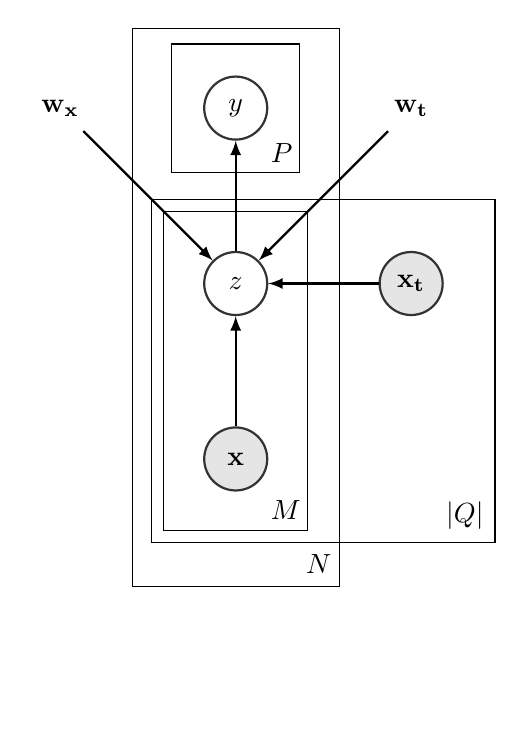
\begin{tikzpicture}
\tikzstyle{main}=[circle, minimum size = 8mm, thick, draw =black!80, node distance = 14mm]
\tikzstyle{mainnob}=[circle, minimum size = 8mm, thick, draw =white!100, node distance = 14mm]
\tikzstyle{connect}=[-latex, thick]
\tikzstyle{box}=[rectangle, draw=black!100]
\node[main, fill = white!100] (y) [label=center:$y$] { };
\node[rectangle, inner sep=-1mm, fit=(y),label=below right:$P$] {};
\node[rectangle, inner sep=4mm, fit=(y),draw=black!100] {};
\node[main, fill = white!100] (z) [below=of y,label=center:$z$] { };
%\node[rectangle, inner sep=-1mm, fit=(z),label=below right:$P$] {};
%\node[rectangle, inner sep=4mm, fit=(z),draw=black!100] {};
\node[main, fill = black!10] (x) [below=of z,label=center:$\mathbf{x}$] { }; 
\node[main, fill = black!10] (t) [right=of z,label=center:$\mathbf{x_t}$] { };
\node[mainnob, fill = white!100] (wt) [right=of y,label=center:$\mathbf{w_t}$] { };
\node[mainnob, fill = white!100] (wx) [left=of y,label=center:$\mathbf{w_x}$] { };
\node[rectangle, inner sep=-1mm, fit=(z)(x)(t),label=below right:$|Q|$, yshift=-1mm] {};
\node[rectangle, inner sep=6.5mm, fit=(z)(x)(t),draw=black!100] {};

\node[rectangle, inner sep=-1mm, fit=(z)(x),label=below right:$M$,yshift=-12mm] {};
\node[rectangle, inner sep=5.0mm, fit=(z)(x),draw=black!100] {};

\node[rectangle, inner sep=-1mm, fit=(x)(z)(y),label=below right:$N$,yshift=-30mm,xshift=4.5mm] {};
\node[rectangle, inner sep=9mm, fit=(x)(z)(y),draw=black!100, yshift=-3mm] {};

\path (wx) edge [connect] (z)
(x) edge [connect] (z)
(z) edge [connect] (y)
(wt) edge [connect] (z)
(t) edge [connect] (z);
\end{tikzpicture}
\caption{QnA-based relation extraction model plate diagram.
$N$ - number of different entity pairs, $M$ - number of mentions of an entity pair, $|Q|$ - number of questions where an entity pair is mentioned, $\mathbf{x}$ and $\mathbf{x_t}$ - mention-based and question-based features, $\mathbf{w}$ and $\mathbf{w_t}$ - corresponding feature weights, latent variables $z$ - relation expressed in an entity pair mention, latent variables $y$ - relations between entity pair}
\label{figure:qna_relextract:graphmodel}
\end{figure}

The proposed models for relation extraction from QnA data incorporates the topic of the question and can be represented as a graphical model (Figure \ref{figure:qna_relextract:graphmodel}).
Each mention of a pair of entities is represented with a set of mention-based features $x$ and question-based features $x_t$.
A multinomial latent variable $z$ represents a relation (or none) expressed in the mention and depends on the features and a set of weights $w_x$ for mention-based and $w_t$ for question-based features:
$$\hat{z}=\argmax{z \in P \cup \emptyset} p(z|x, x_t, w_x, w_t)$$.
To estimate this variable we use L2-regularized multinomial logistic regression model, trained using the distant supervision approach for relation extraction \cite{MintzBSJ09}, in which mentions of entity pairs related in Freebase are treated as positive instances for the corresponding predicates, and negative examples are sampled from mentions of entity pairs which are not related by any of the predicates of interest.
Finally, to predict a set of possible relations $\mathbf{y}$ between the pair of entities we take logical OR of individual mention variables $\mathbf{z}$, \ie $y_p = \lor_{i=1}^M [z_i = p, p \in P]$, where M is the number of mentions of this pair of entities.

\subsubsection{Sentence-based baseline model}
\label{section:factoid:approaches:cqarelextract:baseline}

Existing sentence-based relation extraction models can be applied to individual sentences of a QnA pair and will work well for complete statements, \eg ``Who did Brad Pitt marry? Brad Pitt and Angelina Jolie married at secret ceremony ...''.
In sentence-based scenario, when the set of question-based features is empty, the above model corresponds to the Mintz++ baseline described in \cite{Surdeanu:2012:MML:2390948.2391003}, which was shown to be superior to the original model of \cite{MintzBSJ09}, is easier to train than some other state of the art distant supervision models and produces comparable results.

\subsubsection{Sentence-based model with question features}
\label{section:factoid:approaches:cqarelextract:baselineqfeat}

\begin{table*}[tbh]
\centering
\begin{tabular}{|p{9cm}|p{7.8cm}|}
\hline
\multicolumn{2}{|c|}{Sentence-based model}\\
\hline
Dependency path between entities & \texttt{[PERSON]$\rightarrow$nsubjpass(born)tmod$\leftarrow$[DATE]}\\
Surface pattern & \texttt{[PERSON] be/VBD born/VBN [DATE]}\\
\hline
\hline
\multicolumn{2}{|c|}{Question features for sentence-based model}\\
\hline
Question template & \texttt{when [PERSON] born}\\
Dependecy path from a verb to the question word & \texttt{(when)$\rightarrow$advmod(born)}\\
Question word + dependency tree root & \texttt{when+born}\\
\hline
\hline
\multicolumn{2}{|c|}{QnA-based model}\\
\hline
Question template + answer entity type & \texttt{Q: when [PERSON] born A:[DATE]}\\
Dependency path from question word to entity & \texttt{Q:(when)$\rightarrow$advmod(born)nsubj$\leftarrow$[PERSON]}\\
and answer entity to the answer tree root & \texttt{A: (born)tmod$\leftarrow$[DATE]}\\
Question word, dependency root and answer pattern & \texttt{Q: when+born A:born [DATE]}\\
\hline
\end{tabular}
\caption{Examples of features used for relation extraction for ``\emph{When was Mariah Carey born? Mariah Carey was born 27 March 1970}''}
\label{table:qna_relextract:features}
\end{table*}

In many cases an answer statement is hard to interpret correctly without knowing the corresponding question.
To give the baseline model some knowledge about the question, we include question features (Table \ref{table:qna_relextract:features}), which are based on dependency tree and surface patterns of a question sentence. 
This information can help the model to account for the question topic and improve predictions in some ambiguous situations.

\subsubsection{QnA-based model}
\label{section:factoid:approaches:cqarelextract:qnamodel}

The QnA model for relation extraction is inspired by the observation, that often an answer sentence do not mention one of the entities at all, \eg, ``\textit{When was Isaac Newton born? December 25, 1642 Woolsthorpe, England}''.
To tackle this situation we make the following assumption about the discourse of a QnA pair: an entity mentioned in a question is related to entities in the corresponding answer and the context of both mentions can be used to infer the relation predicate.
Our QnA-based relation extraction model takes an entity from a question sentence and entity from the answer as a candidate relation mention, represents it with a set of features (Table \ref{table:qna_relextract:features}) and predicts a possible relation between them similar to sentence-based models.
The features are conjunctions of various dependency tree and surface patterns of question and answer sentences, designed to capture their topics and relation.

\subsubsection{Experiments}
\label{section:factoid:approaches:cqarelextract:experiments}

For experiments we used 2 publicly available CQA datasets: Yahoo! Answers WebScope dataset\footnote{http://webscope.sandbox.yahoo.com/catalog.php?datatype=l} and a crawl of WikiAnswers\footnote{http://wiki.answers.com/} collected by \cite{Fader:2014:OQA:2623330.2623677}.
The Yahoo! Answers dataset contains 4,483,032 questions (3,894,644 in English) with the corresponding answers collected on 10/25/2007.
The crawl of WikiAnswers has 30,370,994 question clusters, tagged by WikiAnswers users as paraphrases, and only 3,386,256 them have answers.
From these clusters we used all possible pairs of questions and corresponding answers (19,629,443 pairs in total).

\begin{table*}[ht]
\centering
\begin{tabular}{|p{12.5cm}||p{1.2cm}|p{1.2cm}|} \hline
& Y!A & WA\\
\hline
Number of QnA pairs & 3.8M & 19.6M \\
Average question length (in chars) & 56.67 & 47.03 \\
Average answer length (in chars) & 335.82 & 24.24 \\
% Number of resolved entities per QnA pair & 3.57 & 3.23 \\
Percent of QnA pairs with answers that do not have any verbs & 8.8\% & 18.9\% \\
Percent of QnA pairs with at least one pair of entities related in Freebase & 11.7\% & 27.5\% \\
Percent of relations between entity pairs in question sentences only & 1.6 \% & 3.1\% \\
Percent of relations between entity pairs in question and answer sentences only & 28.1\% & 46.4\% \\
Percent of relations between entity pairs in answer sentences only & 38.6\%& 12.0\%\\
\hline
\end{tabular}
\caption{Yahoo! Answers and WikiAnswers datasets statistics}
\label{table:qna_relextract:cqastats}
\end{table*}

For each QnA pair we applied tokenization, sentence detection, named entity tagger, parsing and coreference resolution from Stanford CoreNLP \cite{manning-EtAl:2014:P14-5}.
Our cascade entity linking approach is similar to \cite{chang2011stanford} and considered all noun phrase and named entity mentions as candidates.
First, all named entity mentions are looked up in Freebase names and aliases dictionary.
The next two stages attempt to match mention text with dictionary of English Wikipedia concepts \cite{spitkovsky2012cross} and its normalized version.
Finally for named entity mentions we try spelling correction using Freebase entity names dictionary.
We didn't disambiguate entities and instead took top-5 ids for each coreference cluster (using the $p(entity|phrase)$ score from the dictionary or number of existing Freebase triples).
All pairs of entities (or entity and date) in a QnA pair that are directly related\footnote{We also consider some paths that come through a mediator node, \eg  /people/person/spouse\_s./people/marriage/spouse} in Freebase were annotated with the corresponding relations.

Table \ref{table:qna_relextract:cqastats} gives some statistics on the datasets used in this work.
The analysis of answers that do not have any verbs show that $\sim$8.8\% of all QnA pairs do not state the predicate in the answer text.
The percentage is higher for WikiAnswers, which has shorter answers on average.
Unfortunately, for many QnA pairs we were unable to find relations between the mentioned entities (for many of them no or few entities were resolved to Freebase).
Among those QnA pairs, where some relation was annotated, we looked at the location of related entities.
In Yahoo! Answers dataset 38.6\% (12.0\% for WikiAnswers) of related entities are mentioned in answer sentences and can potentially be extracted by sentence-based model, and 28.1\% (46.4\% for WikiAnswers) between entities mentioned in question and answer sentences, which are not available to the baseline model and our goal is to extract some of them.

For our experiments we use a subset of 29 Freebase predicates that have enough unique instances annotated in our corpus, \eg date of birth, profession, nationality, education institution, date of death, disease symptoms and treatments, book author, artist album, \etc
We train and test the models on each dataset separately.
Each corpus is randomly split for training (75\%) and testing (25\%).
Knowledge base facts are also split into training and testing sets (50\% each).
QnA and sentence-based models predict labels for each entity pair mention, and we aggregate mention predictions by taking the maximum score for each predicate.
We do the same aggregation to produce a combination of QnA- and sentence-based models, \ie, all extractions produced by the models are combined and if there are multiple extractions of the same fact we take the maximum score as the final confidence.
The precision and recall of extractions are evaluated on a test set of Freebase triples, \ie an extracted triple is considered correct if it belongs to the test set of Freebase triples, which are not used for training (triples used for training are simply ignored).
Note, that this only provides a lower bound on the model performance as some of the predicted facts can be correct and simply missing in Freebase.

Figure \ref{figure:qna_relextract:pr_curve} shows Precision-Recall curves for QnA-based and sentence-based baseline models and some numeric results are given in Table \ref{table:qna_relextract:results}.
As 100\% recall we took all pairs of entities that can be extracted by either model.
It is important to note, that since some entity pairs occur exclusively inside the answer sentences and some in pairs of question and answer sentences, none of the individual models is capable of achieving 100\% recall, and maximum possible recalls for QnA- and sentence-based models are different.

\begin{figure}[h!]
\centering
\vspace{-2mm}
\begin{subfigure}[h]{0.45\textwidth}
	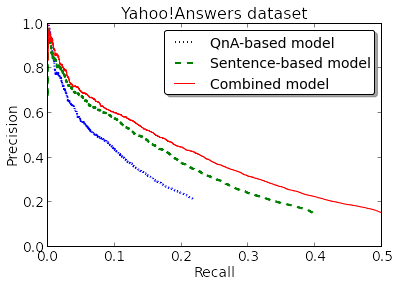
\includegraphics[width=0.99\textwidth]{img/cqarelextract_qa_vs_sent_ya}
	\vspace{-1mm}
    \label{figure:pr:ya}
\end{subfigure}
\begin{subfigure}[h]{0.45\textwidth}
	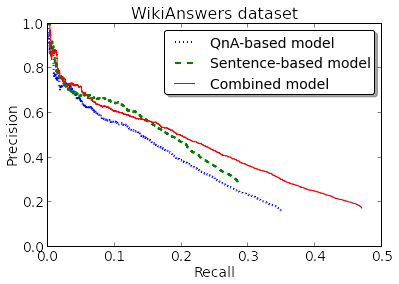
\includegraphics[width=0.99\textwidth]{img/cqarelextract_qa_vs_sent_wa}
	\vspace{-1mm}
    \label{figure:pr:wa}
\end{subfigure}
\begin{subfigure}[h]{0.45\textwidth}
	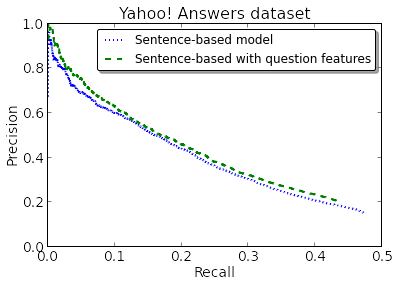
\includegraphics[width=0.99\textwidth]{img/cqarelextract_noqf_vs_qf}
	\vspace{-1mm}
	\label{figure:pr:noqf_vs_qf}
\end{subfigure}
\vspace{-1mm}
\caption{Precision-Recall curves for QnA-based vs sentence-based models and sentence-based model with and without question features}
\label{figure:qna_relextract:pr_curve}
\end{figure}

\begin{table*}[tbh]
\centering
\begin{tabular}{|p{6.6cm}||p{0.9cm}|p{1.4cm}|p{1.6cm}||p{0.9cm}|p{1.4cm}|p{1.6cm}|}
\hline
& \multicolumn{3}{|c||}{Yahoo! Answers} & \multicolumn{3}{|c|}{WikiAnswers}\\
\cline{2-7}
& QnA & Sentence & Combined & QnA & Sentence & Combined\\
\hline
F-1 score & 0.219 & 0.276 & 0.310 & 0.277 & 0.297 & 0.332\\
Number of correct extractions & 3229 & 5900 & 7428 & 2804 & 2288 & 3779 \\
Correct triples not extracted by other model & 20.5\% & 56.5\% & - & 39.4\% & 25.8\% & - \\
\hline
\end{tabular}
\caption{Extraction results for QnA- and sentence-based models on both datasets}
\label{table:qna_relextract:results}
\end{table*}

Results demonstrate that from 20.5\% to 39.4\% of correct triples extracted by the QnA-based model are not extracted by the baseline model, and the combination of both models is able to achieve higher precision and recall.
Unfortunately, comparison of sentence-based model with and without question-based features (Figure \ref{figure:qna_relextract:pr_curve}) didn't show a significant difference.

\subsubsection{Analysis}

To get an idea of typical problems of QnA-based model we sampled and manually judged extracted high confidence examples that are not present in Freebase (and thus are considered incorrect for precision-recall analysis).

The major reason (40\%) of false positive extractions is errors in entity linking.
For example: ``\emph{Who is Tim O'Brien? He was born in Austin on October 1, 1946}''.
The model was able to correctly extract [Tim O'Brien, date\_of\_birth, October 1, 1946], however Tim O'Brien was linked to a wrong person.
In a number of cases (16\%) our discourse model turns out to be too simple and fails for answers, that mention numerous additional information, \eg ``\emph{How old is Madonna really? ...Cher was born on 20 May 1946 which makes her older that Madonna...}''.
A possible solution would be to either restrict QnA-based model to cases when no additional information is present or design a better discourse model with deeper analysis of the answer sentence and its predicates and arguments.
Some mistakes are due to distant supervision errors, for example for the music.composition.composer predicate our model extracts singers as well as composers (which are in many cases the same).

Of course, there are a number of cases, when our extractions are indeed correct, but are either missing (33\%) or contradicting with Freebase (8\%).
An example of an extracted fact, that is missing in Freebase is ``\emph{Who is Wole Soyinka? He studied at the University College, Ibadan(1952-1954) and the University of Leeds (1954-1957)}'', and [Wole Soyinka, institution, University of Leeds] is currently not present in Freebase.
Contradictions with Freebase occur because of different precision levels (``pianist'' vs ``jazz pianist'', city vs county, \etc), different calendars used for dates or ``incorrect'' information provided by the user.
An example, when existing and extracted relation instance are different in precision is:``\emph{Who is Edward Van Vleck? Edward Van Vleck was a mathematician born in Middletown, Connecticut}'' we extract [Edward Van Vleck, place\_of\_birth, Middletown], however the Freebase currently has USA as his place of birth.

The problem of ``incorrect'' information provided in the answer is very interesting and worth special attention.
It has been studied in CQA research, \eg \cite{shah2010evaluating}, and an example of such QnA pair is: ``\emph{Who is Chandrababu Naidu? Nara Chandra Babu Naidu (born April 20, 1951)}''.
Other authoritative resources on the Web give April 20, 1950 as Chandrababu Naidu's date of birth.
This raises a question of trust to the provided answer and expertise of the answerer.
Many questions on CQA websites belong to the medical domain, \eg people asking advices on different health related topics.
How much we can trust the answers provided to extract them into the knowledge base?
We leave this question to the future work.

Finally, we have seen that only a small fraction of available QnA pairs were annotated with existing Freebase relations, which shows a possible limitation of Freebase schema.
A promising direction for future work is automatic extraction of new predicates, which users are interested in and which can be useful to answer more future questions.

\subsubsection{Summary}
\label{section:factoid:approaches:cqarelextract:summary}

In this section we described a model for relation extraction from QnA data, which is capable of predicting relations between entities mentioned in question and answer sentences.
We conducted experiments on 2 publicly available CQA datasets and showed that our model can extract triples not available to existing sentence-based techniques and can be effectively combined with them for better coverage of a knowledge base population system.

% =-=-=-=-=-=-=-=-=-=-Cqa Relation Extraction: End-=-=-=-=-=-=-=-=-=-=-=-=-=-=-

% =-=-=-=-=-=-=-=-=-=-=-=-=-=-Text2KB: Begin=-=-=-=-=-=-=-=-=-=-=-=-=-=-=-=-=-

\subsection{Text2KB: Knowledge Base Question Answering using External Text Data}
\label{section:factoid:approaches:text2kb}

Converting unstructured information into structured form by extracting knowledge from text suffers from certain quality losses.
Existing relation extraction tools aren't perfect, in particular due to recall losses a lot of information is left behind.
Moreover, extractions contain certain level of incorrect information due to precision losses.
These errors cap the upper bound on the question answering system performance.
In this section, I describe a novel factoid question answering system, that utilizes available textual resources to improve different stages of knowledge base question answering (KBQA).

KBQA systems must address three challenges, namely question entity identification (to anchor the query process); candidate answer generation; and candidate ranking.
We will show that these challenges can be alleviated by the appropriate use of external textual data.
Entity identification seeds the answer search process, and therefore the performance of the whole system greatly depends on this stage \cite{yao-scratch-qa-naacl2015}.
Question text is often quite short, may contain typos and other problems, that complicate entity linking.
Existing approaches are usually based on dictionaries that contain entity names, aliases and some other phrases, used to refer to the entities \cite{SPITKOVSKY12.266}.
These dictionaries are noisy and incomplete, \eg to answer the question \textit{``what year did tut became king?''} a system needs to detect a mention \textit{``tut''}, which refers to the entity \texttt{Tutankhamun}.
If a dictionary doesn't contain a mapping \textit{``tut''} $\rightarrow$ \texttt{Tutankhamun}, as happens for one of the state of the art systems, it will not be able to answer the question correctly.
Such less popular name variations are often used along with full names inside text documents, for example, to avoid repetitions.
Therefore, we propose to look into web search results to find variations of question entity names, which can be easier to link to a KB (Figure \ref{figure:text2kb:web_search_entitylink}).
This idea has been shown effective in entity linking for web search queries\footnote{http://web-ngram.research.microsoft.com/ERD2014/} \cite{SMAPH_ERD:2014}.

\begin{figure}[!ht]
\centering
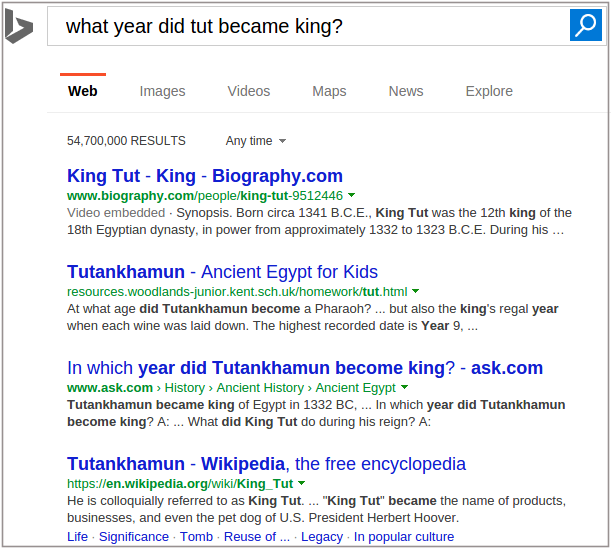
\includegraphics[width=0.5\textwidth]{img/web_search_entitylink}
\caption{Search results for the question \textit{``what year did tut became king?''}, which mention both the full name of the king and the correct answer to the question}
\label{figure:text2kb:web_search_entitylink}
\end{figure}

After question entities have been identified, answer candidates need to be generated and ranked to select the best answer.
A candidate query includes one or multiple triple patterns with predicates, corresponding to words and phrases in the question.
Existing knowledge base question answering approaches \cite{bastmore:cikm:2015:aquu,BerantCFL13:sempre,BerantL14:parasempre,berant2015imitation,BordesCW14:emnlp,yao2014freebase} rely on a lexicon, learned from manually labeled training data, and supported by additional resources, such as question paraphrases \cite{BerantL14:parasempre} and weakly labeled sentences from a large text collection \cite{YaoD14}.
Such training data tends to be small compared to the number of different predicates in a KB, and therefore the coverage of these lexicons is limited.
By our estimate, in a popular WebQuestions KBQA dataset~\cite{BerantCFL13:sempre}, the answers to $\sim$5.5\% of test questions (112 out of 2032) involve a predicate that does not appear as a ground truth in the training set.
For example, an RDF triple \texttt{[Bigos, food.dish.type\_of\_dish1, Stew]} answers the question \textit{``what are bigos?''}, but no other examples in the training set involve this predicate.
In addition, a lexicon needs to cover all different ways a predicate can be asked about.
For example, questions \textit{``who did jon gosselin cheat with?''} and \textit{``who is the woman that john edwards had an affair with?''} are answered by the same KB predicate, but use different language.
Therefore, presence of the first question in a training set may not help to answer the second question.
On the other hand, traditional Text-QA systems benefit from the redundancy of the information on the Web, where the same facts are stated multiple times in many different ways \cite{lin2007exploration}.
This increases the chances of a good lexical match between a question and answer statements, which makes even some relatively simple counting-based techniques quite effective \cite{brill2002analysis}.
We propose to adapt these ideas from text-based question answering for KBQA.

The general architecture and an example use case of Text2KB is presented on Figure \ref{figure:text2kb:model}.
Text2Kb is based on the information extraction approach to knowledge base question answering \cite{YaoD14}, in particular it extends the Aqqu system of H.Bast et al.~\cite{bastmore:cikm:2015:aquu}, which is one of the best performing open source KBQA system on the WebQuestions dataset.
The left part of the Figure \ref{figure:text2kb:model} describes a typical architecture of IE-based KBQA systems, and the right part introduces additional external text data sources, namely Web search results, community question answering (CQA) data, and a collection of documents with detected KB entity mentions.
First, we describe the main stages of the information extraction approach to knowledge base question answering using Aqqu, our baseline system, as an example.

\begin{figure*}[!ht]
\centering
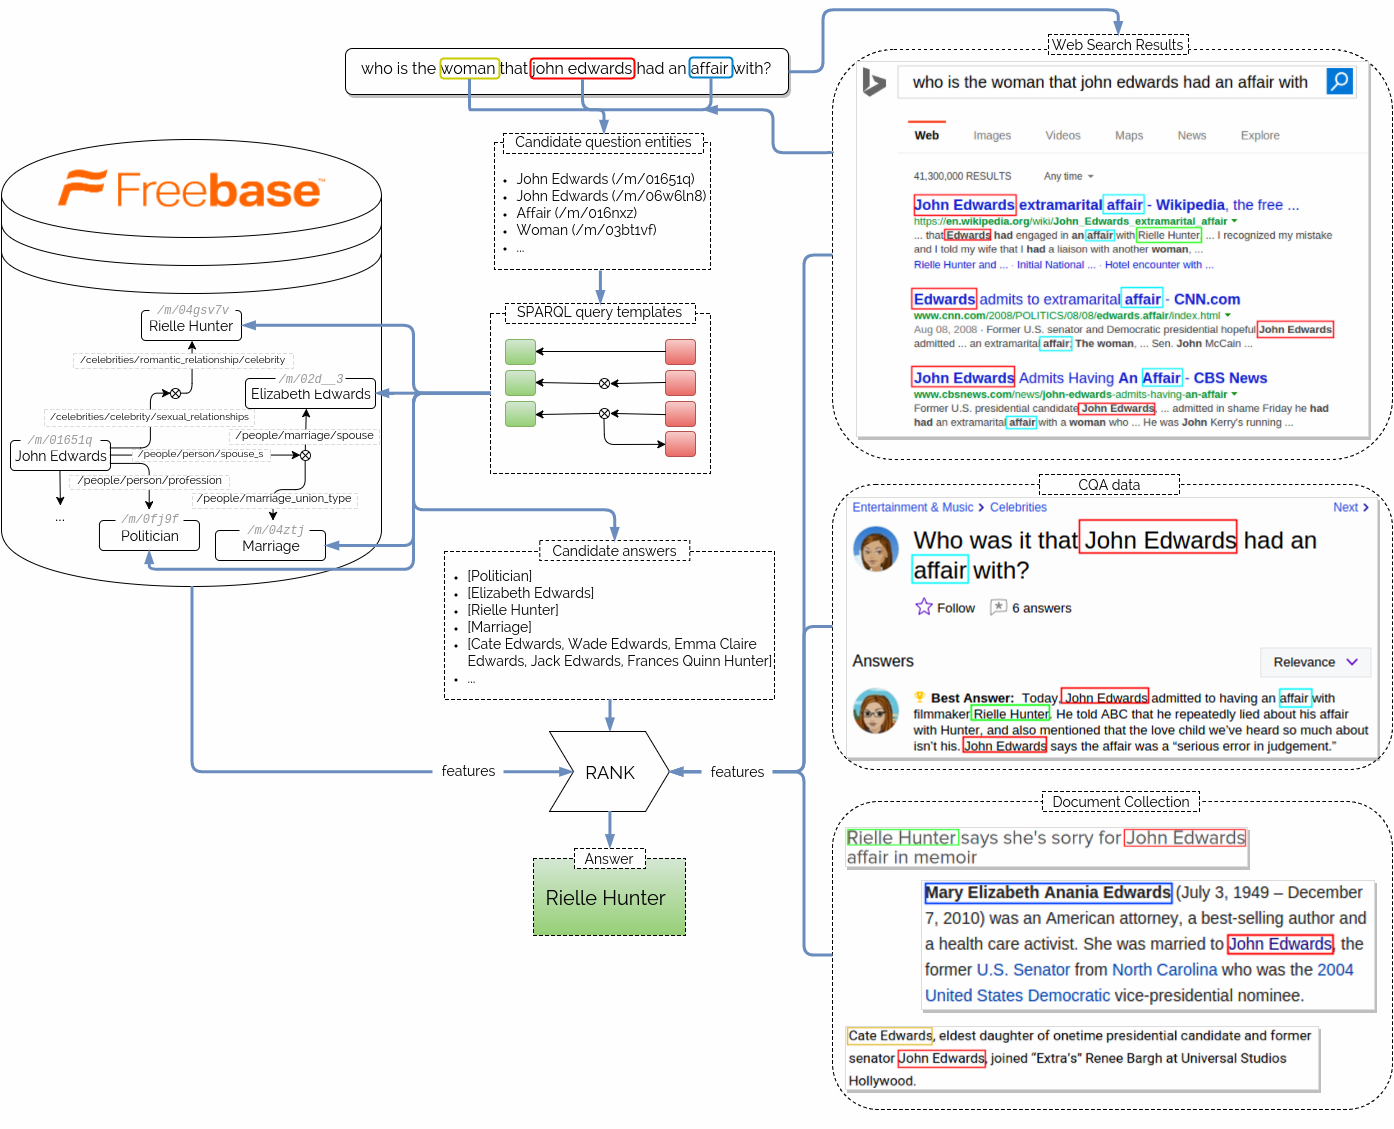
\includegraphics[width=\textwidth]{img/text2kb_model}
\caption{The architecture of our Text2KB Question Answering system}
\label{figure:text2kb:model}
\end{figure*}

\subsubsection{Information Extraction Approach to KBQA}
\label{section:factoid:approaches:text2kb:baseline}

The first stage of the knowledge base question answering process is identification of question topic entities, which are used as sources for the answer search process.
For concreteness, consider a question from the WebQuestions dataset \textit{``who is the woman that john edwards had an affair with?''}.
Here, the entity \texttt{John Edwards} with Freebase id \texttt{/m/01651q} is the main question entity.
However, Freebase contains millions of entities and it can be difficult to identify the topical ones (\eg entities \texttt{Woman} and \texttt{Affair} are also present in Freebase), or to disambiguate and choose between \texttt{John Edwards} a politician (\texttt{/m/01641q}), an American racing driver (\texttt{/m/06zs089}) and other people with the same name.
Aqqu considers all spans of question words under certain conditions on part of speech tags and uses an entity names lexicon \cite{SPITKOVSKY12.266} to map phrases to potential entities.
Most reported systems, including Aqqu, do not disambiguate entities at this stage, but rather keep a set of candidates along with some information about their popularities (\eg number of mentions in the collection), and mention scores $p(entity| mention\ text)$.

At the next stage, SPARQL query candidates are generated by exploring the neighborhood of the question topic entities using a predefined set of query templates.
Each query template has question entities, predicates and answer placeholders.
The majority of the answers in the WebQuestions dataset can be covered by just 3 templates (q\_entity - question entity, a\_entity - answer entity, cvt\_node - Freebase mediator node, which represent tuples with more than 2 arguments):
\\

\begin{lstlisting}[frame=single,basicstyle=\small]
SELECT DISTINCT ?a_entity {
   <q_entity> <predicate> ?a_entity .
}
\end{lstlisting}

\begin{lstlisting}[frame=single,basicstyle=\small]
SELECT DISTINCT ?a_entity {
   <q_entity> <predicate_1> ?cvt_node .
   ?cvt_node <predicate_2> ?a_entity .
}
\end{lstlisting}

\begin{lstlisting}[frame=single,basicstyle=\small]
SELECT DISTINCT ?a_entity {
   <q_entity_1> <predicate_1> ?cvt_node .
   ?cvt_node <predicate_2> <q_entity_2> .
   ?cvt_node <predicate_3> ?a_entity .
}
\end{lstlisting}

The first template retrieves a set of entities that are directly connected to the given question entity via a certain predicate.
The second template accounts for the presence of a mediator node, that groups together arguments of a multi-argument relation.
And the last template looks for cases, when a question also mentions another argument of a multi-argument relation, \eg \texttt{Captain Kirk} and \texttt{Star Trek} for the question \textit{``who played captain kirk in star trek movie?''}.

Each query candidate is represented with a set of features, that includes the scores for linked question entities, various scores for matching between question term n-grams and query predicates, the size of the results list, \etc
The final stage of the question answering process is filtering and ranking.
The Aqqu system employs a pairwise learning-to-rank model, trained on part of the dataset.
For each pair of candidate answers Aqqu creates an instance, which contains 3 groups of features: features of the first, the second candidate in the pair and the differences between the corresponding features of the candidates. Specifically, a Random Forest model is used in the provided Aqqu implementation. 
A pair where the first candidate is better than the second belongs to class +1, and -1 otherwise.
To reduce the number of pairs for the final ranking, Aqqu includes a simplified linear filtering model, which is trained to detect incorrect answers with high precision. 

In Text2KB we also introduced a couple of extensions to the original Aqqu system, which doesn't involve external text data.
We noticed that since Aqqu does not use information about the answer entity Freebase types, in many cases it returns an answer that is incompatible with the question: \eg state instead of county \etc
Therefore, we trained a model to return a score that measures compatibility between the question and answer entities, based on the entity notable types and question uni- and bi-grams as features, similar to Aqqu's relations score model.
A second extension introduced a new date range query template, which helps solve cases like \textit{``what team did david beckham play for in 2011?''}, where we need to look at the ranges of dates to determine whether an answer candidate satisfies the question.

\begin{lstlisting}[frame=single,basicstyle=\small]
SELECT DISTINCT ?a_entity {
   <q_entity_1> <predicate_1> ?cvt_node .
   ?cvt_node <from_predicate> ?date_from .
   ?cvt_node <to_predicate> ?date_to .
   ?cvt_node <predicate_2> ?a_entity .
   FILTER ( <question_date> >= ?date_from AND
            <question_date> <= ?date_to )
}
\end{lstlisting}

\subsubsection{Text2KB model}
\label{section:factoid:approaches:text2kb:model}

Now, let's look into the improvements introduced in Text2KB by employing various textual resources.

\textbf{Web search results for KBQA}

Traditional Text-QA systems rely on search results to retrieve relevant documents, which are then used to extract answers to users' questions.
Relevant search results mention question entities multiple times and in various forms, which can be helpful for entity linking \cite{SMAPH_ERD:2014}.
Furthermore, retrieved document set often contains multiple statements of the answer, which can be a strong signal for candidate ranking \cite{lin2007exploration}.

To obtain related web search results, Text2KB issues the question as a query to a search engine\footnote{In our experiments we use the Bing Web Search API https://datamarket.azure.com/dataset/bing/search and local Wikipedia search using Lucene}, extracts top 10 result snippets and the corresponding documents.
Next, Text2KB uses Aqqu entity linking module to detect KB entity mentions in both snippets and documents.

Question text provides only a limited context for entity disambiguation and linking; additionally, the entity name can be misspelled or an uncommon variation used.
This complicates the task of entity identification, which is the foundation of KB question answering process.
Fortunately, web search results help with these problems, as they usually contain multiple mentions of the same entities and provide more context for disambiguation.
Text2KB uses the search result snippets to \textit{expand} the set of detected question entities.
More specifically, we count the frequencies of each entity mentioned in search snippets, and most popular ones with names similar to some of the question terms are added to the list of topical entities.
The goal of this similarity condition is to keep only entities that are likely mentioned in the question text, and filter out related, but different entities.
To estimate the similarity between a name and question tokens, we use Jaro-Winkler string distance.
An entity is added to the list of question entities if at least one of its tokens $e_t$ has high similarity with one of the question tokens $q_t$ excluding stopwords ($Stop$):
$$max_{e_t \in M \backslash Stop, q_t \in Q \backslash Stop} 1 - dist(e_t, q_t) \geq 0.8$$

The information stored in KBs can also be present in other formats, \eg text statements.
For example, on Figure \ref{figure:text2kb:web_search_entitylink} multiple search snippets mention the date when Tutankhamun became a king.
Text-QA systems use such passages to extract answer to users' questions.
However, text may not provide sufficient context information about the mentioned entities, and systems have to infer the useful details, \eg entity types, which can be problematic \cite{yih2014semantic}.
On the other hand, KBQA systems can utilize all the available KB knowledge about the entities in a candidate answer, and would benefit from additional text-based information to improve ranking.
More specifically, Text2KB proceeds as follows:

\begin{enumerate}
\item Precompute term and entity IDFs. We used Google n-grams corpus to approximate terms IDF by collection frequencies and available ClueWeb Freebase entity annotations\footnote{http://lemurproject.org/clueweb09/FACC1/} to compute entity IDF scores.
\item Each snippet $s_i$ and document $d_i$ are represented by two TF-IDF vectors of lowercased tokens ($t_{s_i}$ and $t_{d_i}$) and mentioned entities ($e_{s_i}$ and $e_{d_i}$).
\item In addition, vectors of all snippets and all documents are merged together to form combined token and entity vectors: $t_{\cup s_i}$, $t_{\cup d_i}$, $e_{\cup s_i}$ and $e_{\cup d_i}$.
\item Each answer candidate $a_j$ is also represented as TF-IDF vector of terms (from entity names), and entities: $t_{a_j}$ and $e_{a_j}$
\item Cosine similarities between answer and each of 10 snippet and document vectors are computed: $\cos(t_{s_i}, t_{a_j})$, $\cos(t_{d_i}, t_{a_j})$ and $\cos(e_{s_i}, e_{a_j})$, $\cos(e_{d_i}, e_{a_j})$.
We use the average score and the maximum score as features.
\item We also compute answer similarities with the combined snippet and document vectors: $\cos(t_{\cup s_i}, t_{a_j})$, $\cos(e_{\cup s_i}, e_{a_j})$, $\cos(t_{\cup d_i}, t_{a_j})$, $\cos(e_{\cup d_i}, e_{a_j})$.
\end{enumerate}

\textbf{CQA data for Matching Questions to Predicates}

Recall that a major challenge in KBQA is that natural language questions do not easily  map to entities and predicates in a KB.
An established approach for this task is supervised machine learning, which requires labeled examples of questions and the corresponding answers to learn this mapping, which can be expensive to construct.
Researchers have proposed to use weakly supervised methods to extend a lexicon with mappings learned from \textit{single sentence statements} mentioning entity pairs in a large corpus \cite{YaoD14}.
However, the language used in questions to query about a certain predicate may differ from the language used in statements.
In Section~\ref{section:factoid:approaches:cqarelextract} we demonstrated how distant supervision can be applied to question-answer pairs from CQA archives for a related task of information extraction for knowledge base completion.
In a similar way, we use weakly labeled collection of question-answer pairs to compute {\em associations} between question terms and predicates to \textit{extend} system's lexicon (Figure \ref{figure:text2kb:cqa_example}).
We emphasize that this data does not replace the mappings learned from single sentence statements, which are already used by our baseline system, but rather introduces the new ones learned from the CQA data.

\begin{figure}
\centering
\fbox{
 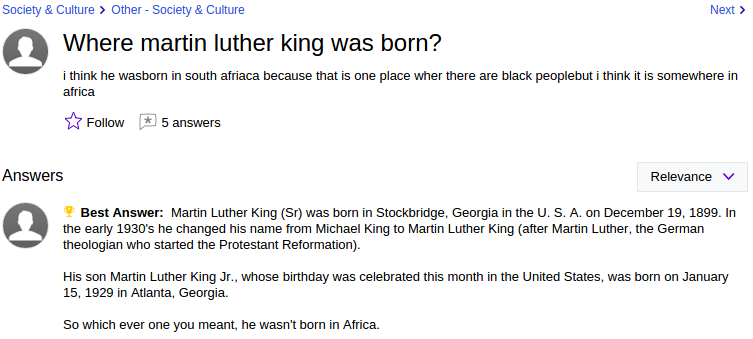
\includegraphics[width=0.5\textwidth]{img/cqa_example}
}
\caption{Example of a question and answer pair from Yahoo! Answers CQA website}
\label{figure:text2kb:cqa_example}
\end{figure}

For our experiments we use 4.4M questions from Yahoo! WebScope L6 dataset\footnote{https://webscope.sandbox.yahoo.com/}.
Question and answer texts were run through an entity linker, that detected mentions of Freebase entities.
Next, we use distant supervision assumption to label each question-answer pair with predicates between entities mentioned in the question and in the answer.
This labels are used to learn associations between question terms and predicates by computing pointwise mutual information scores (PMI) for each term-predicate pair.
Examples of scores for some terms are given in Table \ref{table:text2kb:cqa_npmi}.

\begin{table}
\centering
\begin{tabular}{| p{2cm} | p{8.5cm} | p{1cm} |}
\hline
Term & Predicate & PMI score\\
\hline
born & \texttt{people.person.date\_of\_birth} & 3.67\\
 & \texttt{people.person.date\_of\_death} & 2.73\\
 & \texttt{location.location.people\_born\_here} & 1.60\\
\hline
kill & \texttt{people.deceased\_person.cause\_of\_death} & 1.70\\
& \texttt{book.book.characters} & 1.55\\
\hline
currency & \texttt{location.country.currency\_formerly\_used} & 5.55 \\
& \texttt{location.country.currency\_used} & 3.54 \\
\hline
school & \texttt{education.school.school\_district} & 4.14 \\
& \texttt{people.education.institution} & 1.70\\
& \texttt{sports.school\_sports\_team.school} & 1.69 \\
\hline
illness & \texttt{medicine.symptom.symptom\_of} & 2.11\\
& \texttt{medicine.decease.causes} & 1.68\\
& \texttt{medicine.disease.treatments} & 1.59\\
\hline
win & \texttt{sports.sports\_team.championships} & 4.11\\
& \texttt{sports.sports\_league.championship} & 3.79\\
\hline
\end{tabular}
\caption{Examples of term-predicate pairs with high PMI scores, computed using distant supervision from a CQA collection}
\label{table:text2kb:cqa_npmi}
\end{table}

In Text2KB we evaluate candidate answer predicates by using the association (e.g., PMI) scores between predicates and the question terms (missing pairs are given a score of 0).
The minimum, average and maximum of these values are used as features to represent a candidate answer.
Such associations data can be sparse, we also use pretrained word2vec word embeddings\footnote{https://code.google.com/p/word2vec/}.
We compute predicate embeddings by taking a weighted average of term vectors from predicate's PMI table.
Each term vector is weighted by its PMI value (terms with negative score are skipped).
Then, we compute cosine similarities between predicate vector and each of the question term vectors and take their minimum, average, maximum as features.
Finally, we average embeddings of question terms and compute its cosine similarity with the predicate vector.

\textbf{Estimating Entity Associations}

A key step for ranking candidate answers is to estimate whether the question and answer entities are related in a way asked in the question.
Existing KBQA approaches usually focus on scoring the mappings between question phrases and KB concepts from a candidate SPARQL query.
However, textual data can provide another angle on the problem, as question and answer entities are likely to be mentioned together somewhere in text passages.
For example, in the bottom right corner of Figure \ref{figure:text2kb:model} we can see some passages that mention a pair of people, and the context of these mentions explains the nature of the relationships.
This data can be viewed as additional edges in a KB, which connect pairs of entities, and have associated language models, estimated from text phrases, that mention these entities.
Such edges do not have to coincide with the existing KB edges, and can connect arbitrary pairs of entities, that are mentioned together in text, therefore extending the KB.

We use the ClueWeb12 corpus with existing Freebase entity annotations and count different terms that occur in the context of a mention of a pair of different entities (we only consider mentions within 200 characters of each other).
To compute this unigram language model we use the terms separating the entities, as well as the terms within a small window (e.g., 100 characters) before and after the entity mentions.
A small sample of this data is presented in Table \ref{table:text2kb:clueweb_entitypairs_langmodel}.

\begin{table}
\centering
\begin{tabular}{| p{3.5cm} | p{3.5cm} | p{9cm} |}
\hline
Entity 1 & Entity 2 & Term counts\\
\hline
John Edwards & Rielle Hunter & campaign, affair, mistress, child, former ...\\
\hline
John Edwards & Cate Edwards & daughter, former, senator, courthouse, greensboro, eldest ...\\
\hline
John Edwards & Elizabeth Edwards & wife, hunter, campaign, affair, cancer, rielle, husband ...\\
\hline
John Edwards & Frances Quinn & daughter, john, rielle, father, child, former, paternity...\\
\hline
\end{tabular}
\caption{Example of entity pairs along with the most popular terms mentioned around the entities}
\label{table:text2kb:clueweb_entitypairs_langmodel}
\end{table}

We use this data to compute candidate ranking features as follows.
Consider question words $Q$ and an answer candidate, which contains a question entity $e_1$ and one or more answer entities $e_2$.
For each answer candidate, we compute a language model score:
$$p(Q|e_1, e_2) = \prod_{t\in Q} p(t | e_1, e_2)$$
and use the minimum, average and maximum over all answer entities as features.
To address the sparsity problem, we again use embeddings, 
\ie for each entity pair a weighted (by counts) average embedding vector of terms is computed and minimum, average and maximum cosine similarities between these vectors and question token embeddings are used as features.

\textbf{Internal text data to enrich entity representation}
In addition to external text data, many knowledge bases, including Freebase, contain text data as well, \eg Freebase includes a description paragraph from Wikipedia for many of its entities.
These text fragments provide a general description of entities, which may include information relevant to the question \cite{Sun:2015:ODQ:2736277.2741651}.
For completeness, we include them in our system as well.
Each entity description is represented by a vector of tokens, and a vector of mentioned entities.
We compute cosine similarities between token and entity vectors of the question and description of each of the answers, and use the minimum, average and maximum of the scores as features.

\subsubsection{Evaluation}
\label{section:factoid:approaches:text2kb:eval}

\begin{table*}[ht!]
\centering
\begin{tabular}{| p{5.2cm} | c | c | c | c | }
\hline
System & \centering{avg Recall} & \centering{avg Precision} & \centering{F1 of avg P and R} & avg F1 \\
\hline
OpenQA \cite{Fader:2014:OQA:2623330.2623677} & - & - & - & 0.35 \\
YodaQA \cite{baudivs2015yodaqa} & - & - & - & 0.343 \\
\hline
Jacana \cite{YaoD14} & 0.458 & 0.517 & 0.486 & 0.330\\
SemPre \cite{BerantCFL13:sempre} & 0.413 & 0.480 & 0.444 & 0.357\\
Subgraph Embeddings \cite{BordesCW14:emnlp} & - & - & 0.432 & 0.392\\
ParaSemPre \cite{BerantL14:parasempre} & 0.466 & 0.405 & 0.433 & 0.399\\
Kitt AI \cite{yao-scratch-qa-naacl2015} & 0.545 & 0.526 & 0.535 & 0.443\\
AgendaIL \cite{berant2015imitation} & 0.557 & 0.505 & 0.530 & 0.497\\
STAGG \cite{yih2014semantic} & 0.607 & 0.528 & 0.565 & 0.525\\
FMN \cite{jain2016question} & \textbf{0.649} & \textbf{0.552} & \textbf{0.597} & \textbf{0.557}\\
\hline
Aqqu (baseline) \cite{bastmore:cikm:2015:aquu} & 0.604 & 0.498 & 0.546 & 0.494\\
Text2KB (Wikipedia search) & \textbf{0.632}$^*$ \tiny{(+4.6\%)} & 0.498 & 0.557$^*$ \tiny{(+2.0\%)} & 0.514$^*$ \tiny{(+4.0\%)} \\
Text2KB (Web search) & \textbf{0.635}$^*$ \tiny{(+5.1\%)} & 0.506$^*$ \tiny{(+1.6\%)} & \textbf{0.563}$^*$ \tiny{(+3.1\%)} & \textbf{0.522}$^*$ \tiny{(+5.7\%)} \\
\hline
\end{tabular}
\caption{Performance of the Text2KB system on WebQuestions dataset compared to the existing approaches. The differences of scores marked * from the baseline Aqqu system are significant with p-value $<$ 0.01}
\label{table:text2kb:webquestions_results}
\end{table*}

This section reports the experimental setup, including the dataset and metrics, as well as the main methods compared for evaluating the performance of our Text2KB system. Additionally, we describe a series of ablation studies to analyze contribution of different system components.

textbf{Methods Compared}.
We compare our system, Text2KB, to state-of-the-art approaches, notably:
\begin{itemize}
\item{\textbf{Aqqu}}: the state-of-the-art baseline KBQA system~\cite{bastmore:cikm:2015:aquu}, described in Section 2.
\item{\textbf{Text2KB(Web search)}}: Our Text2KB system, using the Bing search engine API over the Web. 
\item{\textbf{Text2KB(Wikipedia search)}}: Our Text2KB system, using the standard Lucene search engine over the February 2016 snapshot of the English Wikipedia, in order to validate our system without the potential ``black-box'' effects of relying on a commercial Web search engine (Bing) and changing corpus (Web).
\item{\textbf{STAGG}}: The current\footnote{At the moment of our paper publication, FMN system of \cite{jain2016question} later improved the state-of-the-art} highest performing KBQA system~\cite{yih:ACL:2015:STAGG} as measured on the WebQuestions dataset.
\end{itemize}
Additionally, other previously published results on WebQuestions are included to provide context for the improvements introduced by our Text2KB system.

\textbf{Datasets}.
We followed the standard evaluation procedure for the WebQuestions dataset, and used the original 70-30\% train-test split (3,778 training and 2,032 test instances). Within the training split, 10\% was set aside for validation to tune the model parameters and only the best-performing set of parameters selected on the validation data was used to report the results on the official test split.

\textbf{Evaluation Metrics}. 
Recent papers using the WebQuestions dataset have primarily used the average F1-score as the main evaluation metric, defined as:
$avg\ F1 = \frac{1}{|Q|} \sum_{q \in Q} f1(a^*_q, a_q)$
$$f1(a^*_q, a_q) = 2\frac{precision(a^*_q,a_q) recall(a^*_q,a_q)}{precision(a^*_q,a_q) + recall(a^*_q,a_q)}$$
$precision(a^*_q, a_q)=\frac{|a^*_q \cap a_q|}{|a_q|}$ and $recall(a^*_q, a_q) = \frac{|a^*_q \cap a_q|}{|a^*_q|}$, $a^*_q$ and $a_q$ are correct and given answers to the question q, which can be lists of entities.
Additionally, we report average precision and recall, to gain better understanding of the tradeoffs achieved by different methods.

\textbf{Main Results}.
The results of existing approaches and our Text2KB system are presented in Table \ref{table:text2kb:webquestions_results}.
We should note, that text-based QA systems typically return a ranked list of answers, whereas many answers on WebQuestions dataset are lists, which complicates the comparison between KBQA and text-based systems.
The result reported for YodaQA system is F1 score at position 1.

As we can see, Text2KB significantly improves over the baseline system and reaches the current best published result - STAGG~\cite{yih:ACL:2015:STAGG}. 
We believe that this system will also benefit from the ideas of our work.

\textbf{Datasource and Features Contribution}.
To analyze the contribution of the features and data sources we introduced, we report results from a series of ablation studies. For convenience, we introduce the following short-hand notations for different components of our system:

\begin{itemize}
\item \texttt{T} - notable type score model as a ranking feature
\item \texttt{DF} - date range filter-based query template
% \item TF - using notable type based filter
\item \texttt{WebEnt} - using web search result snippets for question entity identification
\item \texttt{WikiEnt} - using wikipedia search result snippets for question entity identification
\item \texttt{Web} - using web search results for feature generation
\item \texttt{Wiki} - using wikipedia search results for feature generation
\item \texttt{CQA} - using CQA-based \texttt{[question term, KB predicate]} PMI scores for feature generation
\item \texttt{CW} - features, computed from entity pairs language model, estimated on ClueWeb
\end{itemize}

In our results table we will use the notation \texttt{+$<$comp$>$} for a system with a certain component added, and \texttt{-$<$comp$>$} when it is removed.
For example, the baseline system will be denoted as ``\texttt{Aqqu}''.
The same system with additional date range filter query templates and notable types score model is denoted as ``\texttt{Aqqu +DF+T}'', which represents the same system as ``\texttt{Text2KB -WebEnt-Web-CQA-CL}'' (we will call it Text2KB (base)).
Our full system ``\texttt{Text2KB}'' can be also denoted as ``\texttt{Aqqu +DF+T+WebEnt+Web+CQA+CL}''.

First, we analyze the improvements introduced by different components of our system (Table \ref{table:text2kb:ablation:entities_vs_features}).
As we can see, additional date range filters and notable types model (\texttt{Aqqu+DF+T}) are responsible for an increased recall and a drop in precision compared to the baseline model.
Features generated from Wikipedia search results, CQA data and ClueWeb entity pair language models (\texttt{+Wiki+CQA+CL}) improve average F1 by 0.007 (+1.4\%) compared to the base model, adding entity linking using Wikipedia search results improves results even more (+3\%).

Web search results (\texttt{+Web+CQA+CL}) turned out to be more helpful than Wikipedia results (\texttt{+Wiki+CQA+CL}), which is natural since Wikipedia is a subset of the web.
This was one of the reasons we didn't combine Wikipedia and Web search together.
Finally, entity linking and all text-based features combined achieves an even higher score, proving that their contributions are independent.

We now anylize the contribution of the different data sources.
We will remove a group of web search, CQA or Clueweb-based features and see how the performance of the whole system changes (Table \ref{table:text2kb:ablation:features}).
As we can see, all data sources have an impact on the system performance, and web search results based features provide the most useful signal for answer ranking.

Figure \ref{figure:text2kb:feature_importances} plots a subset of features ranked by their Gini index-based importance scores.
The figure supports the observation that web search results features are the most useful, however, other text data sources also contribute to the improvement.

\begin{table}[h]
\centering
\begin{tabular}{| p{6cm} | c | c | c | }
\hline
System & R & P & F1 \\
\hline
\texttt{Aqqu} & 0.604 & 0.498 & 0.494\\
\texttt{Text2KB (base) = Aqqu+DF+T} & 0.617 & 0.481 & 0.499 \\
\hline
\texttt{+Wiki+CQA+CL} & 0.623 & 0.487 & 0.506 \\
\texttt{+WikiEnt +Wiki+CQA+CL} & 0.632 & 0.498 & 0.514 \\
\hline
\texttt{+WebEnt} & 0.627 & 0.492 & 0.508 \\
\texttt{+Web+CQA+CL} & 0.634 & 0.497 & 0.514 \\
\texttt{+WebEnt +Web+CQA+CL} & 0.635 & 0.506 & 0.522 \\
\hline
\end{tabular}
\caption{Average Recall (R), Precision (P), and F1 of Aqqu and Text2KB system with and without different components. +A means that a component A is added to the Text2KB (base) system.}
\label{table:text2kb:ablation:entities_vs_features}
\end{table}

\begin{table}[h]
\centering
\begin{tabular}{| p{6cm} | c | c | c | }
\hline
System & R & P &  F1 \\
\hline
Text2KB (Web search) & 0.635 & 0.506 & 0.522 \\
\hline
% THIS PART ANSWERS HOW GOOD ARE EACH OF THE PROPOSED DATASETS
% extent_cqa_clueweb_dates_typemodel_rf100.log : -web
\texttt{Text2KB -Web} & 0.633 & 0.496 & 0.513 \\
% extent_web_clueweb_dates_typemodel_rf100.log : -cqa
\texttt{Text2KB -CQA} & 0.642 & 0.499 & 0.519 \\
% extent_web_cqa_dates_typemodel_rf100.log : -clueweb
\texttt{Text2KB -CL} & 0.644 & 0.505 & 0.523 \\
\hline
% extent_web_dates_typemodel_rf100.log : -clueweb-cqa
\texttt{Text2KB -CQA-CL} & 0.642 & 0.503 & 0.522 \\
% extent_clue_dates_typemodel_rf100.log : -web-cqa
\texttt{Text2KB -Web-CQA} & 0.631 & 0.498 & 0.514 \\
% extent_cqa_dates_typemodel_rf100.log : -web-clueweb
\texttt{Text2KB -Web-CL} & 0.622 & 0.493 & 0.508 \\
%\hline
% extent_web_cqa_clueweb_dates_types_typemodel_rf100.log : everything, including type filters
%\texttt{Text2KB} & 0.6354 & 0.5059 & 0.5223 \\
\hline
\end{tabular}
\caption{Average Recall (R), Precision (P), and F1 of Text2KB with and without features based on web search results, CQA data and ClueWeb collection.}
\label{table:text2kb:ablation:features}
\end{table}

\begin{figure*}
\centering
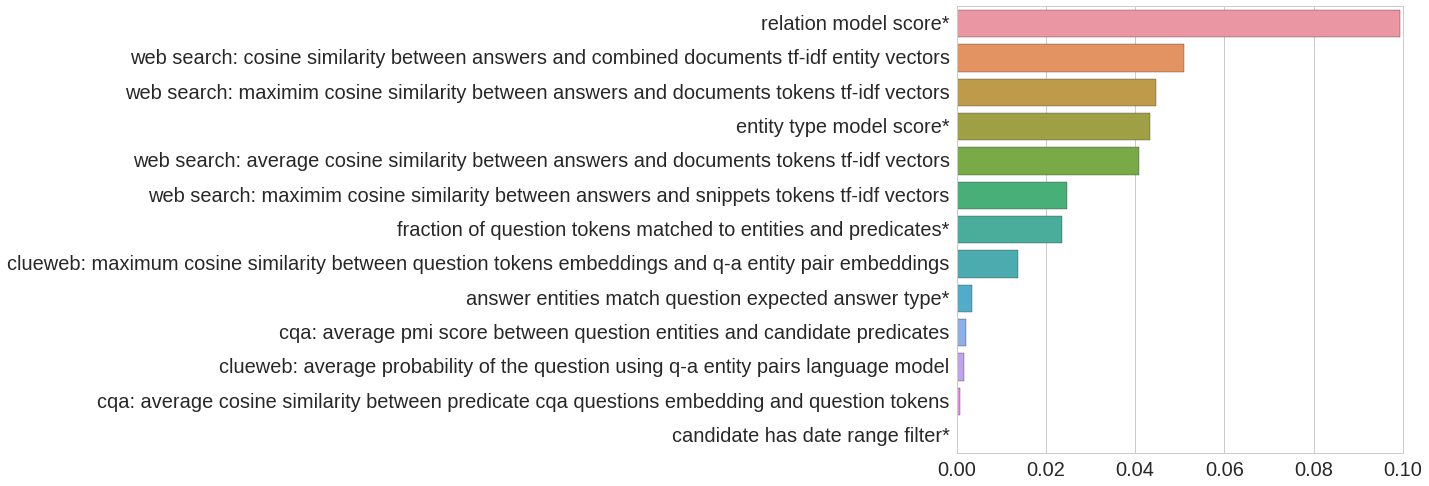
\includegraphics[width=\textwidth]{img/feature_importances}
\caption{A plot of Gini importances of different features of our answer ranking random forest model (features marked * are not text-based and are provided for comparison)}
\label{figure:text2kb:feature_importances}
\end{figure*}

In summary, Text2KB significantly outperforms the baseline system, and each of the introduced components contributes to this improvement.
Web search results data turned out to be the most useful resource, and it significantly improves the quality by helping with question entity identification and candidate ranking.
Next, we analyze the system performance in more detail, and investigate factors for future extension.

\subsubsection{Analysis}
\label{section:factoid:approaches:text2kb:analysis}

We now investigate how our system would compare to other systems on the same benchmark; then, we investigate in depth the different error modes, which helps identify the areas of most substantial future improvements.

We took an existing KBQA systems and demonstrated that by combining evidence from knowledge base and external text resources we can boost the performance.
A reasonable question is whether the same approach will be helpful to other systems, \eg the currently best system -- STAGG~\cite{yih:ACL:2015:STAGG}.
STAGG differs from our baseline system Aqqu in the components: entity linking algorithm, a set of query templates and ranking methods.
Therefore, our approach is complementary and should be helpful for STAGG as well.
To support this claim, we made an experiment to combine answers of STAGG and Text2KB.
One of the advantages of the former is its set of filters, that restricts list results to entities of certain type, gender, \etc
Therefore, we combined answers of STAGG and Text2KB using a simple heuristic: we chose to use the answer returned by STAGG if the number of answer entities is less than in the Text2KB answer, otherwise we use the answer of our approach.
Table \ref{table:text2kb:combine_stagg} gives the results of the experiment, and as we can see the combination achieves a slightly better average F1 score.
Alternatively, we can look at the Oracle combination of the systems, which always selects the answer with the higher F1.
As we can see such a combination results in a performance of 0.606, which is much higher than either of the systems.

\begin{table}
\centering
\begin{tabular}{| p{6cm} | c | }
\hline
System  & avg F1 \\
\hline
Text2KB & 0.522\\
\hline
STAGG~\cite{yih:ACL:2015:STAGG} & 0.525\\
Text2KB + STAGG & 0.532 (+1.3 \%) \\
Text2KB + STAGG (Oracle) & 0.606 (+15.4 \%) \\
\hline
\end{tabular}
\caption{Average F1 for combinations of Text2KB and STAGG using a simple heuristic based on the length of the answer list and Oracle upper bound}
\label{table:text2kb:combine_stagg}
\end{table}

As we mentioned earlier, answers to 112 of the test questions in the WebQuestions dataset involve predicates that weren't observed in the training set, which may be a problem for approaches that rely on a trained lexicon.
We evaluated both systems on these questions, and indeed the performance is very low, \ie the average F1 score of Text2KB is 0.1640 compared to 0.1199 for STAGG\footnote{Unfortunately, the number of questions is too low to show statistical significance (p-value=0.16) of the difference}.

\begin{figure}
\centering
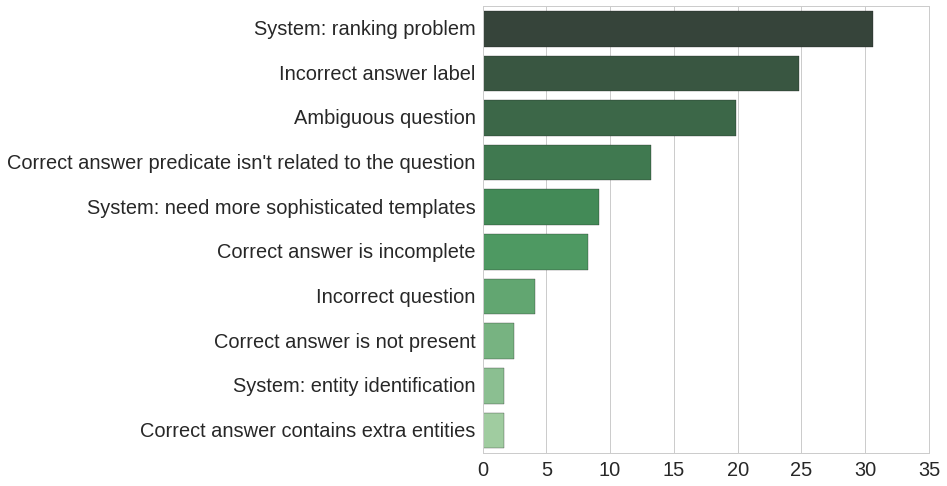
\includegraphics[width=0.6\textwidth]{img/error_analysis}
\caption{Distribution of problems with questions, where Text2KB returns an answer with F1$<$1}
\label{figure:text2kb:error_analysis}
\end{figure}

To get a better insights into the problems that remain, we collected 1219 questions for which Text2KB didn't return completely correct answer, \ie F1 score $<$ 1.
We manually looked through a couple of hundreds of these examples and grouped the problems into several clusters (Figure \ref{figure:text2kb:error_analysis}).

As we can see candidate ranking is still the major problem, and it accounts for $\sim31\%$ of the cases.
The second problem is incorrect ground truth labels (almost 25\% of reported errors).
Another set of questions has incomplete or overcomplete ground truth answer list.
Typical examples are questions asking for a list of movies, books, landmarks, \etc
The ground truth answer usually contains $\sim10$ entities, whereas the full list is often much larger.
This seems to be an artifact of the labeling process, where the answer was selected from the Freebase entity profile page, which shows only a sample of 10 entities, while the rest are hidden behind the ``N values total'' link.
About 20\% of the questions are ambiguous, \ie questions have no strict 1-1 correspondence with any of the predicates and can be answered by multiple ones without any obvious preferences.
For example, the question \textit{``what did hayes do?''} can be answered by profession, occupied position or some other achievements.
Another problem is when there is no predicate that answers the question.
For example, the question \textit{``what do people in france like to do for fun?''} doesn't have a good match among the facts stored in Freebase.
The ground truth entity \texttt{Cycling} comes from the list Olympic sport competitions country participated\footnote{\texttt{olympics.olympic\_participating\_country.athletes}}.

Text2KB components were quite effective in resolving some of the problems.
Web search results helped identify the right question topical entity in a number of cases, \eg \textit{``what did romo do?''} mentions only the last name of the Dallas Cowboys quarterback and the baseline system were unable to map it to the right entity.
Web search results provides more than enough evidence that ``\textit{romo}'' refers to \texttt{Tony Romo}.
However, there are a number of loses, introduced by added unrelated entities.
For example, the entity \texttt{I Love Lucy} was added for the question \textit{``what was lucille ball?''}, because the term \textit{lucy} had high similarity with \textit{lucille}.
A portion of these problems can be fixed by a better entity linking strategy, \eg \cite{SMAPH_ERD:2014}.
An interesting example, when external text resources improved the performance is the question \textit{``what ship did darwin sail around the world?''}.
This is actually a hard question, because the ship entity is connected to the \texttt{Charles Darwin} entity through the ``knownFor'' predicate along with some other entities like \texttt{Natural selection}.
% \footnote{\texttt{user.lindenb.default\_domain.scientist.known\_for}
Thus, the predicate itself isn't related to the question, but nevertheless, the name of the ship \texttt{HMS Beagle} is mentioned multiple times in the web search results, and entity pair model computed from ClueWeb also has high scores for the terms ``ship'' and ``world''.

There are several major reasons for the loses, introduced by features based on external text resources.
Some entities often mentioned together and therefore one of them gets high values of cooccurrence features.
For example, the baseline system answered the question \textit{``when did tony romo got drafted?''} correctly, but since \texttt{Tony Romo} is often followed by \texttt{Dallas Cowboys}, Text2KB ranked the team name higher.
Another common problem with our features is an artifact of entity linking, which works better for names and often skips abstract entities, like professions.
For example, the correct answer to the question \textit{``what did jesse owens won?''} is an entity with the name \texttt{Associated Press Male Athlete of the Year}, which is rarely mentioned or it's hard to find such mentions.
Some problems were introduced by a combination of components.
For example, for \textit{``where buddha come from?''} a topical entity \texttt{Buddhism} was introduced from search results, and it generated \texttt{Gautama Buddha} as one of the answer candidates.
This answer was ranked the highest due to large number of mentions in the search results.

\subsubsection{Summary}
\label{section:factoid:approaches:text2kb:summary}

In summary, in this section we demonstrated that unstructured text resources can be effectively utilized for knowledge base question answering to improve query understanding, candidate answer generation and ranking.
Textual resources can help KBQA system mitigate the problems of matching between knowledge base entities and predicates and textual representation of the question.

Unfortunately, Text2KB doesn't help with the problem of knowledge base incompleteness, \ie our system won't be able to respond to the question, which refers to an entity, a predicate or a fact, which is missing in a KB.
Section~\ref{section:factoid:proposal} describes research I propose to overcome this problem.

% =-=-=-=-=-=-=-=-=-=-=-=-=-=-Text2KB: End=-=-=-=-=-=-=-=-=-=-=-=-=-=-=-=-=-

\section{Proposed Research: Hybrid Question Answering using Text and Knowledge Base Data}
\label{section:factoid:proposal}

Experiments from Section~\ref{section:factoid:approaches:text2kb} demonstrated the effectiveness of unstructured data, such as natural language text, to bridge the lexical chasm between KB concepts and natural language questions.
However, such an approach only works if concepts and facts referred in the question actually exists in KB.
In reality, a big fraction of real user questions cannot be answered using KB data, which is supported by relatively low performance of KBQA systems on general set of factoid questions, such as TREC QA \cite{Sun:2015:ODQ:2736277.2741651}.



\subsection{Method}
\label{section:factoid:proposal:method}

\begin{figure}
\centering
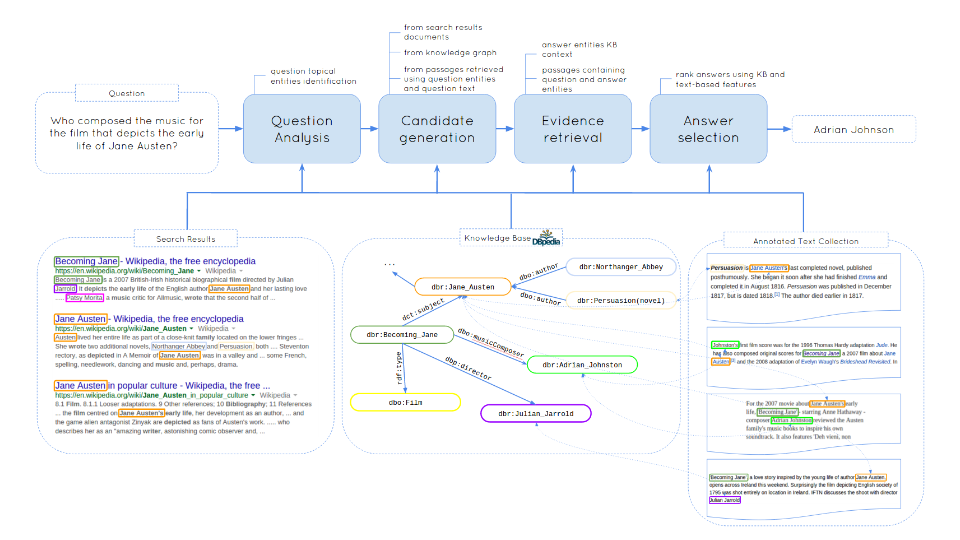
\includegraphics[width=\textwidth]{img/text_and_kb}
\caption{Architecture of a hybrid factoid question answering system, that uses a combination of structured knowledge base and unstructured text data}
\label{figure:factoid:text_kb}
\end{figure}

In this section I propose a novel hybrid QA architecture, that combines unstructured text and structured knowledge base data for joint inference.
Figure \ref{figure:factoid:text_kb} gives a general overview of the proposed system.
The idea is to extend the documents representation with annotations of KB entity mentions, which essentially creates additional edges in the knowledge graph.
These edges connecting KB entities with text fragments can be traversed by a QA system in both directions in order to get more syntactic (from entity to text) or semantic (from text to entity) information.
In addition, text fragments, that mention 2 different entities close to each other can serve as an addition knowledge triple.
Unlike information extraction approaches, however, we don't try to extract the predicate and get rid of all the other information stated in a sentence.
In the proposed approach we are going to use text similarity metrics to retrieve such triples.

The main stages of the proposed QA pipeline are the following (Figure~\ref{figure:factoid:text_kb}):
\begin{enumerate}
\item \textbf{Question analysis}
	\begin{itemize}
	  \item \textbf{Pre-processing}: identify mentions of KB entities in text document collection and index the documents text and mentions in separate fields
  	  \item \textbf{Topical entity identification}: search the text collection using question (or reformulated question \cite{AgichteinLG01}) as a query and use an approach similar to \cite{cornolti2014smaph} to detect question topical entities
    \end{itemize}
  
\item \textbf{Candidate generation}
	\begin{itemize}
	  \item \textbf{Candidate generation from text}: extract candidate answer (or intermediate answer) entities with evidence from the retrieved text documents using existing techniques, e.g. \cite{tsai2015web}.
  	  \item \textbf{Candidate generation from KB}: explore the KB neighborhood of question topical entities and entities extracted from text documents on the previous step
	  \item \textbf{Candidate generation from KB \& Text}: use entity and text index to find entities mentioned near question topical entity and question terms in the document collection
	\end{itemize}
\item \textbf{Evidence retrieval}
    \begin{itemize}
	  \item \textbf{KB evidence extraction}: match neighborhood of answer entities (entity type and other entities) against the question to get additional evidence
      \item \textbf{Text evidence extraction}: estimate the similarity between the collection text fragments mentioning question and answer entities and the question text
    \end{itemize}
\item \textbf{Answer selection}
	\begin{itemize}
	  \item \textbf{Rank candidate}: rank candidate answers using evidence extracted from the KB as well as from text. One particular appealing idea for a ranking model is to estimate $p(q|G_e)$, where $G_e$ is a knowledge subgraph, associated with the current answer candidate. This probability estimates how likely the question could be generated from the knowledge subgraph language model.
    \end{itemize}
\end{enumerate}

As a motivating example, let's consider the following question from the QALD dataset: ``\textit{Who composed the music for the film that depicted the early life of Jane Austen?}''.
Even though it's quite easy to identify the ``\texttt{Jane Austen}'' entity in the question, the knowledge base (dbPedia in this example) cannot help us to determine which movie is being referred to.
However, there are plentiful of documents on the web, that describe the plot of the \texttt{Becoming Jane} movie, and a system can use the proximity of terms from the question \textit{``... depicted early life of Jane Austen''} to the movie entity.
Unfortunately, extracting the name of the composer from these documents is quite challenging, but this task can be easily accomplished by checking the value of the \texttt{musicComposer} property in the knowledge base.
At the end, for each candidate answer entity, we have all the KB information and passages that mention this entity as evidence to help with the correct answer selection.

Essentially, the proposed model is a search based approach, similar to existing information extraction methods for knowledge base question answering~\cite{YaoD14,bastmore:cikm:2015:aquu}, but over the knowledge graph extended with the links to entity mentions in text collections.
In traditional KBQA a special lexicon is used to match terms and phrases in the question to predicates, which essentially represent KB edges.
For text edges I'm planning to use the following two approaches: IR-based methods, in particular recent advances in entity search~\cite{zhiltsov2015fielded,nikolaev2016parameterized}, and neural network joint embeddings of predicates and text fragments~\cite{BordesCW14:emnlp,miller2016key}.

\subsection{Experimentation}
\label{section:factoid:proposal:experiments}

To evaluate the performance of the proposed approach I will compare it against several alternatives on multiple datasets.
The baselines I will compare against include knowledge base question answering system Aqqu~\cite{bastmore:cikm:2015:aquu}, a semantically enriched text-based system QuASE~\cite{Sun:2015:ODQ:2736277.2741651}, a hybrid YodaQA system, designed to be an open source analogue to IBM Watson~\cite{baudivs2015yodaqa} and open question answering approach of A.Fader et al~\cite{Fader:2014:OQA:2623330.2623677}.

Most of the recent work in knowledge base question answering were evaluated on the WebQuestions dataset~\cite{BerantCFL13:sempre}.
This dataset was recently updated to include ground truth semantic parses and many wrong labels were fixed~\cite{yih2016webquestionssp}.
I'm planning to evaluate the system I'm going to built on these datasets.
Since the answers to these questions can be lists, the official evaluation metric is average F1 score over all questions.
However, WebQuestions dataset has its limitations, \eg all the questions are selected so that they could be answered from Freebase.
Furthermore, answers to the question were labeled using entities' Freebase profile pages, which only displays relations in the close proximity to the target entity.
This makes it possible to exploit a small set of templates to generate candidate answer queries.

Traditionally, most of the works in question answering have been evaluated on the TREC QA datasets.
These datasets come with a set of regular expression patterns that can judge an answer as correct or incorrect.
Unfortunately, these patterns aren't complete and researchers often end up re-validating the answers of their systems manually~\cite{Sun:2015:ODQ:2736277.2741651,tsai2015web}.
Unlike most of the previous approaches, however, the proposed system aims at retrieving KB entities as answers of the questions.
Therefore, I will annotate TREC QA datasets with KB entity identifiers of the correct answers.
The baseline systems I mentioned were evaluated of some parts of TREC QA dataset, and I'm going to use reported results instead of reimplementing them.
For my system, I will use ClueWeb12 collection, which was annotated with Freebase entity mentions~\cite{gabrilovich2013facc1}.
The text around mentions will be indexed with Lucene\footnote{https://lucene.apache.org/} open source search engine.
The metrics used for evaluation typically include accuracy and mean reciprocal rank (MRR).

However, TREC QA dataset contains only a couple of thousands of examples, which is relatively small.
As an alternative, I'm designing a new factoid QA dataset, derived from questions posted to Yahoo! Answers CQA website.


\subsubsection{New factoid question answering dataset}
\label{section:factoid:proposal:experiments:dataset}

% \todo{Note to myself: I guess we won't be allowed to make this dataset public as is, because it's derived from Yahoo WebScope dataset.}

Community question answering websites contains hundreds of millions of different questions and corresponding answers, posted by real users.
A fraction of these questions represent factoid information needs.
I'm going to filter a subset of these questions using a set of heuristics or rules.
For example, we can select a subset of QnA pairs with at least one entity in the question and answer, without personal pronouns, words like ``\textit{recommend}'', ``\textit{suggest}'', superlative adjectives like ``\textit{best}'', \etc.
Next this QnA pairs will be further labeled by Mechanical Turk users, who will determine if the questions are indeed factoid and non-subjective and select the actual answer entity from the list of entities, mentioned in the answer text.
The preliminary analysis showed, that from 3.8M QnA pairs from Yahoo! Answers WebScope collection, 80K passed the heuristics filters described above and about 30\% of them are actually good factoid questions.
Examples of questions are: ``\textit{What was James Bond's wife's name?}'', ``\textit{What is the name of the second US astronaut to land on the moon?}'', ``\textit{When was the first "cartoon human" movie?}'', ``\textit{What movie did Joe Pesci describe kids as "YUTS"?}''.
I expect this dataset to contain ~10K real user questions annotated with answer entities, which can be used for future research in question answering in both knowledge base and general factoid question answering.

In my thesis this dataset will be used to further compare performances of the proposed approach versus existing KBQA, text and hybrid systems with open code.

\section{Summary}
\label{section:factoid:summary}

In this section we considered two different ways of combining unstructured and structured data to improve factoid question answering.
Relation extraction from question-answer pairs aims at filling some gaps in KB fact coverage, whereas semantic annotations of text documents provides a way to incorporate information available in unstructured text documents for reasoning along with KB data to improve the performance of factoid question answering.
The experiments proposed in this Chapter will help to answer the question on whether combining structured and unstructured data into a single entity graph is beneficial for the question answering performance compared to text-based, KBQA-based or alternative hybrid approaches.

Factoid questions represent just a part of user information needs. Many problems require more elaborate response, such as a sentence, list of instructions or, in general, a passage of text.
Such questions are usually referred to as non-factoid questions and they will be the focus of the Chapter~\ref{chapter:non-factoid}.

% chap4_nonfactoid.tex
%

\mychapter{Improving Non-factoid Question Answering}
\label{chapter:non-factoid}

\noindent

Even though factoid questions represent a big portion of user information needs, there are many other types of questions, that do not fit into this category, \eg why-questions, how-to questions \etc
For the majority of such questions modern search engines still provide users with ``10 blue links'' only.
Extracting relevant pieces of information from search results is often quite challenging.
With the goal of improving the performance of automatic question answering systems for such generic user information needs in 2015 TREC started a series of LiveQA evaluation campaigns\footnote{http://trec-liveqa.org}.
In TREC LiveQA the task is to develop a real-time system to answer real user questions, that are posted live to Yahoo! Answers\footnote{http://answers.yahoo.com/} community question answering platform.
This chapter describes my experience participating in this shared task and research I propose to do to improve non-factoid question answering.

\section{Problem}
\label{section:non-factoid:problem}

User information needs are very diverse, which is reflected in variety of different types of questions, that people post to community question answering websites~\cite{harper2010question,ignatova2009annotating,liu2008understanding}.
Different types of questions require different type of response, which further complicates the problem of automatic question answering.
For example, procedural how-to questions are usually answered with a list of instructions, causal why-questions require a passage with certain explanations, whereas some recommendation questions could be answered with an option (\eg hotel name) and possibly some supporting statements.

Previous research on non-factoid question answering either focused on a small subset of questions (\eg definition questions~\cite{hildebrandt2004answering}), or considered this as a problem of ranking existing answers in CQA archives, which can be reused to answer new questions~\cite{carmel2000eresponder,Shtok:2012:LPA:2187836.2187939}.
The later strategy of retrieving similar previously posted questions turned out to be quite effective, as it allows a system to return a naturally looking answer in cases when a good match was found.
However, many similar questions are formulated differently, which complicates the retrieval problem, additionally many incoming information needs are still unique and there are simply no similar questions in the archive.
In this case, the system has no other option but to fall back to retrieving potentially relevant passages from regular document collections, such as the web.
The system I developed to participate in TREC LiveQA shared task combines these data sources in a single framework, which selects the answer to return from a single pool of candidate answers.
The problem of selecting best answer sentence received a lot of attention in recent years\footnote{http://aclweb.org/aclwiki/index.php?title=Question\_Answering\_(State\_of\_the\_art)}, and some of this results generalize well to selecting whole passages~\cite{diwang_lstm_2015}.
The candidate ranking module of my system builds on some of these results.
However, individual passages, and even answers to similar questions, often provide just a portion of relevant information a user might want to get.
Therefore, a problem of answer summarization becomes quite important~\cite{liu2008understanding,pande2013summarizing,tomasoni2010metadata}.
In my thesis I'm planning to work on this problem and the proposed research is described later in this chapter.

In section~\ref{section:non-factoid:approach} I will describe a system I developed to participate in TREC LiveQA shared task, which establishes a baseline for future experiments.
Section~\ref{section:non-factoid:proposal} describes the proposed research to improve the performance of non-factoid question answering.

\section{Approach}
\label{section:non-factoid:approach}

% -=-=-=-=-=-=-=-=-=-=-=-= LiveQA : Begin -=-=-=-=-=-=-=-=-=-=-=

In this section, I describe the architecture of the automatic question answering system, which I developed to participate in TREC LiveQA shared task.
The system builds on some existing research on question answering and is based on a combination of CQA archive and web search based approaches.
There are a lot of different types of questions that users post to CQA websites and it is probably beneficial to study them separately.
However, for simplicity the model I built treats all questions in the same way.
My system is based on a single trained model, that ranks a set of extracted answer candidates and returns the top one as the response.
Preliminary analysis of questions and potential answer sources gave an insight that the best data source is answers to similar questions in case they exist and we can find them.
People often have similar tasks and situations which pose same questions.
Therefore, it's frequently the case that a similar question was already asked by someone and potentially even received a good reply and can be reused to answer new questions \cite{Shtok:2012:LPA:2187836.2187939}.
Of course, many questions or their details are unique, which makes it impossible to find a good match from the existing answers.
Therefore I also use web search to generate additional answer candidates.
For non-factoid questions it's harder to use the redundancy of the information on the web, which is exploited very effectively in factoid QA \cite{lin2007exploration}.
The system I developed extracts passages containing question terms from all retrieved web documents independently.
For training I used the publicly available collection of QnA pairs from Yahoo! Answers.
The assumption made was that for each question the answer selected as the ``best answer'' on Yahoo! Answers is indeed the best and should be ranked higher than answers to other questions.
However, taking all other answers is intractable and probably detrimental as almost all of them would be totally unrelated to the subject of the given question.
Therefore, I used search to retrieve a set of similar questions and took their answers as negative examples.
The following chapters describe the QA system in more detail.

\subsection{System architecture}
\label{section:non-factoid:liveqa:architecture}

\begin{figure}
	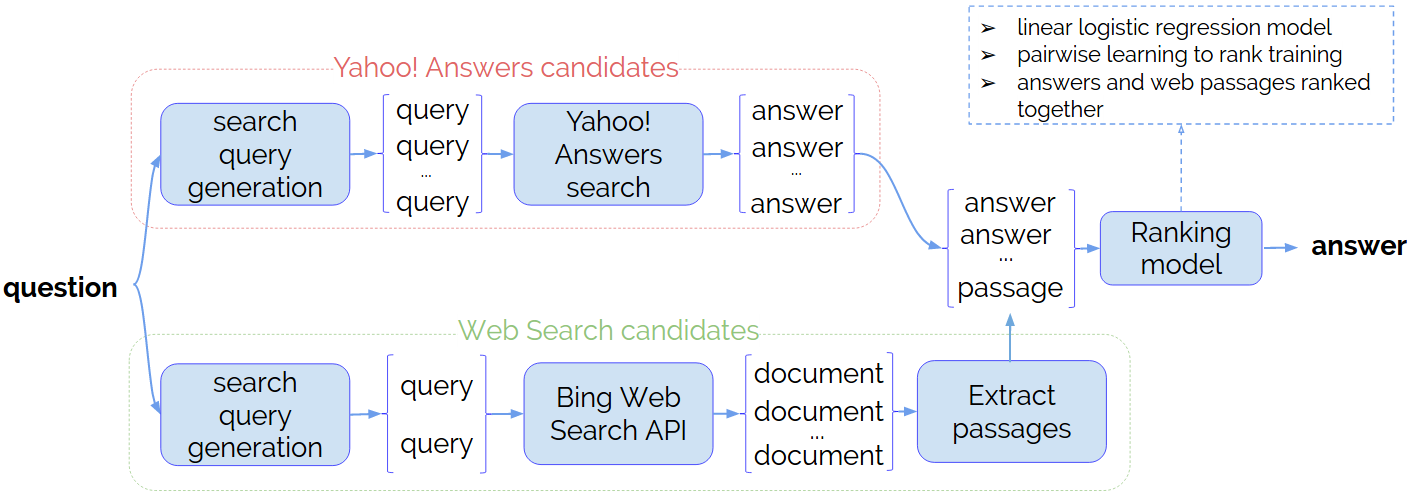
\includegraphics[width=\textwidth]{img/liveqa_qa_model}
	\caption{Architecture of the question answering system I developed to participate in TREC LiveQA shared task}
	\label{figure:non-factoid:liveqa:qa_model}
\end{figure}

The general architecture of our question answering system is presented on Figure~\ref{figure:non-factoid:liveqa:qa_model}.
It uses two primary data sources for generating answer candidates: answers to similar questions from Yahoo! Answers website and documents retrieved using web search. 
All candidates are mixed together, ranked and the top answer is returned.

\subsubsection{Candidate generation}
\label{section:non-factoid:liveqa:architecture:candidates}

Each question issued to a QA system in TREC LiveQA consists of 3 main parts: title, body and category.
For example:

\vspace{3mm}
\begin{tabular}{|p{15cm}|}
\hline
\textbf{Question category}: Astronomy \& Space\\
\textbf{Question title}: Why do people claim the Earth isn't the center of the universe?\\
\textbf{Question body}: Clearly the sun and moon are moving around the Earth otherwise we wouldn't have night and day.\\
\hline
\end{tabular}
\vspace{3mm}

When the QA system receives a question it first generates a set of candidate answers from Yahoo! Answers and regular web search.
To generate a set of candidates the system produces several search queries and issues them to both resources.

To find similar questions and extract the corresponding answers from Yahoo! Answers we use the search functionality already available on the website.
Some questions are very concise while other provide many useful as well as redundant details.
Ideally we want to match as many of them as possible, however, there is a chance that search won't return any results if there are no good matches.
Therefore the system generates a set of search queries of different granularity, issues them all to Yahoo! Answers search and collects top 10 responses from all of them.
Here is the list of queries that our system generates:
\begin{itemize}
	\item Concatenation of question title and question body (with and without stopwords)
	\item Question title only (with and without stopwords)
	\item Question title concatenated with question body and question category
	\item Question title concatenated with the name of the question category
	\item Top 5 terms from question title scored by tf-idf\footnote{Document frequency is computed on WebScope collection of QnA pairs from Yahoo! Answers}
	\item Top 5 terms from question title and body scored by tf-idf
\end{itemize}

For each query and top-10 retrieved questions the system extracts its top answer if provided and puts it into the candidate pool along with some information about the corresponding question and its category.

To extract candidate passages from relevant web documents previous research in factoid question answering have tried query reformulations \cite{Agichtein:2001:LSE:371920.371976} to better match the potential answer text.
However recently \cite{tsai2015web} demonstrated that such reformulations are no longer necessary as search engines have improved the query processing techniques.
Inspired by this observation and considering that retrieving web documents and extracting passages from them is more time consuming, the system issues only 2 web search queries: question title and title concatenated with body. 
I used Bing Web Search API\footnote{http://datamarket.azure.com/dataset/bing/searchweb} and the system downloads top-10 retrieved documents, parses HTML code and extracts the main content text \cite{Kohlschutter_2010}.
Document content is further split into sentences \cite{manning-EtAl:2014:P14-5} and candidates are built by taking contiguous sequences of sentences no longer than the answer character limit\footnote{In the final run the limit was 1000 characters}.
The model only keeps passages that contain at least one non-stopword from the question.
Web search snippets are also included as candidates.

\subsubsection{Candidate ranking}
\label{section:non-factoid:liveqa:architecture:ranking}

A trained linear logistic regression model is used to rank candidate answers, represented with a set of features:
\begin{itemize}
\item answer text statistics: length in character, tokens and sentences, average number of tokens per sentence.
\item Okapi BM25 scores, which consider question title and concatenation of title and body as queries. Term statistics were computed on Yahoo! Answers WebScope dataset. The score is calculated as follows:
\begin{equation*}
\label{equation:bm25}
\text{score}(A,Q) = \sum_{i=1}^{n} \text{IDF}(q_i) \cdot \frac{f(q_i, A) \cdot (k_1 + 1)}{f(q_i, A) + k_1 \cdot (1 - b + b \cdot \frac{|A|}{\text{avg\_al}})}
\end{equation*}
where $f(q_i, A)$ is frequency of term $q_i$ in the answer text, $k_1=1.2$, $B=0.75$ and $avg_al=50$ (average answer length).
\item term matches features: lemmas, part of speech tags of matched terms between the question and answer texts, the fraction of unique question terms matched in the answer, length of the maximum span of matched terms in the answer.
\item number of matched terms between the question title, body and the title of the page from which the candidate answer is retrieved. For Yahoo! Answers the text of the retrieved question is used as title.
\item category match feature for Yahoo! Answers candidates.
\item pairs of lemmas from question and answer texts, that are supposed to bridge the lexical gap between question and answer language.
\item average, minimum and maximum normalized pointwise mutual information (NPMI) scores between pairs of terms from the question and answer texts. The scores are estimated from QnA pairs from Yahoo! Answers WebScope dataset using the following formula:
\begin{equation*}
\begin{split}
\operatorname{npmi}(q_i;a_j) = \frac{pmi(q_i;a_j)}{-\log p(q_i,a_j)}\\
\operatorname{pmi}(q_i;a_j) = \log\frac{p(q_i,a_j)}{p(q_i)p(a_j)} =  \log\frac{p(a_j|q_i)}{p(a_j)}
\end{split}
\end{equation*}
\item QnA pair score from a Long Short Term Memory (LSTM) neural network model, described in Section~\ref{section:non-factoid:liveqa:architecture:training}.
\end{itemize}

The candidate with the highest score is returned as the answer to the question.
If something goes wrong and no candidates were generated or some problem occurred the system returns ``I don't know'' as the default answer.

\subsubsection{Model Training}
\label{section:non-factoid:liveqa:architecture:training}

There are two trained models used in the system: LSTM recurrent neural network based model, which is used as one of the features for the final logistic regression model that scores all candidates and selects the best one as the answer.
I use WebScope Yahoo! Answers dataset\footnote{https://webscope.sandbox.yahoo.com/catalog.php?datatype=l} (different splits are used) to generate training data for both LSTM and ranking model, Figure~\ref{figure:non-factoid:liveqa:model_training} describes the steps I took to build training datasets.

\begin{figure*}
	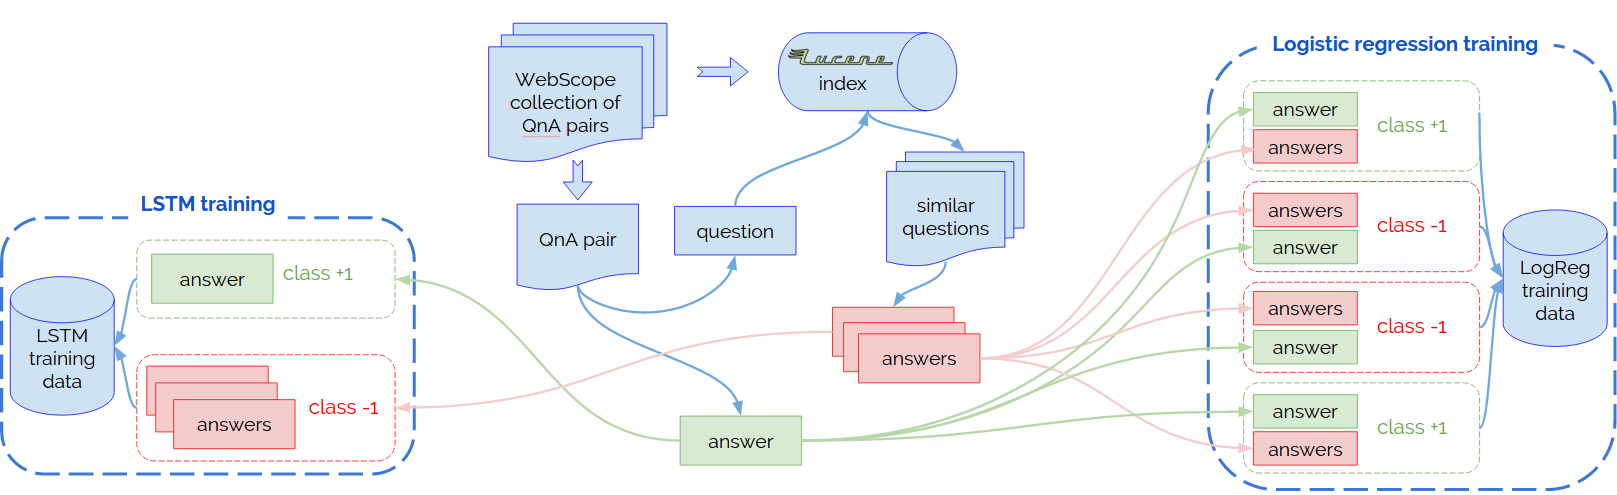
\includegraphics[width=470px]{img/liveqa_model_training}
	\caption{Workflow for generating training datasets for LSTM and answer ranking logistic regression model from the Yahoo! Answers QnA pairs}
	\label{figure:non-factoid:liveqa:model_training}
\end{figure*}

\textbf{LSTM model}.
Deep learning models had a huge success in image and speech problems and showed very promising results in natural language processing and question answering, e.g. \cite{yu2014deep,diwang_lstm_2015} to name a few.
I decided to explore this direction and built a recurrent neural network model to score how well a candidate answers a question.
Long Short-Term Memory (LSTM) \cite{hochreiter1997long} is a particular architecture of recurrent neural networks that helps with the exploding and vanishing gradients problems.
The model I developed reads question and answer tokens and produces a probability score based on a vector representation of a QnA pair.
Figure~\ref{figure:non-factoid:liveqa:lstm_model} shows the structure of the model.

\begin{figure}
	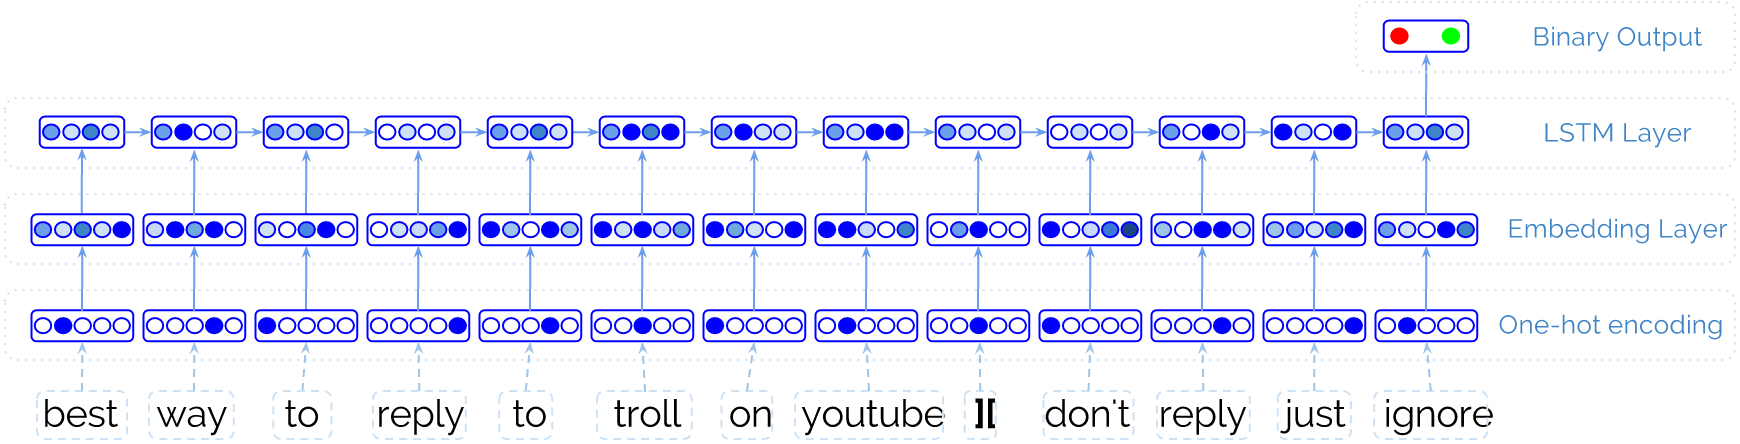
\includegraphics[width=\textwidth]{img/liveqa_qa_lstm}
	\caption{LSTM model for answer scoring. The example shows a QnA pair where the question is ``Best way to reply to trolls on youtube?'' and the answer is ``Don't reply, just ignore''.}
	\label{figure:non-factoid:liveqa:lstm_model}
\end{figure}

Question (title with body) and answer texts are tokenized, punctuation characters are removed and for each token lowercase lemma is taken.
The sequences are limited to 100 elements and concatenated through a sentinel separator character so the model could learn where the question ends and the answer starts.
The hidden state of the model after the whole sequence is processed is used by logistic regression unit to output a probability, that a candidate answers the question well.

To train the model QnA pairs from Yahoo! Answers WebScope dataset were used (we selected a subset of questions from the categories chosen for TREC LiveQA).
Each question and the corresponding best answer was used as a positive training example.
Random negative examples would be too unrelated to the current question, therefore I chose to use answers to similar questions only.
All QnA pairs were indexed with Lucene\footnote{https://lucene.apache.org/} and similar questions were retrieved using the built-in BM25 retrieval model.
For each question and correct answer pair from the dataset 10 similar questions were retrieved and the corresponding answers were used as negative examples for training\footnote{It's true, that some of them can indeed be relevant to the original question}.

The model was implemented using Keras\footnote{http://keras.io} library.
I used an embedding and hidden layers of dimension 128 and the vocabulary size of 1M words.
The model was trained using Adam optimization technique \cite{kingma2014adam} with mini batches of 200 instances for 100 epochs.

\textbf{Logistic regression model}.
The final model that ranks all answer candidates is a linear L2-regularized logistic regression model.
To train the model we used a different split of QnA pairs from Yahoo! Answers WebScope dataset.
For each question the corresponding ``best answer'' is taken as the correct one.
To get a sample of negative examples Lucene index is used again and answers to 10 most similar questions are retrieved.
Different from LSTM model training, here I took a pairwise approach for learning to rank and generated training examples from pairs of different answers to the same question, where one answer is the correct one.
That is, let the current question be $Q$, its ``correct'' answer $A^*$, and retrieved candidates $A_1, ..., A_n$.
Each candidate is represented with a set of features: $f(Q, A^*)$, $f(Q, A_1)$, ..., $f(Q, A_n)$.
For each $i=1..n$ we create two training instances, i.e. class 1: $\langle A^*, A_i\rangle$ and class -1: $\langle A_i, A^*\rangle$.
Each such instance is represented with pairwise differences of features, e.g. $\langle A^*, A_i\rangle: f_{pair}(Q, \langle A^*, A_i\rangle) = f(Q, A^*) - f(Q, A_i)$.
The trained model is linear, therefore if $w(f(Q, A^*) - f(Q, A_i)) > 0$ then $w f(Q, A^*) > w f(Q, A_i)$ and we can rank candidates by the score produced by the model, i.e. $w f(Q, A_i)$.

\subsection{Evaluation}
\label{section:non-factoid:liveqa:evaluation}

From the final run of the system, 1087 questions were judged by the organizers on a scale from 1 to 4:\\
\textbf{4: Excellent} - a significant amount of useful information, fully answers the question\\
\textbf{3: Good} - partially answers the question\\
\textbf{2: Fair} - marginally useful information\\
\textbf{1: Bad} 



% ----------------------------------------

\begin{itemize}
\item : average score over all questions, where scores are translated to 0-3 range. This metric considers ``Bad'', unreadable answers and unanswered questions as having score 0
\item \textbf{succ@i+}: the fraction of answers with score i or greater (i=1..4)
\item \textbf{p@i+}: the number of questions with score i or greater (i=2..4) divided by the number of answered questions
\end{itemize}
Table \ref{table:liveqa-results} provides the results of top 5 teams by average answer score, results for our system and average scores.
Please refer to the \cite{overviewliveqa15} for more details and results of all systems.

\begin{table}
	\caption{Results of the TREC LiveQA evaluation of Emory University QA system and average results of all systems. $\uparrow$ means that results of Emory system in this metric are above average, and $\downarrow$ means that results are below average}
	\label{table:liveqa-results}
	\begin{tabular}{|p{2.5cm}|p{1.7cm}|p{1.3cm}|p{1.3cm}|p{1.3cm}|p{1.3cm}|p{1cm}|p{1cm}|p{1cm}|}
		\hline
		& \# answers & avg score (0-3) & succ@2+ & succ@3+ & succ@4+ & p@2+ &  p@3+ & p@4+ \\
		\hline
		1. CMUOAQA & 1064 & 1.081 & 0.532 & 0.359 & 0.190 & 0.543 & 0.367 & 0.179 \\
		2. ecnucs & 994 & 0.677 & 0.367 & 0.224 & 0.086 & 0.401 & 0.245 & 0.094\\
		3. NUDTMDP1 & 1041 & 0.670 & 0.353 & 0.210 & 0.107 & 0.369 & 0.219 & 0.111\\
		4. RMIT0 & 1074 & 0.666 & 0.364 & 0.220 & 0.082 & 0.369 & 0.223 & 0.083\\
		5. Yahoo-Exp1 & 647 & 0.626 & 0.320 & 0.211 & 0.095 & 0.538 & 0.354 & 0.159\\
		\hline
		7. Emory & 884$\downarrow$ & 0.608$\uparrow$ & 0.332$\uparrow$ & 0.190$\uparrow$ & 0.086$\uparrow$ & 0.408$\uparrow$ & 0.233$\uparrow$ & 0.106$\uparrow$\\
		\hline
		Average results & 1007 & 0.467 & 0.262 & 0.146 & 0.060 & 0.284 & 0.159 & 0.065\\
		\hline
	\end{tabular}
\end{table}

The metric succ@1+ shows the fraction of questions for which a readable answer was returned by the system.
A lower score in this metic means that my system didn't return an answer in time in almost 20 \% of the cases.
A part of the problem is caused by several technical issues, that appeared on the day of the evaluation run.
Due to one of them LSTM model didn't provide any score for a significant fraction of submitted questions, and the other problem made the whole system unresponsive for a couple of hours.
Nevertheless, the overall results look promising and I will make a more thorough analysis of the system performance for the final version of the paper.

The absolute values of the performance metrics demonstrate a great room for improvement as our system was able to return partial or good answer only in 23\% of the cases (prec@3+) when the answer was returned.
And for 60\% of the questions the answer doesn't contain any useful information.


\subsection{Analysis}
\label{section:non-factoid:liveqa:analysis}

In this section we will answer some of the questions about the performance of different system components and their relative importance.

The first question, that we are going to study is the relative effectiveness of web passages and answers to previously posted questions for answering new questions.
As Figure~\ref{figure:non-factoid:liveqa:answer_source_pie} shows, almost half of all answers returned by my system were generated from Yahoo! Answers.
In $\sim$21\% of the cases our system didn't return any results\footnote{This happened mainly due to a couple of technical issues that made our system unresponsive for quite some time}, and in the rest $\sim$31\% of the cases a passage from a web page was returned as the answer.
I further looked into the domains of the web pages used to generate the answer and noticed, that many more were extracted from other community question answering websites and forums.

\begin{figure}
	\centering
	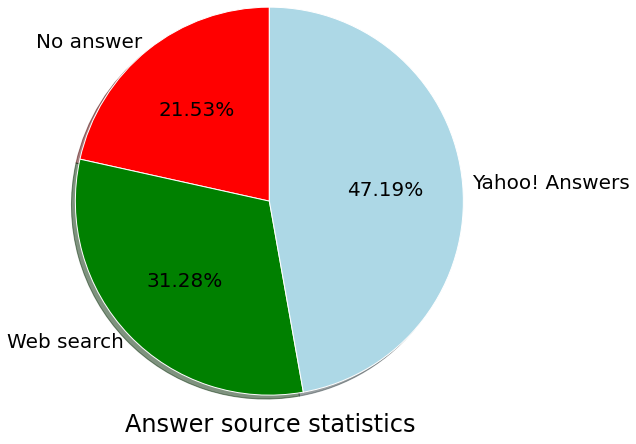
\includegraphics[width=0.5\textwidth]{img/liveqa_answer_source}
	\caption{Distribution of sources for answers returned by our system}
	\label{figure:non-factoid:liveqa:answer_source_pie}
\end{figure}

\begin{figure}
	\centering
	\begin{subfigure}[b]{0.38\textwidth}
		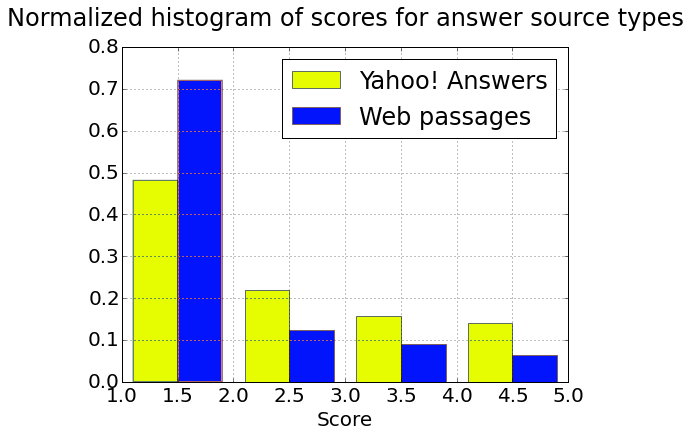
\includegraphics[width=\textwidth]{img/liveqa_answer_source_scores}
		\caption{Histogram of qrel scores}
		\label{figure:non-factoid:liveqa:answer_source:scores}
	\end{subfigure}
	\begin{subfigure}[b]{0.6\textwidth}
		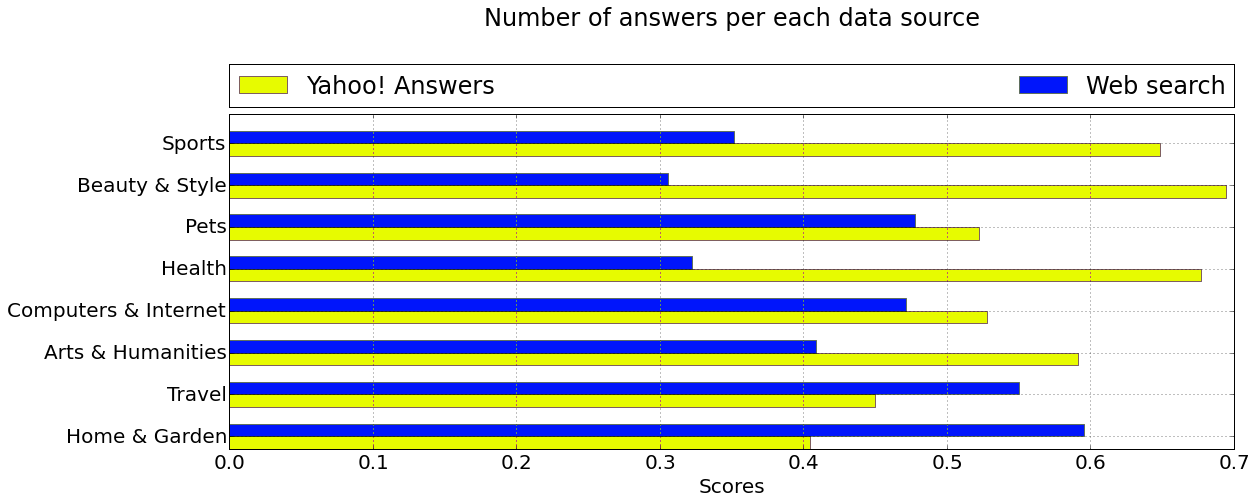
\includegraphics[width=\textwidth]{img/liveqa_answer_source_by_category}
		\caption{Average scores of answers from Yahoo! Answers and web passages for different categories}
		\label{figure:non-factoid:liveqa:answer_source:category}
	\end{subfigure}
	\caption{Comparison of web passages and Yahoo! Answers as candidate sources}
	\label{figure:non-factoid:liveqa:answer_source}
\end{figure}

The quality of answers generated from passages built from web search results are lower on average compared to Yahoo! Answers candidates.
Figure~\ref{figure:non-factoid:liveqa:answer_source} shows the distribution of scores for each of our data sources.
Some categories were harder than the other \cite{Agichtein15:liveqa} and as we see on Figure~\ref{figure:non-factoid:liveqa:answer_source:category} in some cases web passages were actually more effective than answers to previously posted questions.

\begin{figure}
	\centering
	\begin{subfigure}[b]{0.49\textwidth}
		\centering
		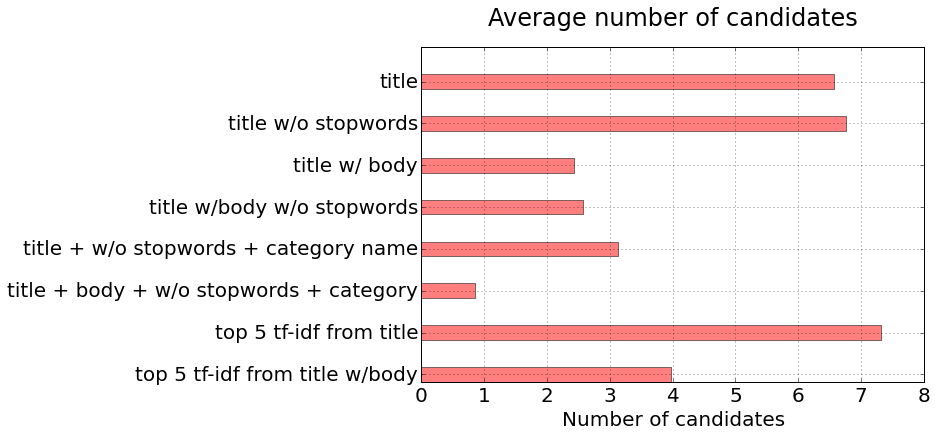
\includegraphics[width=\textwidth]{img/liveqa_query_candidate_count}
		\caption{Average number of candidates}
		\label{figure:non-factoid:liveqa:analysis:query_generation:count}
	\end{subfigure}
	\begin{subfigure}[b]{0.49\textwidth}
		\centering
		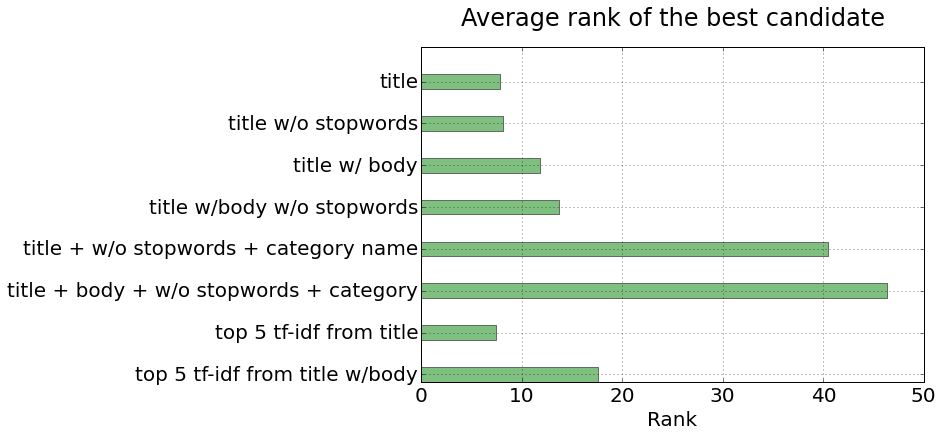
\includegraphics[width=\textwidth]{img/liveqa_query_candidate_bestrank}
		\caption{Average rank (according to our ranking model) of the best candidate}
		\label{figure:non-factoid:liveqa:analysis:query_generation:rank}
	\end{subfigure}
	\caption{Comparison of different query generation strategies for Yahoo! Answers similar questions search}
	\label{figure:non-factoid:liveqa:analysis:query_generation}
\end{figure}

The next question, that we analyze is the effectiveness of search query generation strategies.
Figure~\ref{figure:non-factoid:liveqa:analysis:query_generation} plots average number of candidates and the position of the best candidate retrieved by each of the question generation strategies.
The longer the search query the less results it retrieved, which is expected, and the lower the quality of the candidates.
As a result, in half of the cases the answer returned by our system was retrieved using just top 5 highest IDF terms as the query\footnote{The same candidate is often also retrieved by other queries}.
For web search we only used 2 query generation strategies, namely question title and concatenation of title with body.
Analogously, concatenation of title with body query had lower quality and more often returned few or no results.

Figure~\ref{figure:non-factoid:liveqa:features} demonstrates a plot of importances of different features in our answer ranking linear logistic regression model.
The feature with the highest weight is category match, but we should note, that this feature is overfitted to the way we build training set (category of the correct answer always matched the category of the question).
The next most useful feature is the cosine similarity between the page title (or question text for Yahoo! Answers) and the current question, followed by BM25 score, number of matched verbs, etc.

\begin{figure}
	\centering
	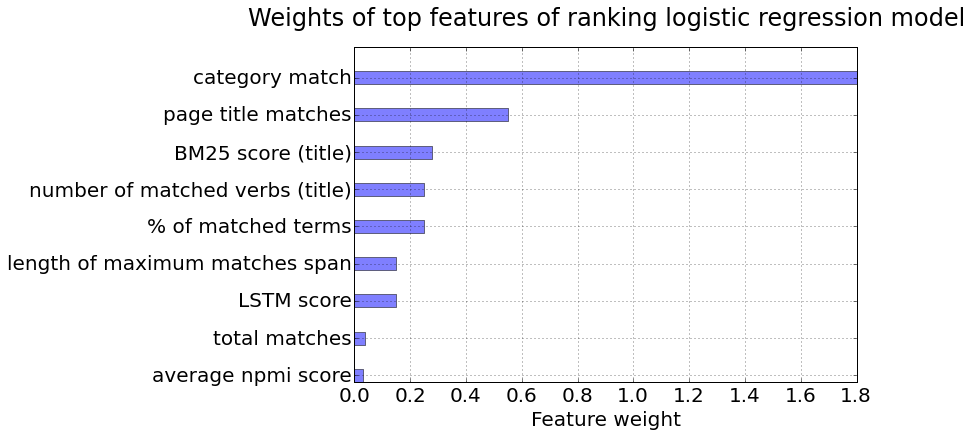
\includegraphics[width=0.6\textwidth]{img/liveqa_features}
	\caption{Weights of features in answer ranking logistic regression model}
	\label{figure:non-factoid:liveqa:features}
\end{figure}

I also looked through a small sample of our answers manually.
There are a number of typical problems, and one of them is the lack of good question semantic similarity measure.
E.g. the question \textit{``Is there a section fro the subject of writing''} in the \texttt{Books \& Authors} category retrieved a question \textit{``I can't write in the To: Cc: Subject: section''} from the \texttt{Yahoo Mail} category.
Even though the questions have many terms in common, they are obviously semantically unrelated.
Therefore, in future we need to focus more on better question similarity measures.

Answer doesn't have to have many words in common with the question.
On the contrary, the maximum possible term overlap will be if a candidate is just a copy of the answer.
This was one of the problems for answers, retrieved from the web search results.
The way we used to generate the training data didn't include such ``artificial'' cases, however, they are pretty common in practice.
For example, in a number of cases the answer our system chose came from a forum post and instead of selecting the answer posts, the system ranked the question post higher as it had more term matches.
The winning CMU team addressed this issue by considering answer-clue pairs, where the clue is supposed to match the question text and the former answers the question.
We plan to explore a similar strategy.

\subsection{Further improvements for TREC LiveQA 2016}
\label{section:non-factoid:liveqa:improvements}

TREC LiveQA 2016 task was run on May 31, and I made a few improvements to my system.
One of the major quality loss in my previous system was due to random crashes, which resulted in no response for more than 200 questions.
This year I changed the architecture of the system to make it more reliable and make sure the answer is returned in time.

Next, as analysis of the previous year track has revealed, many of answers generated using regular web search still came from different community question answering websites.
However, the system didn't treat such pages differently from regular documents and didn't extract additional meta-data, such as the question text, \etc.
Therefore, for LiveQA 2016 I decided to extend a set of data sources and in addition to Yahoo! Answers I added separate candidate generation pipelines for Answers.com and WikiHow.com.
For these verticals the system uses the search engine built into the platforms, and extracts answers along with the corresponding question meta-data.

The other improvements target the candidate answer ranking module of the system.
I've extended a set of features representing each candidate answer to include the following:
\begin{itemize}
	\item Percentage of the terms in the answer, that are not matched against the question. This features aim at estimating the new information in the answer. The previous system often selected answer that simply repeated the question.
	\item N-gram matches features: fraction of 1,2-3-grams from the question title, body that overlaps the n-grams from the answer text
	\item All term match features were computed for related question and body. More specifically, additionally to taking the answer text itself, we added features that compute similarity scores between the current question and retrieved question (title and body). For candidates, generated from regular web documents we tool the title of the page as question title, and the previous paragraph in text as body.
\end{itemize}

Additionally, I replaced the logistic regression ranking model with LambdaMART~\cite{burges2010ranknet}, as implemented in RankLib library\footnote{https://people.cs.umass.edu/~vdang/ranklib.html}.
Unlike the previous year, when training data in a usual sense didn't exist, in 2016 we had relevance judgments from previous campaign.
To train the LambdaMART model I took this data and scraped the original web pages to get meta-information and generate all the features for the candidates.
Using this data I trained the model to optimize NDCG metric.
The results of the evaluation are not available at the moment.

\subsection{Summary}
\label{section:non-factoid:liveqa:summary}

The pilot year of TREC LiveQA establishes a very good baseline for the future of non-factoid question answering.
It confirmed that the task itself is quite challenging as only $\sim$35\% of the questions returned by the winning system had a score of 3 or higher, and there is still a big gap between in the quality of human and machine answers.
It will be exciting to see the next version of the task next year, and how the participants will build on this year approaches.


% -=-=-=-=-=-=-=-=-=-=-=-= LiveQA : End -=-=-=-=-=-=-=-=-=-=-=-=-

\section{Proposed Research}
\label{section:non-factoid:proposal}

The results of TREC LiveQA 2015 established a baseline performance of automatic non-factoid question answering systems, and shed some light on typical problems and future research directions.
For my thesis I'm proposing to focus on one of these problems, \ie answer summarization.
The existing research typically follows an extractive summarization approach, and explores different answer sentences ranking strategy to either shorten the answer, cover multi-intent questions or to improve diversity~\cite{chan2012community,zhaochun_sparsecoding_2016}, and less attention is paid to the overall quality and readability of summarized answer text.

For my thesis I propose to capitalize on the recent successes of deep learning for natural language processing and apply some of the techniques on the new problem of answer summarization.
Section~\ref{section:non-factoid:proposal:method} describes the proposed methodology in more details.

\subsection{Method}
\label{section:non-factoid:proposal:method}

Distributed representations for words~\cite{mikolov2013distributed,pennington2014glove} and longer phrases~\cite{le2014distributed,kiros2015skip} opened up a new era in natural language processing and information retrieval.
Using distributed representations or embeddings one can simply calculate the similarity between words or sentences using various distance metrics in the embeddings space.
Such representations made it possible to train end-to-end models for various NLP tasks, which reach or outperform existing state-of-the-art models~\cite{collobert2011natural}.

Text summarization isn't an exception, and recently a number of different architectures were proposed for both more traditional extractive~\cite{kaageback2014extractive} as well as abstractive summarization~\cite{rush-chopra-weston:2015:EMNLP,chopraabstractive16}.
In answer summarization we are dealing with multiple different piece of text, therefore it's more related to the problem of multi-document summarization~\cite{cao2015ranking}.
However, unlike document summarization, here we have a notion of the question and some answer candidates (if not the majority) might be totally irrelevant to the question and not worth including overall.

\begin{figure}
	\centering
	\begin{subfigure}{0.8\textwidth}
		\centering
		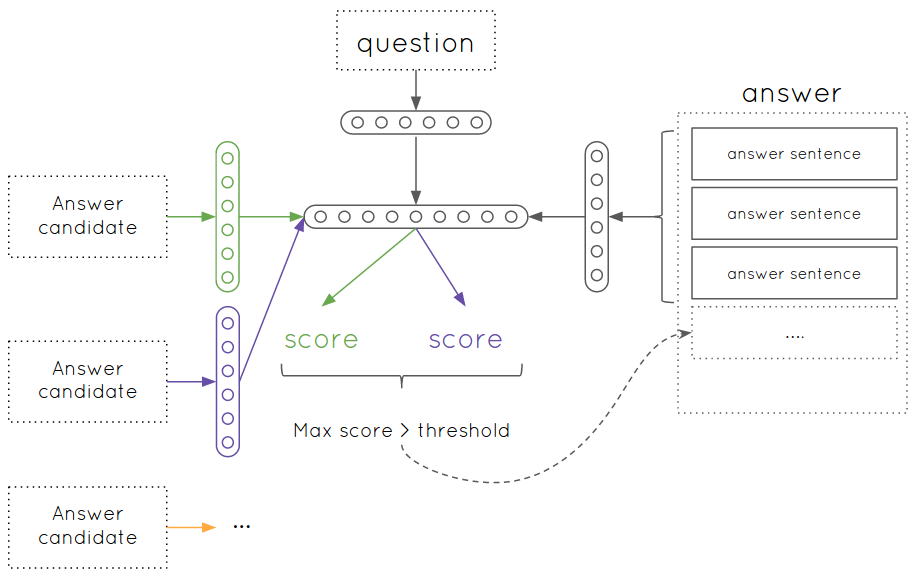
\includegraphics[width=\textwidth]{img/answer_summarization_model}
		\caption{Extractive summarization}
		\label{figure:non-factoid:proposal:model:extractive}
	\end{subfigure}
	
	\begin{subfigure}{0.8\textwidth}
		\centering
		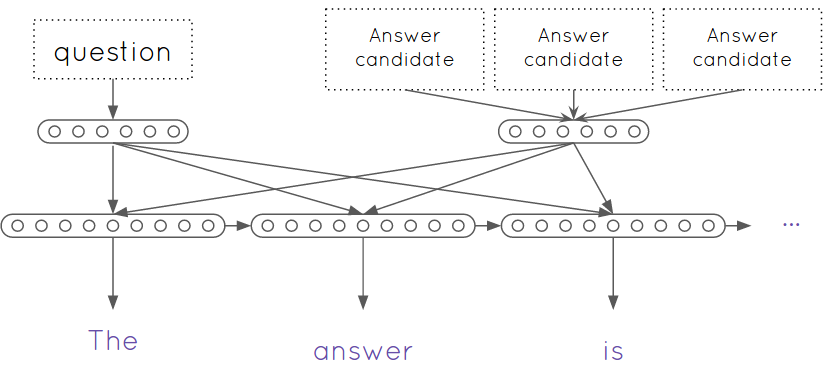
\includegraphics[width=\textwidth]{img/answer_summarization_model_abstractive}
		\caption{Abstractive summarization}
		\label{figure:non-factoid:proposal:model:abstractive}
	\end{subfigure}
	\caption{The architecture of the proposed answer summarization models}
	\label{figure:non-factoid:proposal:model}
\end{figure}

The schematic of the models I propose to implement for answer summarization is depicted on Figure~\ref{figure:non-factoid:proposal:model}.

On each step of the extractive summarization the model takes 3 kinds of inputs: embedding of the question, already constructed summary and answer candidate.
Embeddings of the question and already constructed summaries can be obtained using the attention mechanism~\cite{xu2015show} to focus the model on specific parts of the input.
The idea of abstractive summarization model is based on the sequence to sequence attention-based models, and similar in architecture to the works of Sumit Chopra and Alexander Rush~\cite{chopraabstractive16,rush-chopra-weston:2015:EMNLP}.

\subsection{Experimentation}
\label{section:non-factoid:proposal:experiments}

Since the problem of answer summarization isn't new, there are some datasets already available and several benchmark results exists.
For my experiments I'm planning to use the dataset of M.Tomasoni and M.Huang~\cite{tomasoni2010metadata}, which was constructed based on Yahoo! Answers archive and manually generated gold summaries.
Another relevant dataset, constructed for the task of novelty-based answer reranking was recently released by Adi Omari et al~\cite{omari2016novelty}.
In this dataset human annotators extracted nuggets of different aspects for the same question, and therefore its possible to judge the relevance of each of the answer with respect to these nuggets.
The paper establishes certain baselines for the task of answer reranking using diversity-aware ranking metrics.
Since each answer might contain a lot of redundant information, summarization should allow us to increase the diversity of the answer text given the same length limit.

However, in these dataset the answer candidates were taken from community generated answers to each question, and therefore on average they are relevant.
To test the model on more realistic scenario of automatic question answering, I'm planning to reuse the candidate answers with relevance labels from TREC LiveQA datasets.
The available answer labels can automatically be used to estimate the relevance of individual sentences, extracted from the dataset, and the overall quality of the answers will be judged manually using crowdsourcing.

\section{Summary}
\label{section:non-factoid:summary}

This chapter focus on the problem of improving the performance of non-factoid question answering system.
The system I developed participated in both TREC LiveQA 2015 and 2016 shared tasks, which allowed me to test certain ideas and discover directions for future improvements.
For my thesis I decided to focus on the problem of answer summarization, and proposed extractive and abstractive summarization models, based on recent developments in the field of neural networks.

However, no matter how well an automatic system performs, there will be cases, when it is unable to generate a good response to a user question.
In such cases, computers can ask for help, which would lead to a hybrid human-computer question answering systems.
Chapter~\ref{chapter:crowdsourcing} focuses on the idea of crowdsourcing for realtime question answering.

% chap5_crowdsourcing.tex
%

\mychapter{Crowdsourcing for Real-time Question Answering}
\label{chapter:crowdsourcing}

\noindent

\section{Problem}
\label{section:crowdsourcing:problem}

Despite the progress in automatic question answering, existing systems are still far from being able to handle every human question.
For example, the winning system in TREC LiveQA 2015 shared task were able to return a good or excellent answer to less than 40\% of the questions.
And overall, according to the TREC LiveQA 2015 assessor scores, for 12.6\% of the questions none of the 21 participating systems produced even moderately useful answer, and for 30\% a good or better response.
This can happens for multiple different reasons, \eg a question is ill formulated, available data sources does not contain any relevant information, a system fails to retrieve or rank good answer candidates, \etc
As conversational agents become more popular, QA systems are increasingly expected to handle such complex questions, and to do so in (nearly) real-time, as the searcher is unlikely to wait longer than a minute or two for an answer.

One way to overcome the above mentioned challenges in complex question answering is to develop a hybrid human-computer question answering system, which could consult a crowd of workers in order to generate a good response to the user question.
This section provides some preliminary results and proposed research in crowdsourcing for real-time question answering.
Part of the described results was published at Human-Computer Question Answering workshop at NAACL 2016 conference~\cite{savenkov_crowdsourcing2016a}, and another will appear as a full paper titled ``CRQA: Crowd-powered Real-time Automated Question Answering System'' on HCOMP 2016 conference~\cite{savenkov_crqa2016}.

\section{Approach}
\label{section:crowdsourcing:approach}

In this section I explore two ways crowdsourcing can assist a question answering system that operates in (near) real-time: by providing answer {\em validation}, which could be used to filter or re-rank the candidate answers, and by {\em creating} the answer candidates directly.
First, we study if crowd workers can quickly and reliably judge the quality of the proposed answer candidates, and if it is possible to obtain reasonable written answers from the crowd within a limited amount of time.
Then, we present CRQA, a crowd-powered, near real-time automated question answering system for complex informational tasks, that incorporates a crowdsourcing module for augmenting and validating the candidate answers.
The crowd input, obtained in real-time, is integrated into CRQA via a learning-to-rank model, to select the final system answer.
Our large-scale experiments, performed on a live stream of real users questions, show that even within a one minute time limit, CRQA can produce answers of high quality.

More specifically, in this section we answer the following questions:
\begin{enumerate}
\item Can crowdsourcing be used to judge the quality of answers to non-factoid questions under a time limit?
\item Is it possible to use crowdsourcing to collect answers to real user questions under a time limit?
\item How does the quality of crowdsourced answers to non-factoid questions compare to original CQA answers, and to automatic answers from TREC LiveQA systems?
\item Can crowdsourcing be used to improve the performance of a near real-time automated question answering system?
\item What is the relative contribution of candidate answer ratings and answers provided by the workers to the overall question answering performance?
\item What are the tradeoffs in performance, cost, and scalability of using crowdsourcing for real-time question answering?
\end{enumerate}

To answer the first three questions, we conducted a series of crowdsourcing experiments using the Amazon Mechanical Turk platform\footnote{http://mturk.com}.
We used questions from the TREC LiveQA 2015 shared task, along with the system answers, rated by the NIST assessors\footnote{https://sites.google.com/site/trecliveqa2016/liveqa-qrels-2015}.
The questions for the task were selected by the organizers from the live stream of questions posted to the Yahoo! Answers CQA platform on the day of the challenge (August 31, 2015).
For these questions we also crawled their community answers, that were eventually posted on Yahoo! Answers\footnote{As the answer we took the top question, which was selected as the ``Best answer'' by the author of the question or by the community.}.

\subsection{Crowdsourcing for time-constraint answer generation and validation}
\label{section:crowdsourcing:approach:experiments}

To check if crowdsourcing can be used to judge the quality of answers under a time limit, we asked workers to rate answers to a sample of 100 questions using the official TREC rating scale:
\begin{enumerate}
\item Bad - contains no useful information
\item Fair - marginally useful information
\item Good - partially answers the question
\item Excellent - fully answers the question
\end{enumerate}

\begin{figure*}
\centering
\begin{subfigure}[b]{0.49\textwidth}
\centering
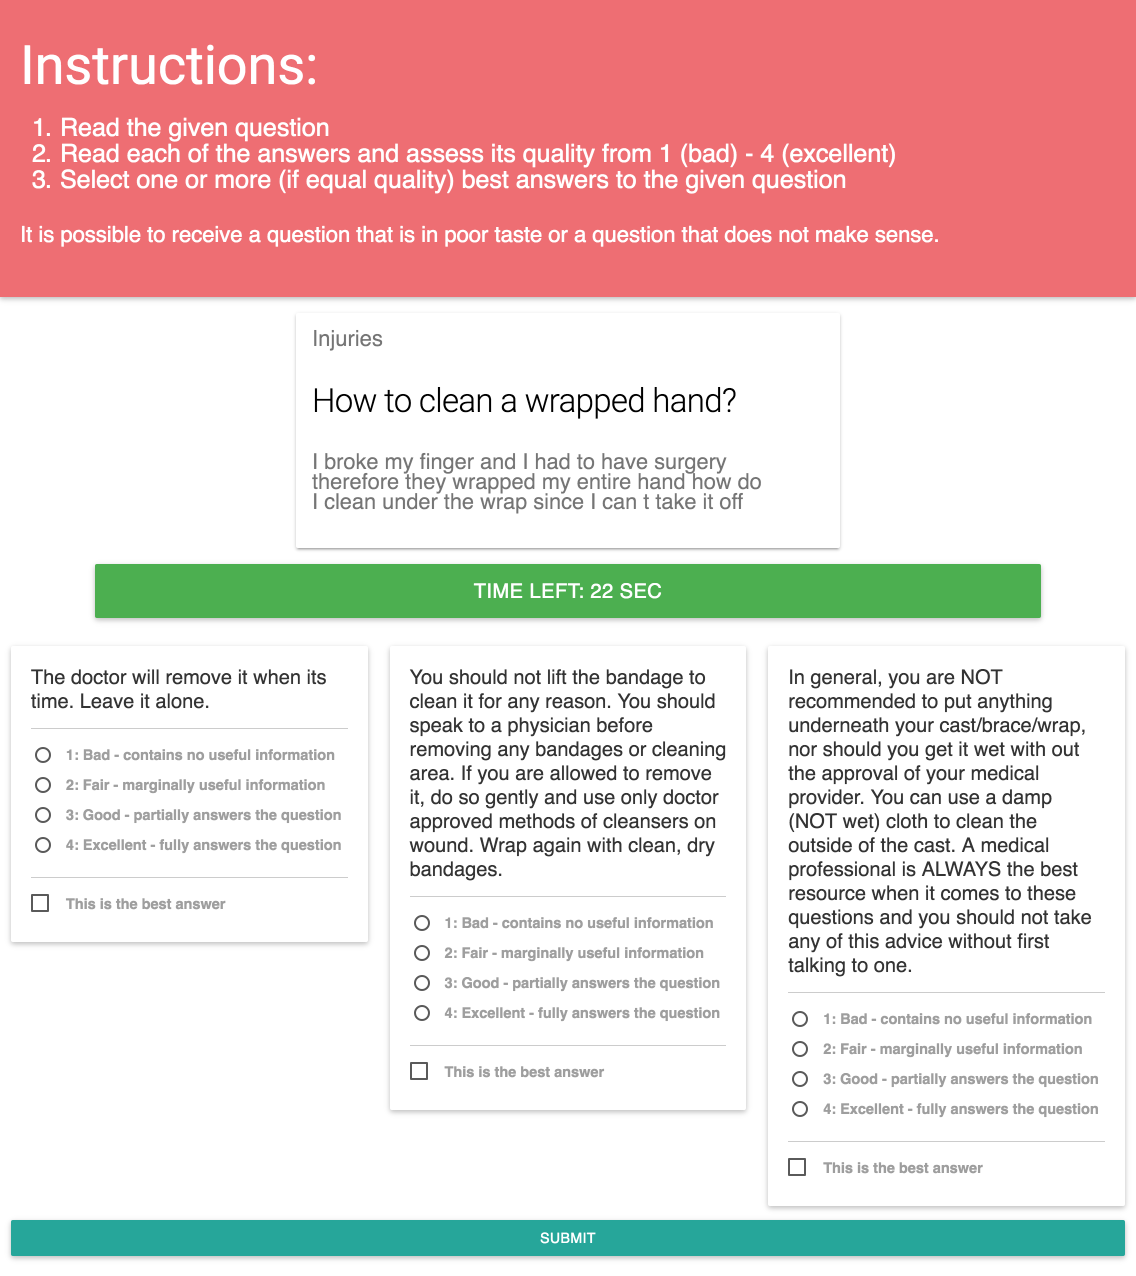
\includegraphics[width=\linewidth]{img/validation_screenshot}
\caption{Answer validation form}
\label{figure:crowdsourcing:interfaces:validation}
\end{subfigure}
\begin{subfigure}[b]{0.49\textwidth}
\centering
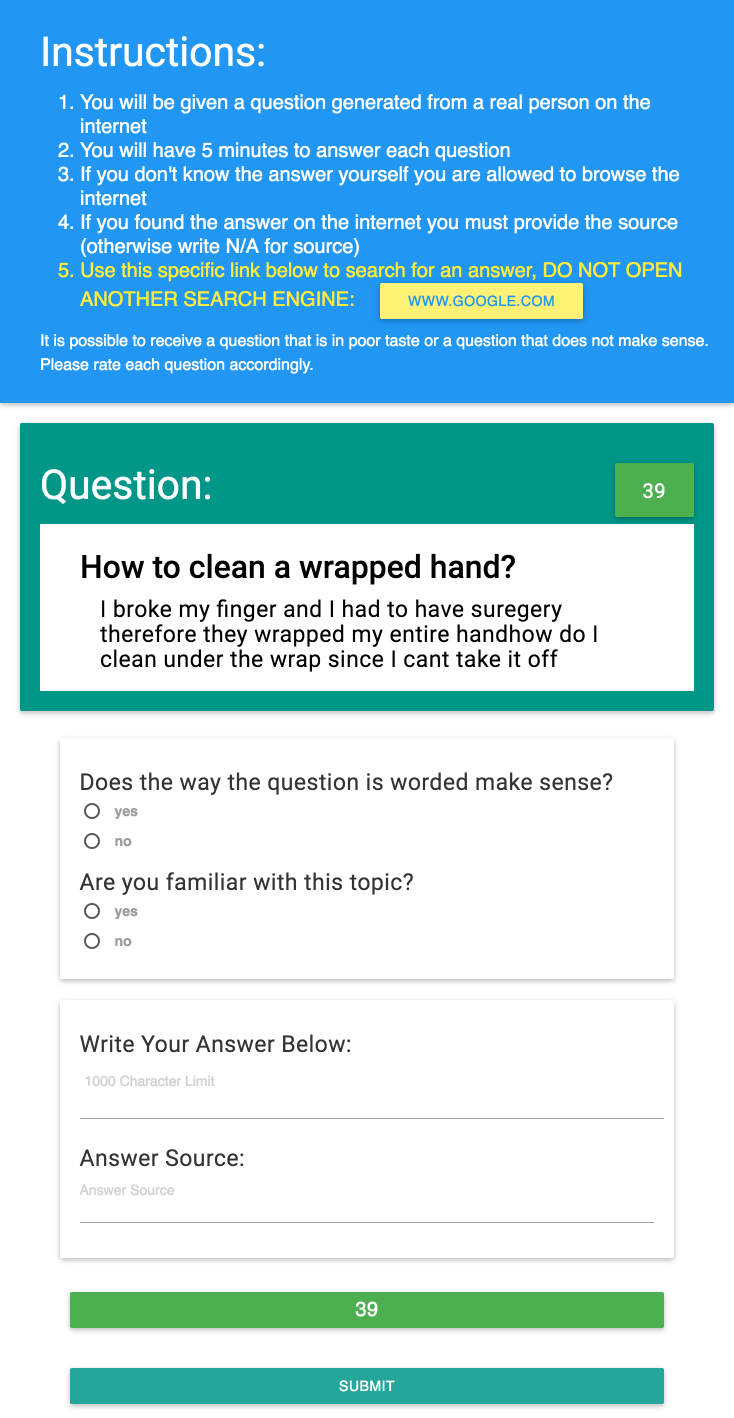
\includegraphics[width=0.9\linewidth]{img/answering_screenshot}
\caption{Answer crowdsourcing form}
\label{figure:crowdsourcing:interfaces:answer}
\end{subfigure}

\caption{Crowdsourcing user interfaces}
\label{figure:crowdsourcing:interfaces}
\end{figure*}

We chose to display 3 answers for a question, which were generated by three of the top-10 automatic systems from TREC LiveQA 2015 evaluation \cite{overviewliveqa15}.
To study the effect of time pressure on the quality of judgments we split participants into two groups. One group made their assessments with a 1 minute countdown timer shown to them, while the other could complete the task without worrying about a time limit.
Within each group, we assigned three different workers per question, and the workers were compensated at a rate of \$0.05 per question for this task.

\subsubsection{Answer validation experiment}
\label{section:crowdsourcing:approach:experiments:validation}

The interface for collecting answer ratings is illustrated in Figure \ref{figure:crowdsourcing:interfaces:validation}\footnote{The screenshots show the final state of the form, as we describe later in this sections fields were unhidden step-by-step for proper timing of reading, answering and validation}.
On top of the interface workers were shown the instructions on the task, and question and answers were hidden at this time.
They were instructed to read the question, read the answers, and rate each answer's quality on a scale from 1 (Bad) to 4 (Excellent), and finally choose a subset of candidates that best answer the question.
Upon clicking a button to indicate that they were done reading the instructions, the question, a 60 second countdown timer and 3 answers to the question appeared on the screen.
At the 15 second mark the timer color changed from green to red.
In the experiments without time pressure the timer was hidden, but we still tracked the time it took for the workers to complete the task.

At the end, we collected 6 ratings (3 with and 3 without time pressure) for each of three answers for a sample of 100 questions, which makes it a total of 1800 judgments.
Each answer also has an official NIST assessor rating on the same scale.
Figure \ref{figure:crowdsourcing:score_correlation} shows correlation between official NIST assessor relevance judgments and ratings provided by our workers.
The Pearson correlation between the scores is $\rho=0.52$.
The distribution of scores shows that official assessors were very strict and assigned many extreme scores of 1 or 4, whereas mechanical turk workers preferred intermediate 2s and 3s.
The results did not show any significant differences between experiments with and without time pressure.
Figure \ref{figure:crowdsourcing:validation_time} shows that even though the median time to rate all three answers is around 22-25 seconds in both experiments, the upper bound is significantly lower in the experiment with the time pressure.

\begin{figure}
	\centering
	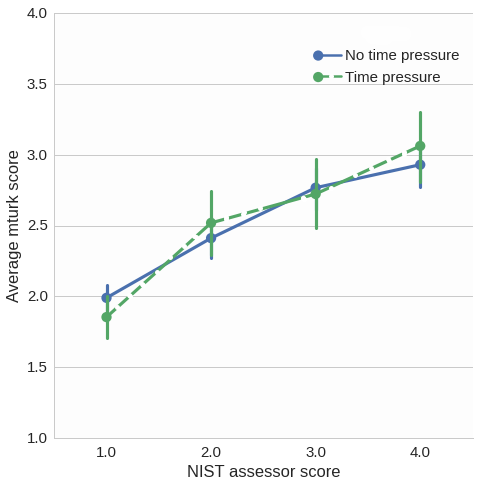
\includegraphics[width=0.35\textwidth]{img/score_correlation}
	\caption{Correlation between NIST assessor scores and crowdsourced ratings with and without time limit on the work time}
	\label{figure:crowdsourcing:score_correlation}
\end{figure}

\begin{figure}
	\centering
	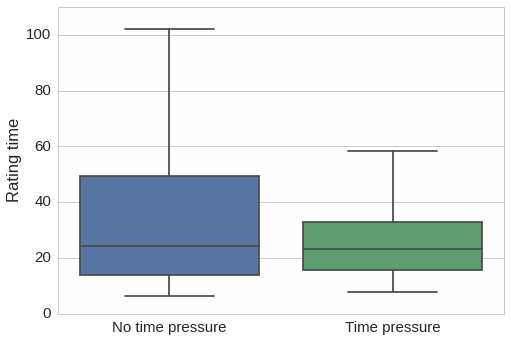
\includegraphics[width=0.4\textwidth]{img/validation_time}
	\caption{Box plot of answer rating time with and without time pressure}
	\label{figure:crowdsourcing:validation_time}
\end{figure}


Therefore, we conclude that in general we can trust crowdsourced ratings, and on average one minute is enough to judge the quality of three answers to CQA questions.

\subsubsection{Answer generation experiment}
\label{section:crowdsourcing:approach:experiments:generation}

In another experiment, designed to check whether crowd workers can provide an answer to a given question within a limited amount of time, we asked different workers to answer the questions from TREC LiveQA 2015.
We split the workers into two groups and displayed a one minute countdown timer for one of them.
We left a grace period and let the workers submit their answers after the timer had run out.
The workers received a \$0.10 compensation for each answer.
The form for answer crowdsourcing is shown in Figure \ref{figure:crowdsourcing:interfaces:answer}, and similar to the answer rating form, it starts with a set of instructions for the task.
We let the users browse the internet if they were not familiar with the topic or could not answer the question themselves.
To prevent them from finding the original question on Yahoo! Answers, we included a link to Google search engine with a date filter enabled\footnote{https://www.google.com/webhp?tbs=cdr:1,cd\_max:8/30/2015}.
Using this link, workers could search the web as it was on 8/30/2015, before TREC LiveQA 2015 questions were posted and therefore workers were in the same conditions as automatic systems on the day of challenge\footnote{The ranking of search results could be different on the day of the challenge and for our workers}.
Initially, the question was hidden for proper accounting of question-reading and answering times.
Upon clicking a button to indicate that they were done reading the instructions, a question appeared along with a button, which needed to be clicked to indicate that they were done reading the question.
After that, the answering form appears, it contained four fields:
\begin{enumerate}
\item Does the question make sense: ``yes'' or ``no'' to see if the question was comprehensible
\item Are you familiar with the topic: A yes or no question to evaluate whether the worker has had prior knowledge regarding the question topic
\item Answer: the field to be used for the user's answer to the given question
\item Source: the source used to find the answer: URL of a webpage or NA if the worker used his own expertise
\end{enumerate}

At the end, we collected 6 answers (3 with and without time pressure) for each of the 1087 LiveQA'15 questions.
Since we have answers from different sources, let's introduce the following notations:
\begin{itemize}
	\item \textit{Yahoo! Answers} - answers eventually posted by users on Yahoo! Answers for the original questions
	\item \textit{Crowd} - answers collected from Mechanical Turk workers without time pressure
	\item \textit{Crowd-time} - answers collected from Mechanical Turk workers with one minute time pressure
	\item \textit{LiveQA winner} - answers from the TREC LiveQA'15 winning system
	\item \textit{LiveQA top10} - answers from another top 10 TREC LiveQA'15 system.
\end{itemize}

Table \ref{table:crowdsourcing:answer_stats} summarizes some statistics on the answers.
The first thing to notice is that, unlike CQA websites, where some questions are left unanswered, by paying the crowd workers we were able to get at least one answer for all LiveQA questions (after filtering ``No answer'' and ``I do not know'' kind of responses).
The length of the answers, provided by Mechanical turk users is lower, and time pressure forces users to be even more concise.
The majority of workers ($\sim90 \%$) did not use the web search and provided answers based on their experience, opinions and common knowledge.

\begin{table*}[ht]
\centering
\begin{tabular}{| p{3cm} | c | c | c | c |}
\hline
Statistic & Y!A & mTurk & mTurk-time & LiveQA'15 winning system\\
\hline
\% answered & 78.7\% & 100.0\% & 100.0\% & 97.8\% \\
Length (chars) & 354.96 & 190.83 & 126.65 & 790.41 \\
Length (words) & 64.54 & 34.16 & 22.82 & 137.23 \\
\hline
\end{tabular}
\caption{Statistics of different types of answers for Yahoo! Answers questions}
\label{table:crowdsourcing:answer_stats}
\end{table*}

From Figure \ref{fig:answering_time_distribution} we can see that adding time pressure shifts the distribution of answering times\footnote{We had separate timers for reading the instructions, the question, and writing the answer, the inclusion of instruction-reading time is why the total time could be more than 1 minute}.
The tail of longer work times for no time limit experiment becomes thin with time restrictions and the distribution peaks around one minute.

\begin{figure}[t!]
	\centering
	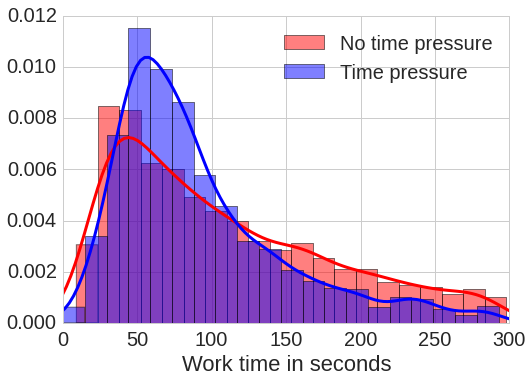
\includegraphics[width=0.4\textwidth]{img/answering_time_distribution}
	\caption{Distribution of answering times for experiments with and without time pressure}
	\label{fig:answering_time_distribution}
\end{figure}

\subsubsection{Answer quality comparison}
\label{section:crowdsourcing:approach:experiments:comparison}

Finally, to compare the quality of the collected answers with automatic system and CQA responses we pooled together the crowdsourced answers, the answers from the winning and other top-10 LiveQA'15 systems, and the original answers crawled from Yahoo! Answers.
We took a sample of 100 questions and repeated the answer rating experiment on this data.
Each answer was judged by 3 different workers (without time pressure), and their scores were averaged.
Figure \ref{figure:crowdsourcing:average_score} displays the plot with average score for answers from different sources.
Quite surprisingly the quality of collected answers turned out be comparable to those of CQA website users.
Average rating of answers produced by the winning TREC LiveQA system is also pretty close to human answers.
Finally, as expected, time pressure had its negative effect on the quality, however it is still significantly better than quality of an average top 10 QA system.

\begin{figure}[h]
	\centering
	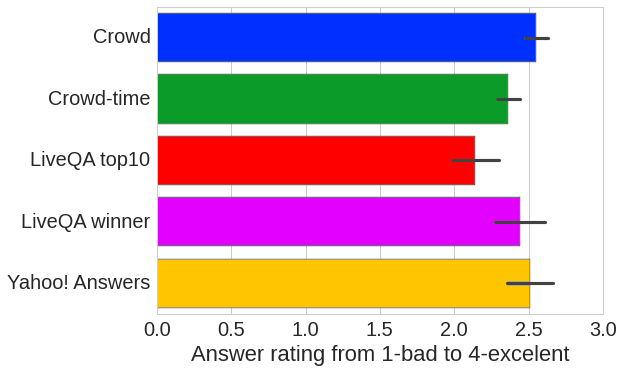
\includegraphics[width=0.4\textwidth]{img/average_score}
	\caption{Average scores of different types of answers to Yahoo! Answers questions}
	\label{figure:crowdsourcing:average_score}
\end{figure}

\begin{figure}[h]
	\centering
	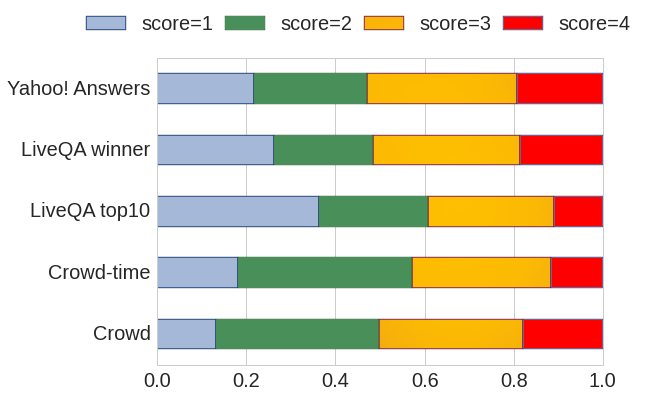
\includegraphics[width=0.4\textwidth]{img/scores_distribution}
	\caption{Distribution of scores for different types of answers to Yahoo! Answers questions}
	\label{figure:crowdsourcing:scores_distribution}
\end{figure}


Analysis of the score distribution (Figure \ref{figure:crowdsourcing:scores_distribution}) sheds some light on the nature of the problems with automatic and human answers. The automatic systems generate non-relevant answers ($score=1$) more often than human, either because the systems fail to retrieve relevant information, or to distinguish between useful and non-useful answer candidates. However, by having a larger information store, e.g., the Web, automated QA systems can often find a perfect answer ($score=4$), while crowd workers tend to give generally useful, but less perfect responses ($score=2,3$).

Our results suggest that the ``crowd'' can quickly give a reasonable answer to most CQA questions. However, some questions require a certain expertise, which a common crowd worker might not possess.
One idea to tackle this challenge is to design a QA information support system, which a worker can use to help them find additional information.
For example, in our experiment, we let workers use web search to find answers, if they were unfamiliar with the topic; more effective search interfaces may be helpful.

The findings of these experiments were used to implement our CRQA system, which stands for Crowd-powered Real-time Question Answering.
CRQA integrates a crowdsourcing module into an automated question answering system within an overall learning-to-rank framework for selecting answers to complex questions.
We report extensive experiments of stress-testing the CRQA system, by participating in the TREC LiveQA 2016 evaluation challenge, which provided us with a realistic evaluation setup.


\subsection{CRQA: Crowd-powered Real-time Automated Question Answering System}
\label{section:crowdsourcing:approach:crqa}

Our CRQA system represents a hybrid system, that includes an automated question answering and crowdsourcing modules.
The high level architecture is presented in Figure~\ref{figure:crowdsourcing:system}.

\begin{figure*}[h!t]
	\centering
	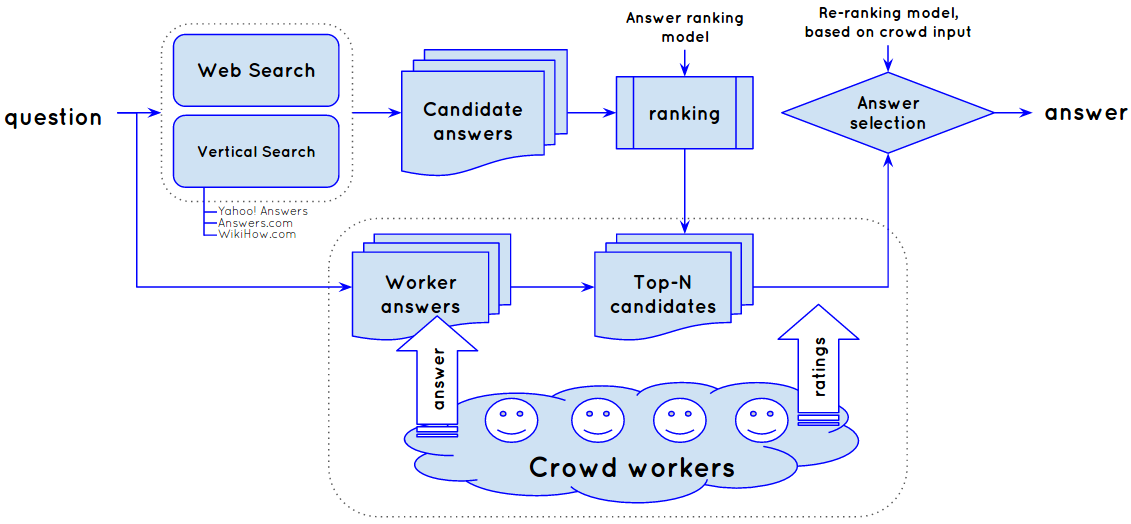
\includegraphics[width=\textwidth]{img/crqa_system}
	\caption{The architecture of our Crowd-powered Real-time Question Answering system, that uses crowdsourcing to augment a list of automatically extracted candidate answers and to rate their quality}
	\label{figure:crowdsourcing:system}
\end{figure*}

The automated part of the CRQA system follows an Information Retrieval (IR) approach to question answering, and generates a set of candidate answer passages from multiple data sources.
After candidates are generated, they are ranked by a trained model, and in the fully automated mode the top candidate could be returned as the answer.
The crowdsourcing module is designed to overcome two of the most common problems of the automated QA approaches: lack of good candidate answers and ranking errors.
More particularly, CRQA asks crowd workers to provide answers to the given questions if they can, and additionally rate the quality of candidate answers, generated by the automated system.
Worker contributions are then used by a trained re-ranking model, that selects the best candidate answers using all the information available.
The next two sections describe the architectures of the automated and crowdsourcing modules of our system.

\subsubsection{Automated question answering module}
\label{section:crowdsourcing:approach:crqa:auto}

When CRQA receives a question, it generates a set of search queries to retrieve a set of relevant documents and extract candidate answer passages.
Search queries are generated using the following strategies:
\begin{itemize}
\item Question title, which most often captures the gist of the question
\item Two longest question sentences (detected by the presence of the question word at the beginning or question mark at the end of a sentence) from the title and body of the question. In some cases the real user question is hidden inside the body, while the title just provides the overall topic of the question.
\item Concatenation of the question word, verbs and top-5 terms from the question title by Inverse Document Frequency\footnote{IDF of terms are estimated using Google N-gram corpus: https://catalog.ldc.upenn.edu/LDC2006T13}. This strategy targets over-specific questions, which often retrieve few if any search results.
\end{itemize}

To retrieve a set of potentially relevant documents and extract candidate answer passages, CRQA relies on multiple different generic and CQA document collections.
Previous research \cite{Shtok:2012:LPA:2187836.2187939} has shown that many of the user information needs are repeated, and reusing answers to previously posted similar questions is an effective strategy for answering new questions.
Therefore, CRQA uses multiple different CQA data sources, which potentially contain a diverse set of questions.
However, quite often it is hard to find a similar question in an archive, and many of the information needs are unique.
Therefore, we include a web search component, that can retrieve regular web documents, from which our system can extract candidate answers.
More specifically, CRQA queries the web using Bing Web Search API\footnote{https://datamarket.azure.com/dataset/bing/searchweb}, Yahoo! Answers, Answers.com and WikiHow.com using their respective search interfaces.
For each query we retrieve top-10 relevant documents and question-answer pairs from CQA archives.
As candidate answers CRQA extracts answers to the questions retrieved from CQA results and paragraphs of text from the main content of regular web documents, as detected by a method based on \cite{Kohlschutter_2010}.
Quite often, it is hard to estimate the quality of a candidate answers from its text only.
The task becomes much easier if a system has access to additional data, \eg for the candidates generated from the CQA archives, it is useful to know the text of the original question the candidate answers.
For candidates, generated from regular web pages, it is useful to know the topic of the page (\eg from its title), additionally the context of the candidate, such as text that immediately precedes it in the document was shown to provide a useful information for QA.
Therefore, besides the text of a candidate answer, we keep some potentially useful metadata, \eg for QnA candidates we include text and category of the retrieved question, and web page title and text block preceding the answer passage in the document for web-search based candidates.
For convenience, we will call the title of a retrieved question or web page \textit{``the answer topic''}, and the body of the retrieved question or the preceding text block the \textit{``the answer context''}.

Next, for each candidate answer we compute a set of features, described in Table \ref{table:crowdsourcing:crqa:features}.

\begin{table}[ht]
\centering
\begin{tabular}{| p{12cm} |}
\hline
\textbf{Answer statistics} \\
\hline
--- Length in chars, words and sentences \\
--- Average number of words per sentence \\
--- Fraction of non-alphanumeric characters  \\
--- Number of question marks \\
--- Number of verbs  \\
\hline
\textbf{Answer source} \\
\hline
--- Binary feature for each of the search verticals: Web, Yahoo! Answers, Answers.com, WikiHow.com \\
\hline
\textbf{N-gram matches}\\
\hline
--- Cosine similarities using uni-, bi- and tri-gram representations of the question title and/or body, and answer text, topic or context\\
--- The lengths of longest spans of matched terms between question title and/or body, and answer text, topic or context\\
\hline
\textbf{Information Retrieval score}\\
\hline
--- BM25 scores between question title and/or body, and answer text, topic or context\\ 
\hline
\end{tabular}
\caption{The list of candidate answer ranking features used by the automated module of our CRQA system}
\label{table:crowdsourcing:crqa:features}
\end{table}

The final stage of the module is answer ranking, where a trained LambdaMART \cite{burges2010ranknet} model sorts the candidates by their predicted quality.
This model was trained using the RankLib library\footnote{https://sourceforge.net/p/lemur/wiki/RankLib/} on the data from last year TREC LiveQA task\footnote{https://sites.google.com/site/trecliveqa2016/liveqa-qrels-2015}, which includes 1087 questions with answers provided by the participants, each of which was rated on a scale from 1(bad) to 4(excellent) by professional NIST assessors.
In a fully automated setup the top candidate could be returned as the final answer to the question, but in this work we explore if we can further improve the performance of the system using crowdsourcing.

\subsubsection{Crowdsourcing module}
\label{section:crowdsourcing:approach:crqa:crowdmodule}

As we mentioned before, two of the main problems with the fully automated system responses are lack of good candidates and problems with ranking, therefore, we decided to explore if crowdsourcing can be helpful to overcome these challenges in near real-time scenario.
Instead of returning the final answer, the system sends the question and top-7 ranked candidates to the crowd workers and waits for the responses.
We chose to give 7 answers based on the average number of rated answers in our preliminary studies.
Since systems had only 60 seconds to answer each question, we start a timer when a question arrives, and the system waits to receive all worker contributions until the timer reaches 50 seconds to leave the system some time to generate the final answer and minimize the chances of going above the time limit.
CRQA asks workers to write their own answers to questions if possible, which should provide additional candidates in case there are no good automatically generated ones.
Additionally, systems expects workers to rate the quality of top-7 ranked candidates, which should help to fix the ranking problems and select a better final answer.
Figure~\ref{figure:crowdsourcing:crowd_ui} presents the user interface of our crowdsourcing module.

\begin{figure*}[h!t]
	\centering
	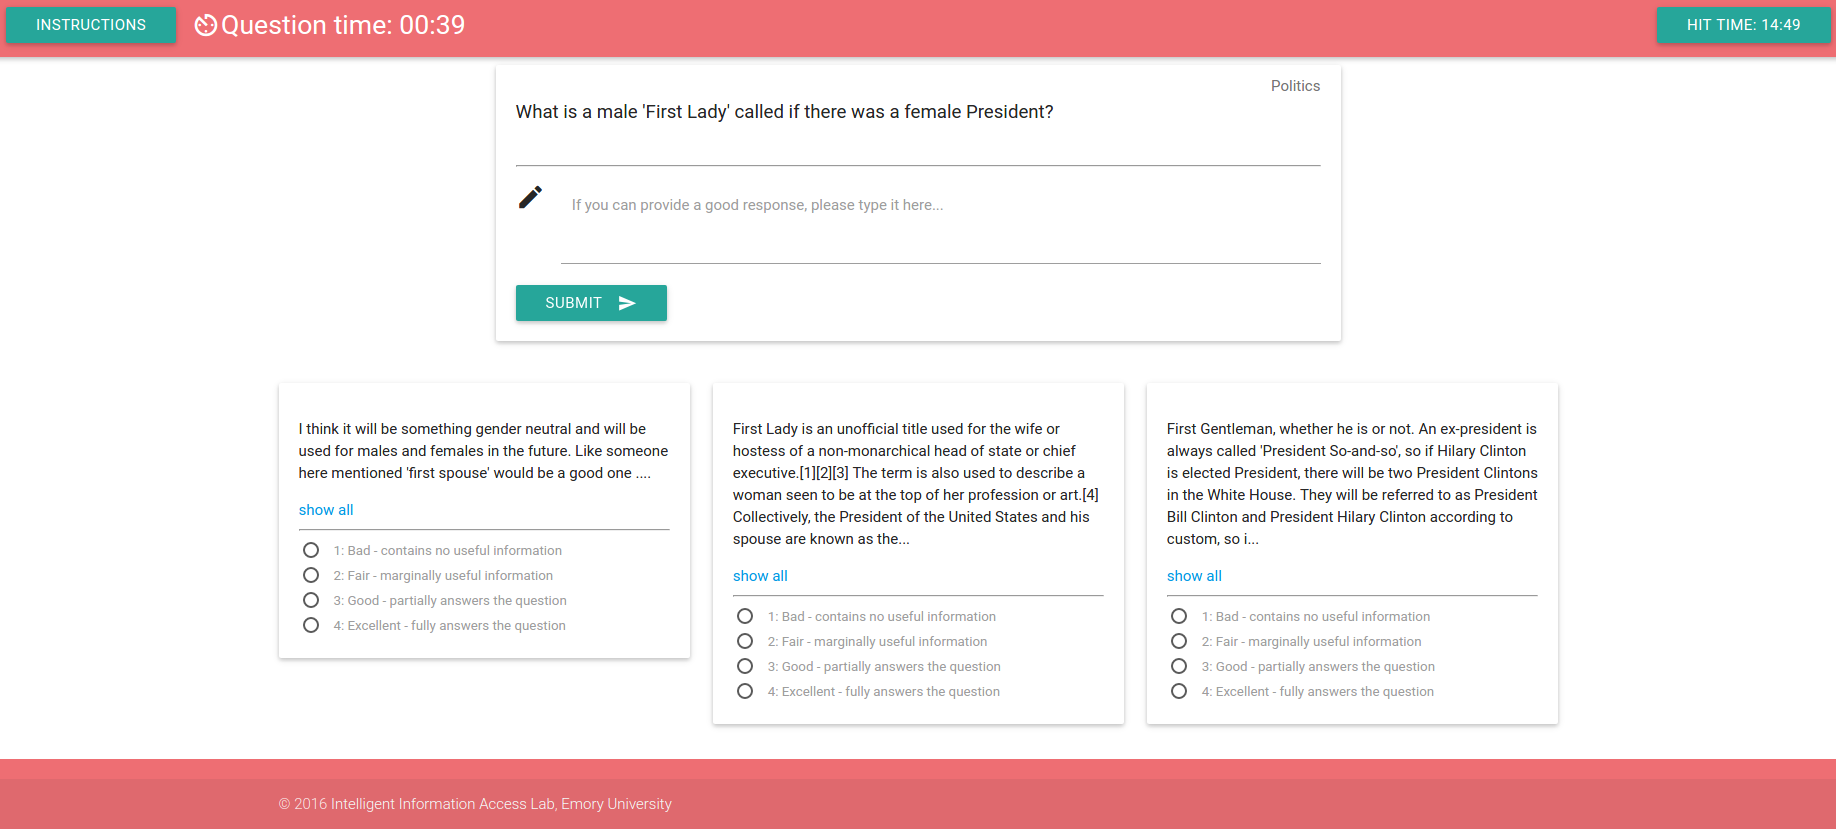
\includegraphics[width=\textwidth]{img/crqa_crowd_ui}
	\caption{User Interface for workers in our Crowd-Powered Question Answering system}
	\label{figure:crowdsourcing:crowd_ui}
\end{figure*}

The overall algorithm for obtaining crowd input for real-time question answering is the following:
\begin{enumerate}
\item When a system receives a question, it is posted to the workers, who will have 50 seconds to provide their input
\item Workers are asked to write an answer if they can provide one (it is optional)
\item Otherwise they are waiting for the answer candidates to arrive
\item When a system is done with generating and ranking candidates it posts top-7 scoring answers to the workers for the rating (which usually leaves $\sim$ 35 seconds for rating)
\item Workers receive a list of answers\footnote{Answers submitted by workers are also sent for ratings to all workers except the author} and rate them until the timer runs off. Each answer is rated on a scale from 1 to 4, using the official TREC LiveQA rating scale:
	\begin{itemize}
    \item 1 --- Bad: contains no useful information
    \item 2 --- Fair: marginally useful information
    \item 3 --- Good: partially answers the question
    \item 4 --- Excellent: fully answers the question
    \end{itemize}
\item The interface displays 3 answers at a time, when an answer gets rated, it disappears and its place is taken by another answer from the pool. The interface displays only the first 300 characters of the answer, which was experimentally shown to be enough on average to make a good judgment.
Full answer can be revealed upon clicking the ``show all'' link.
\item When the timer runs off, the question and all the answers disappear, and workers wait for the next question
\end{enumerate}

% Not sure we need a title, as this subsection already describes the crowdsourcing module.
% \noindent\textbf{QARC system implementation: Crowd module}:
To hire the workers we used Amazon Mechanical Turk platform\footnote{http://mturk.com}.
Since the challenge was to run the system ``live'' over the period of 24 hours, we adapted the ``retainer'' model to our question-answering task, inspired by the success of this model reported in previous work \cite{bernstein2011crowds,bigham2010vizwiz}.
Specifically, to obtain an even distribution of workers over the 24-hour period of the TREC LiveQA shared task, we posted 10 tasks every 15 minutes, and they expired after the next set of tasks became available.
Since not all assignments were accepted by some worker right away, the number of workers for each question varied and could be greater than 10.
When a worker first gets to our crowdsourcing interface, she is shown task instructions (Table \ref{table:crowdsourcing:crqa:crowd_instructions}) and asked to wait for the questions to arrive.
The workers were paid \$1.00 for the whole 15 minutes task, no matter how many questions they got\footnote{In TREC LiveQA task questions are sent to the systems one by one, therefore there is no concurrency, however the delays between the questions are possible}.

\begin{table}[ht]
\centering
\begin{tabular}{| p{15cm} |}
\hline
\textbf{Instructions} \\
\hline
1. This HIT will last exactly 15 minutes\\
2. Your HIT will only be submitted after these 15 minutes\\
3. In this period of time you will receive some questions, that came from real users on the Internet\\
4. Each question has a time limit after which it will disappear and you will need to want for the next one\\
5. If you know the answer to the question, please type it in the corresponding box\\
6. At some point several candidate answers will appear at the bottom of the page\\
7. Please rate them on a scale from 1 (bad) to 4 (excellent)\\
8. Do not close the browser or reload the page as this will reset your assignment.\\
\hline
\end{tabular}
\caption{Crowdsourcing task instructions, displayed to the user when she first gets to the task}
\label{table:crowdsourcing:crqa:crowd_instructions}
\end{table}

\textbf{Answer re-ranking and selection}.
The last stage in CRQA is answer re-ranking, which aggregates all the information received from the crowdsourcing and produces the final answer to the question.
The input of the re-ranking module is a set of candidate answers with quality ratings provided by the crowd workers.
Candidates can include the answers posted by the workers, which might also be rated, if workers had enough time to do that.
To re-rank the answers we trained a gradient boosting regression trees (GBRT) model \cite{friedman2002stochastic}.
To build this model we used a training set of questions with answers generated by our system.
The quality of each answer was manually assessed using the official LiveQA scale from 1 (bad) to 4 (excellent).
The features, used for answer re-ranking are listed in Table~\ref{table:crowdsourcing:crqa:reranking_features}.

\begin{table}[ht]
\centering
\begin{tabular}{| p{15cm} |}
\hline
\textbf{Answer-based} \\
\hline
--- The length of the answer \\
--- Source of the answer (Crowd, Web, Yahoo! Answers, Answers.com or WikiHow.com)\\
--- Original rank of the candidate answer or -1 for answers provided by the crowd workers\\
\hline
\textbf{Worker ratings} \\
\hline
--- Number of ratings provided\\
--- Minimum, maximum, median and average ratings\\
\hline
\end{tabular}
\caption{The list of features used for answer re-ranking based on crowdsourcing input}
\label{table:crowdsourcing:crqa:reranking_features}
\end{table}

CRQA sorts the candidates by the quality score predicted by the model, as returns the top candidate as the final answer.


\subsubsection{Experiments}
\label{section:crowdsourcing:approach:crqa:experiments}


We now describe the experimental setup used to evaluate the performance of CRQA and other methods for near real-time question answering.

The experimental evaluation of our CRQA system was done on the official run of TREC LiveQA shared task, which happened on May 31, 2016.
All participating systems were running for 24 hours and received questions sampled from the live (real-time) stream of questions, posted by real users to Yahoo! Answers platform.
In total, each system received 1,088 questions, and system responses were recorded by the organizers.

\begin{table}[ht]
\centering
\begin{tabular}{| p{14cm} | c | }
\hline
Name & Value \\
\hline
Number of questions received & 1088 \\
Number of completed assignments (15 mins each) & 889 \\
Average number of questions per assignment & 11.44 \\
Total cost per question & \$0.81 \\
Average number of answers provided by workers & 1.25 \\
Average number of ratings per answer & 6.25 \\
\hline
\end{tabular}
\caption{Aggregate statistics of crowdsourcing tasks}
\label{table:crowdsourcing:crqa:task_stats}
\end{table}

Overall statistics are provided in Table~\ref{table:crowdsourcing:crqa:task_stats}.
As we can see, on average workers were able to provide at least one answer for each question, and each of the provided answers got 6 ratings.
Since the interface could show only 3 answers at a time, answers had different chances of being rated.
To investigate the effect of the order of the candidates posted for ratings on the quality of the final answer, in CRQA for each worker and each question we randomly selected one of the strategies: ordering answer candidates by their model rank or random shuffling of the candidates.
The system variant with shuffled candidates for rating was expected to obtain more diverse and comprehensive set of ratings, as we will investigate in the Analysis section.

The official results of the shared task will be available in November 2016 during the TREC conference\footnote{http://trec.nist.gov/}.
Meanwhile, we used traditional (batch-mode) crowdsourcing to obtain the quality labels for all answer candidates that were given to the workers during the task, as well as the answers provided by the workers.
In addition, on June 2, two days after the TREC LiveQA challenge has completed, we crawled the current answers provided by the community for the questions, used for the task.
All the answers for each question were randomly shuffled and rated on a scale from 1 (bad) to 4 (excellent) by workers hired on Amazon Mechanical Turk.
As we have shown in the previous section, crowdsourced labels correlates well with the official ratings, provided by the professional NIST assessors.
Each answer was labeled by 3 different workers, and we averaged the scores to get the final quality labels for the candidates.

We compared CRQA system against several baselines:
\begin{itemize}
\item \textit{Automated QA}: automated QA system described in Section~\ref{section:crowdsourcing:approach:crqa:auto}.
\item \textit{CRQA}: Automated QA system with Crowdsourcing, described in Section~\ref{section:crowdsourcing:approach:crqa:crowdmodule}
\item \textit{Re-ranking by score}: a simplified version of CRQA re-ranking model, which select the answer with the highest average ratings, provided by the crowd workers.
\item \textit{Yahoo Answers}: traditional, non-real-time community question answering site (Yahoo Answers), from which the challenge question originated. The answers were collected two days after the challenge, thus allowing the Yahoo Answers community extra two days to collect the answers through traditional (community-based) crowdsourcing.
\end{itemize}

To evaluate the methods we used the metrics proposed by the organizers of the LiveQA task:
\begin{itemize}
\item \textbf{avg-score}: average score over all questions
\item \textbf{avg-prec}: average score over all answered questions
\item \textbf{s@i+}: the fraction of answers with score i or greater (i=2..4)
\item \textbf{p@i+}: the number of answers with score i or greater (i=2..4) divided by the number of answered questions\footnote{Since for each answer we averaged 3 ratings by different workers, the number of answers with the average score of 4 is low}
\end{itemize}

\begin{table*}[ht]
\centering
\begin{tabular}{| p{4.2cm} | c | c | c | c | c | c | c | c |}
\hline
Method & avg-score & avg-prec & s@2+ & s@3+ & s@4+ & p@2+ & p@3+ & p@4+ \\
\hline
Automated QA & 2.321 & 2.357 & 0.697 & 0.297 & 0.026 & 0.708 & 0.302 & 0.026 \\
Re-ranking by score & 2.416 & 2.421 & 0.745 & 0.319 & 0.031 & 0.747 & 0.320 & 0.031 \\
Yahoo! Answers & 2.229 & 2.503 & 0.656 & 0.375 & \textbf{0.045} & 0.737 & \textbf{0.421} & \textbf{0.050} \\
CRQA & \textbf{2.550} & \textbf{2.556} & \textbf{0.799} & \textbf{0.402} & 0.034 & \textbf{0.800} & 0.402 & 0.034 \\
\hspace{5mm}worker ratings only & 2.432 & 2.470 & 0.750 & 0.348 & 0.030 & 0.762 & 0.354 & 0.031 \\
\hspace{5mm}worker answers only & 2.459 & 2.463 & 0.759 & 0.354 & 0.029 & 0.760 & 0.355 & 0.029 \\
\hline
\end{tabular}
\caption{Evaluation of the baselines and system answers quality based on the ratings of answers obtained via crowdsourcing. The scores are averaged over 100 different 50:50 splits of 1088 questions into the training and test set. The differences between average score and precision of CRQA and the original ranking are significant at p-value $<$ 0.01}
\label{table:crowdsourcing:crqa:performance}
\end{table*}

Table~\ref{table:crowdsourcing:crqa:performance} summarizes the performance of the baselines and our system.
As we can see, the average score and precision of answers generated by CRQA system is higher than the baseline ranking and even community answers on the Yahoo! Answers platform.
However, Yahoo! Answers community answers have higher percentage of \textit{``4 (excellent)''} scores.
Figure \ref{figure:crowdsourcing:crqa:score_histogram} shows the distribution of scores for the original system ranking, our crowdsourcing system and Yahoo! Answers.
Two peaks on the distribution of scores from Yahoo! Answers community suggest, that there are essentially two kinds of responses: non-useful (\eg spam) or excellent that fully answers the question.
In addition, around 20\% of the questions did not get any answer from the community.
Automatically generated answers, on the contrary, are rarely empty, but on average provide only marginally relevant information, which often does not answer the questions, and therefore rated \textit{``2 (fair)''}.
The introduction of the crowdsourcing module allowed CRQA to cover a couple of percent of the questions, for which the automated system was not able to generate any candidates, as well as select better candidates when it was possible using crowd ratings.

\begin{figure}[h]
	\centering
	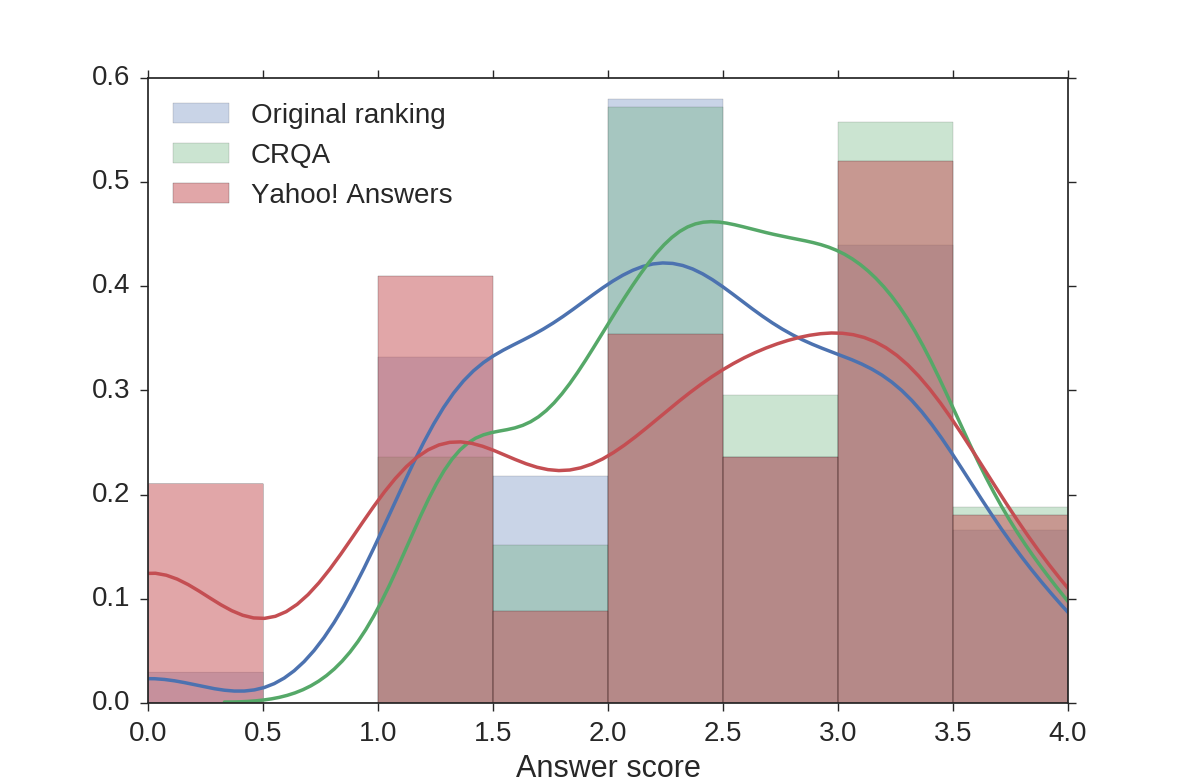
\includegraphics[width=0.5\textwidth]{img/crqa_score_hist}
	\caption{Histogram and kernel density estimation of answer scores for original candidate ranking, CPQA model re-ranking and Yahoo! Answers answers}
	\label{figure:crowdsourcing:crqa:score_histogram}
\end{figure}

Therefore, we can conclude, that crowdsourcing can effectively help automated QA system to improve the performance of question answering, by providing worker generated answers and rating existing candidates.

\subsubsection{Analysis}
\label{section:crowdsourcing:approach:crqa:analysis}

In this section we will analyze some of the results of our experiments and discuss their implications.

\textbf{Worker answers vs ratings}.
First, let's look at the contribution of additional answers and answer ratings provided by the workers.
These two types of contributions are complimentary to each other and attempts to solve different problems.
Table \ref{table:crowdsourcing:crqa:performance} shows the performance of our question answering system using each of these types of feedback independently.
The results demonstrate that both answers and ratings have positive effect on the performance.
Even with limited time, workers were able to reliably rate candidate answers, which helped the system to select a better final answer and improve the model precision.
However, this method does not help the system in cases, when it was not able to generate a good candidate in the first place, therefore using ratings only has lower average answer score than using worker generated answers.
By asking the crowd to provide a response if they can answer the question, CRQA covers this gap, which is important as in a real scenario even a fair answer would probably be better for the user than no answer at all.
Of course, given limited time and the fact that a random worker might not possess an expertise required to answer the question, such answers do not always perfectly answer the question.
Table \ref{table:crowdsourcing:crqa:answer_examples} gives some examples of worker generated answers with low and high quality scores.

To summarize, ratings of answer candidates and worker generated answers both have similar positive effect on the performance of our question answering system.
What is more important, the contributions are independent and therefore it is beneficial to use both of them in the final system.

\begin{table*}[ht]
\centering
\begin{tabular}{| p{10.5cm} | p{5cm} | c |}
\hline
Question & Answer & Score \\
\hline
 Is Gotu Kola a good herb for mental health? How long does it take to work?? & yes & 1.66\\
 \hline
Can I write any number on line number 5 of a W2?  would like to set up my W2 were I get the most out of my paycheck and not have to pay taxes at the end of the year... & W2 & 1.33\\
 \hline
I need help with my mum? Something traumatic happened to me about 4 years ago i randomly asked my mother why when I lived with you in your home country a man that was our neighbour used to call me his daughter and the younger kids that lived there called me there cousins and one boy called me his sister? & yes & 1.0\\
\hline
\hline
 Is it bad not wanting to visit your family? & It is nt bad. Just be honest with them. They may be upset but they should understand & 3.0 \\
 \hline
Any health concerns with whey protein? So I workout 3-5 days a week and i drink a whey protein isolate after each workout. Since I workout almost everyday, is it ok for me to just drink a shake everyday?.. & As long as you use it as directed, there should not be any major problems.  You may want to consult your doctor just in case, but I would not be too concerned. & 3.0\\
\hline
Foot pain unable to walk? Hi so today woke with some pain, I am able to put weight on my heel with no problem or pain.  But  the area between my heel and toes hurts really bad when I try to go with the motion of taking a step. Its not swollen and I do not remember hurting it at all & Possible gout in your foot, also possible you may have strained it during the previous day. & 3.0\\
\hline
What is a good remedy/medicine for stomach aches? Specifically ones caused by stress or anxiety? & Chamomile tea should help & 3.66\\
\hline
\end{tabular}
\caption{Examples of answers provided by the crowd workers and their average quality scores}
\label{table:crowdsourcing:crqa:answer_examples}
\end{table*}

\textbf{Selection of answer candidate for rating}.
Predicting the quality of answers and ranking them to select the best is one of the main challenges in automated question answering \cite{surdeanu2011learning}.
External feedback, such as noisy answer ratings, obtained from the crowd workers, provide valuable information, which, as our results demonstrate, can help a QA system to better re-rank the answers.
However, the capacity of crowdsourcing for answer ratings are obviously limited, as systems often are dealing with hundreds and thousands of answer candidates for a given question.
In this work, we made a choice to rate only top-7 answers according the automated system ranking.
This decision was made based on the average number of ratings workers could provide in the allotted time\footnote{The answers were posted for rating automatically after an automated system was done with candidate generation and ranking. On average users had $\sim$ 35 seconds to provide the ratings.}.
However, the order in which the answers are shown can also have a strong effect on the system performance, because the answers are typically rated one by one in the order they are displayed on the screen.
Our system included two strategies for answer ordering: random or according to their ranking score.
The former strategy provides a uniform coverage for all the answers selected for rating, while the later puts more emphasis on the currently top scoring candidates.
We randomly selected one of the strategies for each user and question.
To analyze the performance of each of the strategies we compute the average score of answers, generated using the corresponding ratings.
The average score for answers generating when candidates are shuffled is 2.508, and it is 2.539 when the candidates are sorted according to their model ranking score.
This suggests, that it is beneficial to allocate more of the workers attention on the top scoring candidate answers.

\textbf{Cost analysis}.
The results of our experiments clearly demonstrated that crowdsourcing can improve the performance of near real-time question answering system.
The next reasonable question is what is the price of this improvement.
In our study we paid workers \$1.00 per single 15 minutes task, and each 15 minutes we had 10 assignments, which translates to \$15.00 per 15 minutes.
Overall, our experiment cost \$0.88 per question, and in this section we will discuss some ideas to reduce this cost.

First, we will study the effect of the number of workers on the performance of our CRQA system.
For this experiment we randomly sampled certain percentage of workers and removed all contributions (answers and ratings) of others.
Figure \ref{figure:crqa:nworkers_vs_quality} plots the dependency of the performance of our QA system on the number of workers.

\begin{figure*}[h!t]
  \begin{subfigure}[t]{0.5\textwidth}
	\centering
	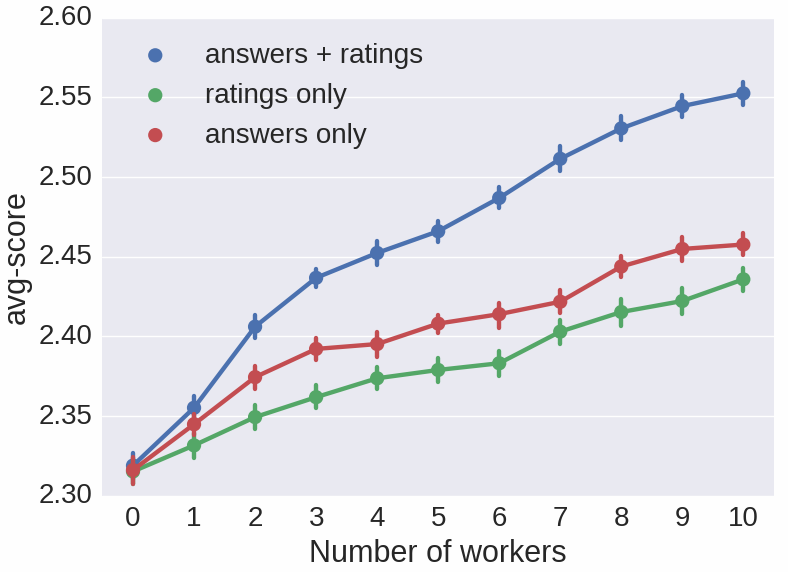
\includegraphics[width=\textwidth]{img/crqa_nworkers_vs_accuracy}
	\caption{avg-score: Average score per question}
	\label{figure:crqa:nworkers_vs_accuracy}
  \end{subfigure}
  \begin{subfigure}[t]{0.5\textwidth}
	\centering
	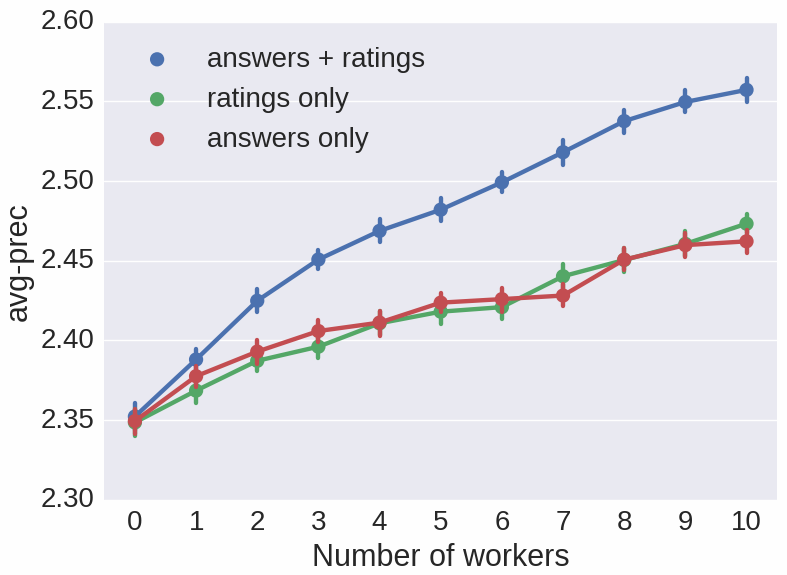
\includegraphics[width=\textwidth]{img/crqa_nworkers_vs_precision}
	\caption{avg-prec: Average score per answer (ignoring non-answered questions)}
	\label{figure:crqa:nworkers_vs_precision}
  \end{subfigure}
	\caption{Plot showing how the quality of the final answer depends on the number of workers per question}
	\label{figure:crqa:nworkers_vs_quality}
\end{figure*}

Obviously more workers mean more reliable answer ratings and more answer candidates, which improves the performance of the question answering system.
However, we can observe diminishing returns, as the cost per extra gain in performance metrics decreases as the number of workers grow.
Half of the overall performance improvement could be achieved with only 3 workers per question, which would save 70\% of the costs.

An alternative cost-reduction strategy is selective triggering of crowdsourcing, which would only ask for workers feedback for some of the questions.
Such a strategy would be necessary to scale a crowd-powered question answering system to a higher volume of questions.
There are multiple different approaches for such selective crowdsourcing: \eg a system can only ask for crowd contributions if it did not generate enough candidate answers or the predicted quality of the top scoring candidates is low \cite{carmel2010estimating,he2006query}.
We leave this questions for the future work, as here we focused on the scenario, proposed by the organizers of the TREC LiveQA shared tasks, where questions arrive one by one and it is possible to utilize crowd input for every questions.

To summarize, in the explored real-time QA scenario it is possible to reduce the costs of crowdsourcing by reducing the number of workers, although with some performance losses.
Our analysis suggests that paying 30\% of the original cost would give 50\% of the performance improvement.

\subsection{Summary}

In this section we presented CRQA, the first, as far as we know, real-time question answering system that integrated crowd work within an automated question answering system.
Specifically, we explore different methods of obtaining input from the crowd, and use a machine-learned answer re-ranking model that incorporates the crowd input as features to select the final system answer to return to the user. 

We report a large-scale experiment in which over a thousand real user questions were submitted to the CRQA system in real-time, as part of the LiveQA challenge.
CRQA was able to successfully answer these questions in under 1 minute, with over 80\% of the answers subsequently rated to be fair or better.
Importantly, CRQA significantly improved question quality and coverage compared to the starting automated-only system, and, surprisingly, was able to return better answers on average compared to the traditional CQA system with millions of users (Yahoo! Answers) with answers collected more than \textit{two days} after the original posting time.

The described CRQA implementation is a promising step towards efficient and close integration of crowd work and automated analysis for real-time question answering.
It raises many promising issues and opens directions for future work, such as selective crowdsourcing for only the questions deemed ``difficult'' for the automated system; more efficient online learning for obtaining ratings from the crowd and integrating them into the ranking model; and investigating additional features and sources of evidence for improving the joint ranking of the system and crowd input.
This section describes a flexible and powerful framework for combining the powers of crowdsourcing with automated question answering techniques, for building the next generation of real-time question answering systems.

\section{Proposed Directions for Future Research}
\label{section:crowdsourcing:proposal}

The results described above demonstrate how effective can crowdsourcing be for real-time question answering.
However, it can also be quite expensive, which is one of the most critical problems for scalability of hybrid system.
Such a system needs to have a good strategy to deal with increasing volume and velocity of the input data, \ie user questions.
CRQA system, developed to participate in TREC LiveQA cost us \$0.81 per question, which is quite expensive, and according to our analysis in Section~\ref{section:crowdsourcing:approach:crqa:analysis} it is possible to get half of the performance gain for 30\% of the costs by hiring less workers.
However, in general such a strategy is not agile enough, as some questions might be very easy and system do not actually need any worker input, while some others are very hard and would benefit from more human feedback.
In addition, in different situations our hybrid system might need different types of feedback, \eg for some questions some help with answer ranking is more important than additional candidates, and sometimes the opposite.

The research proposed below targets the problem of designing an optimal crowdsourcing plan, \ie allocation of crowdsourcing resources across different tasks.
The first step towards this goal is to develop a model for selective crowdsourcing, \ie identification of cases when an automated system would benefit from crowdsourcing the most and when it might be redundant.
Next, if a system decides to request feedback from crowdsourcing, we need to decide how much resources to allocate (number of workers and time) and where to target it (what kind of feedback to request from how many users).

% \todo{We also had an idea to utilize feedback more efficiently. The system might rerank all candidates based on feedback, or it can even request more candidates using worker feedback}
% \todo{User expertise and question routing, a lot of previous research. Except based on feedback a user provided, estimate her trustworthiness, expertese and whether she better rates or answers questions}

\subsection{Method}
\label{section:crowdsourcing:method}

First, we need to formulate the conditions and objectives of the problem we are trying to solve, \ie resource and quality conditions, etc.
An important problem to focus on in the future research is optimizing the quality of hybrid question answering under the fixed crowdsourcing budget.

A possible approach on the problem is to stick with the real-time scenario, proposed in TREC LiveQA challenge, and set the maximum response time to 1 minute after the question is posted.
In such scenario, for the selective crowdsourcing problem one can train a machine learning model to predict the expected performance of the answer, given all the current candidates.
This problem is very similar to search query performance prediction~\cite{carmel2010estimating,he2006query,zhou2007query}, and therefore we can adapt the ideas developed in this line of research.
More specifically, a machine learning model (\eg random forest or gradient boosted regression trees) can be trained to predict the expected relevance score of the answer a system is about to return, given the following set of features:
\begin{itemize}
\item single answer features: answer length, information retrieval score given the question text and other features used for answer ranking
\item results list features: syntactic and semantic similarity of the top answer to other retrieved candidates
\item corpus dependent features: query clarity score~\cite{cronen2002predicting}, which measures the coherence of the retrieved results (answer candidates) with respect to the whole corpus
\end{itemize}

In the simplest case, the score, returned by this model, can be thresholded to determine if the answers is expected to be good and no crowd feedback is needed, or if the system would benefit from worker contributions.
Alternatively, it is possible to experiment with adaptive thresholding, which can be implemented by putting all the questions into a single priority queue, based on their expected quality from lowest to highest.
The workers will be assigned to the tasks from the top of the queue, \ie starting from the lowest expected performance.
Decision on how many workers assign to which tasks depends on many factors, such as total number of workers available, number and expected performance of other questions expecting crowdsourcing feedback in the queue.
Therefore, to design a resource allocation strategy I will train another machine learning model, that will predict how much workers to assign to each question, given the total number of workers and information about the other questions waiting in the queue, \ie expected performances of 2nd, 3rd, ... questions in the queue, waiting time for the other questions in the queue, \etc.
Such a model will allow a system to adapt not only to varying number of workers available, but also to changing velocity of the arriving questions.

Finally, another important aspect of crowdsourcing for real-time question answering is how much time do we need to give to workers in order to receive enough feedback.
To answer it, we can analyze the data we already collected and determine the dependency of performance gain vs time workers spend on the task, which can be done by filtering out feedback items received after certain time threshold.

\subsection{Experimentation}
\label{section:crowdsourcing:experiments}

To train the models and conduct the analysis of the work proposed in the previous section we can use the crowdsourcing data we already collected during TREC LiveQA 2016.
The dataset includes 1088 questions, top 7 automatically and worker generated answers, each of which was judged on a scale from 1 - 4 based on its relevance to the question.
This setup allows us to apply different reranking and filtering strategies and estimate the final quality of the answer our hybrid system would return.

To train the selective crowdsourcing model the dataset can be split into training, development and test sets, and the training portion can be used to build a regression model to predict the relevance of top answer given the question and other candidates, represented by a set of features described above.
To test this model, we can apply it on a test set and compute Pearson and rank correlation coefficients.
In addition, by varying the threshold we can save certain percentage of crowdsourcing resources by discarding the corresponding feedback data and draw the performance vs crowdsourcing cost plot.

Finally, to model a real scenario of questions arriving non-uniformly in time, we can modify the dataset and set question posting times based on some random process, \eg Poisson point process.
To simulate various situations, I will generate three different datasets with different parameters to test the behavior in low, moderate and high load situations.
Each dataset will be split by time into training and test, and I will train the resource allocation model (predicting how many workers to allocate to the task) on the training set and use it on training set.
The output of the model will be used to subsample the feedback of the users we already have, \eg if the model suggests to use 4 workers, we can sample them from a total pool of 10 workers we already had for this task.
Unfortunately, this experiment does not allow us to go beyond 10 workers per question, but this scenario is quite expensive anyway, therefore it seems more reasonable to explore only plans where we do not need to go beyond 10 workers.
In addition, in the original experiment there was no need to share workers between tasks, as all of the tasks arrived sequentially, while in real scenario we will have more than one question requiring worker feedback.

\section{Summary}
\label{section:crowdsourcing:summary}

This section described my prior research and proposed some additional work in developing a crowdsourcing module for real-time question answering.
I developed a crowd-powered automated question answering system, called CRQA, that participated in TREC LiveQA 2016 shared task and by preliminary results significantly improved the performance compared to fully automated scenario.
Additional research I proposed targets mostly the scalability of the system, \ie reducing total costs by applying crowdsourcing selectively to questions that would benefit from it the most and allocating the number of workers according to the total available resources and the volume of the incoming questions.
This work will be included into my thesis if time permits.

The next section will look into another important aspect of question answering, namely interactions with the user.
Despite our best effort to cater to the user information needs, they may be expressed in an ambiguous way or miss some important details, which makes it simply impossible to answer.
In other cases, complex informational tasks may be reduced a number of easier questions, which a system can solve automatically.
To handle all these situations we need to study and improve the ways a question answering system communicates with the user.


% chap6_users.tex
%

\mychapter{User Interactions with Question Answering Systems}
\label{chapter:users}

\noindent

\section{Problem}
\label{section:users:problem}

Most of the research has considered question answering as a one side communication process: a user issues a question and a computer system provides an answer.
Thus, the only input a system receives is the text of the question and the only output is the text of the answer.
This setup is quite limited, because it doesn't provide any means for the user to affect the behavior of a question answering system except by issuing new questions.
Similarly, it doesn't allow QA systems to request any additional information from the user.
However, with the growth of mobile personal assistants and conversational agents the popularity of dialog-based interface increases, which opens up new opportunities for question answering.

TREC complex interactive question answering (ciQA) track, which were run in 2006 and 2007, was designed specifically to motivate research in this area.
In this task participant system could request some input from assessors before submitting the final answer.
However, the setup of the task wasn't exactly based on a dialog between systems and their users.
The most typical approach to the task was to give assessors a set of sentences or passages to judge as relevant/irrelevant and use this feedback to improve the quality of the final answer.
Such scenario is quite problematic to implement in todays personal assistants and chat bots, as they require relatively significant effort and time from users.

In my thesis I'm going to focus on improving the user success solving complex informational tasks in a question answering dialog scenario.
Section~\ref{section:users:approach} describes my prior research on assisting users by providing strategic search hints, designed to help split a complex task into smaller ones that an automatic system will likely handle much better.
And section~\ref{section:users:proposal} proposes additional research to incorporate user feedback into a question answering system in a chat bot scenario.

\section{Approach}
\label{section:users:approach}

%-=-=-=-=-=-=-Search hints begin-=-=-=-=-=-

\subsection{Search Hints for Complex Informational Tasks}
\label{section:users:hints}

Search engines are ubiquitous, and millions of people of varying experience use them on daily basis.
Unfortunately, not all searches are successful.
Bilal and Kirby \cite{Bilal:2002:DSI:637512.637516} reported that about half of the participants of their user study felt frustration when searching.
Xie and Cool \cite{xie2009understanding} demonstrated that most of the time users have problems with formulating and refining search queries.
Besides good retrieval performance, a successful search requires users to possess certain skills.
Search skills can be trained, e.g. Google offers a course\footnote{http://www.powersearchingwithgoogle.com} on improving search efficiency.
Although very useful, such courses are time consuming and detached from real search problems of these particular users.
Displaying search hints is another technique that has both learning effect, and offers immediate assistance to the user in solving her current search task.
Moraveji et al. \cite{Moraveji:2011:MIU:2009916.2009966} demonstrated that hints, suggesting certain search engine functionality, help people find answers more quickly, and the effect is retained after a week without hints.

In this section I explore {\em strategic} search hints, that are designed to guide a user in solving her search problem.
More specifically, we chose the divide-and-conquer strategy, \ie splitting an original difficult question into smaller problems, searching answers to the subtasks and combining them together.
Two sets of strategic hints were manually designed: {\em generic} hints describing the divide-and-conquer strategy in general and {\em task-specific} hints providing a concrete strategy to solve the current search task.
To evaluate the effect of the hints on behavior and search success we conducted a user study with 90 participants.
The results of the user study demonstrate that well-designed task-specific hints can improve search success rate.
In contrast, generic search hints, which were too general and harder to follow, had negative effect on user performance and satisfaction.

\subsubsection{User Study}
\label{section:users:hints:userstudy}

\begin{figure}
\centering
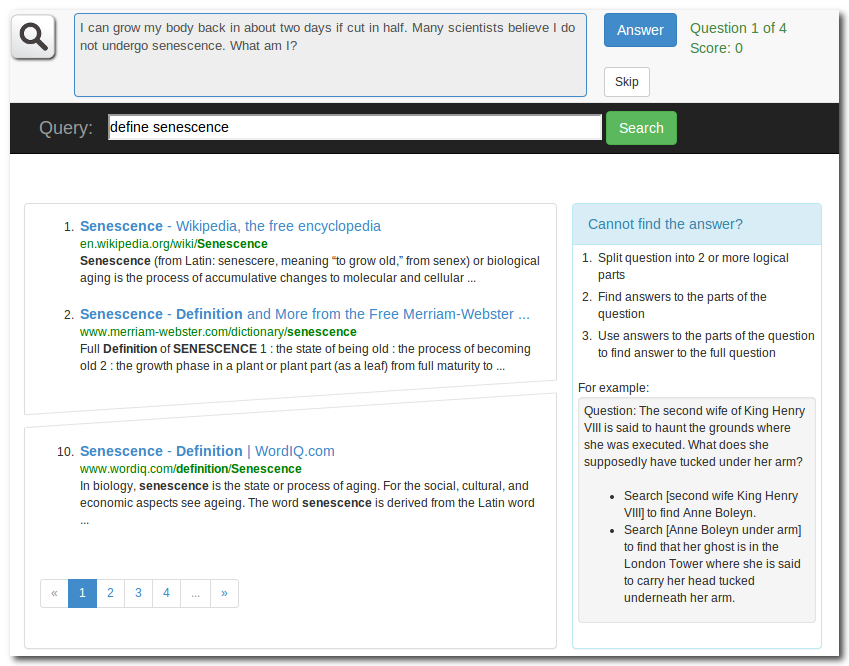
\includegraphics[width=0.75\textwidth]{img/hints_ufindit}
\caption{The interface of the search game used in the study of the effect of strategic search hints on success in solving complex informational tasks}
\label{figure:users:hints:ufindit}
\end{figure}

To estimate the effect of strategic search hints on user behavior we conducted a study in a form of a web search game similar to ``a Google a Day''\footnote{http://www.agoogleaday.com/} and uFindIt \cite{Ageev:2011:FYG:2009916.2009965}. Participants were hired using Amazon Mechanical Turk\footnote{http://www.mturk.com/}. 

The goal of the web search game used in the user study is to find answers to several questions with the provided web search interface (Figure \ref{figure:users:hints:ufindit}). 
Players are instructed not to use any external tools.
The questions are given one by one and since tasks might be too difficult, a chance to skip a question was provided, although users were instructed that effort put into solving a question will be evaluated.
To answer a question each player needs to provide a link to a page containing the answer as well as its text.
The answer is automatically verified and a popup box notifies a player if the answer is incorrect (since the answer can be formulated differently, presence of a keyword was checked).
A player can then continue searching or skip the question when she gives up.
A bonus payment was made to players who answer all questions correctly.
We used Bing Search API\footnote{http://www.bing.com/toolbox/bingsearchapi} as a back-end of the game search interface.
All search results and clicked documents were cached so users asking the same query or clicking the same page got the same results.
At the end of the game a questionnaire was presented asking for feedback on user satisfaction with the game, prior experience and other comments.

\begin{table}[tbh]
\centering
\begin{tabular}{|p{1cm}|p{4.5cm}|p{4.2cm}|p{6.0cm}|} \hline
 & Question & Correct Answer & Specific hints \\ \hline
Task 1 & I can grow body back in about two days if cut in half. Many scientists think I don't undergo senescence. What am I? & Senescence means ``biological aging''. Hydra is considered biologically immortal and regenerates fast. & \parbox[t]{6cm}{
1. Find what is senescence \\
2. Find who does not undergo senescence \\
3. Find who can also regenerate body and choose the one that satisfies both conditions} \\\hline
Task 2 & Of the Romans "group of three" gods in the Archaic Triad, which one did not have a Greek counterpart? & Archaic Triad includes Jupiter, Mars and Quirinus. Among those Quirinus didn't have a Greek counterpart. &
\parbox[t]{6cm}{
1. Find the names of the gods from the Archaic triad\\
2. For each of the gods find a Greek counterpart
}\\ \hline
Task 3 & As George surveyed the ``waterless place'', he unearthed some very important eggs of what animal? & "Gobi" in Mongolian means ``Waterless place''. The first whole dinosaur eggs were discovered there in 1923. & \parbox[t]{6cm}{
1. Find what is the ``waterless place'' mentioned in the question?\\
2. Search for important eggs discovery in this ``waterless place''}\\ \hline
Task 4 & If you were in the basin of the Somme River at summers end in 1918, what language would you have had to speak to understand coded British communications? & Cherokee served as code talkers in the Second Battle of the Somme. & \parbox[t]{6cm}{
1. Find the name of the battle mentioned in the questions\\
2. Search for which coded communications language was used in this battle\\
} \\ \hline
\end{tabular}
\caption{Search tasks used for the study, and specific search hints shown to one of the user groups}
\label{table:users:hints:tasks}
\end{table}

The tasks for the study were borrowed from the ``A Google a Day'' questions archive.
Such questions are factual, not ambiguous and usually hard to find the answer with a single query, which makes them interesting for user assistance research.
We filtered search results to exclude all pages that discuss solutions to ``A Google a Day'' puzzles.
To do this we removed pages that mention a major part of the search question or ``a google a day'' phrase.
To keep users focused throughout the whole game we limited the number of questions to 4.
The tasks are described in Table \ref{table:users:hints:tasks} and were presented to all participants in the same order to ensure comparable learning effects.

The questions have multiple parts and to solve them it is helpful to search for answers to parts of the questions and then combine them.
In one of the previous studies we observed, that most of the users didn't adopt the divide-and-conquer strategy, but kept trying to find the ``right'' query.
We decided to estimate the effect of strategic search hints, suggesting users to adopt the new strategy.

We built 2 sets of strategic hints: \textit{task specific} and \textit{generic}.
Task-specific hints described steps of one of the possible solutions to each question (Table \ref{table:users:hints:tasks}).
Second set contained a single hint, which was shown for all tasks. Generic hint described the divide-and-conquer strategy:\\
\hrule
\begin{enumerate}
\item Split the question into 2 or more logical parts
\item Find answers to the parts of the question
\item Use answers to the parts of the question to find answer to the full question
\end{enumerate}

For example, the question: ``The second wife of King Henry VIII is said to haunt the grounds where she was executed. What does she supposedly have tucked under her arm?''
\begin{enumerate}
\item Search [second wife King Henry VIII] to find Anne Boleyn.
\item Search [Anne Boleyn under arm] to find that her ghost is in the London Tower where she is said to carry her head tucked underneath her arm.
\end{enumerate}
\hrule

To control for the learning effect demonstrated in \cite{Moraveji:2011:MIU:2009916.2009966}, each user was assigned to one of the three groups:
\begin{enumerate}
\item users who didn't get any hints
\item users who got task-specific hints
\item users who got the generic hints
\end{enumerate}


\subsubsection{Results}
\label{section:users:hints:results}

From 199 unique participants, who clicked the HIT on Amazon Mechanical Turk only 90 players finished the game.
We further examined all games manually and filtered out 9 submissions for one of the following reasons: lack of effort (e.g. skipped several tasks after none or a single query) or usage of external resources (e.g. the answer was obtained without submitting any queries or results explored didn't contain the answer).
Furthermore, 10 players from the group which received hints indicated in the survey that they didn't see them, so we filtered out those submissions and finally we had 71 completed games (29 for no hints, 20 for task-specific hints and 22 for generic hints groups).

\textbf{Effects of Search Tips on Performance}.
In order to measure search success rate we looked at the number of questions answered correctly by different groups of users\footnote{Since users were allowed to skip a question we are counting the number of questions that were eventually solved correctly even if a player made some incorrect attempts}.
Figure \ref{figure:users:hints:task_success} shows that success rate is higher for users who saw task-specific hints compared to users who didn't get such assistance.
Surprisingly, having the generic hint decreased the success rate, although users could easily ignore a hint they didn't like.
A possible explanation is: generic hints were harder to follow and users who tried and failed became frustrated and didn't restart their searches.

The plot of average time to answer a question on Figure \ref{figure:users:hints:task_time} doesn't show an improvement for the task-specific hints group, except for the question 1.
Our task-specific hints represent a possible way to solve a problem and there is no guarantee, that it is the fastest one.
It is worth noting, that users from the generic search hint group had slightly higher variance in success time, which can probably be explained by the fact that some users were successful in finding the right way to follow the hint and some other users struggled with it much longer.
Another insight comes from the number of incorrect attempts users made.
Figure \ref{figure:users:hints:incorrect} demonstrates the average number of incorrect answer attempts for all groups of users.
Although the variance is high, there is a tendency for users who saw task-specific hints to make less attempts than both other groups.
This is not in direct correspondence with time spent on the game.
It seems that the users who saw a clear strategy to solve the question were less likely to notice plausible, but incorrect solution.
Moreover, we analyzed texts of incorrect answers, and can conclude that a big part of incorrect submission are due to users trying all possible options they found on the way, even if these options are clearly wrong.


\begin{figure}[h]
\centering
  \begin{subfigure}{0.32\textwidth}
  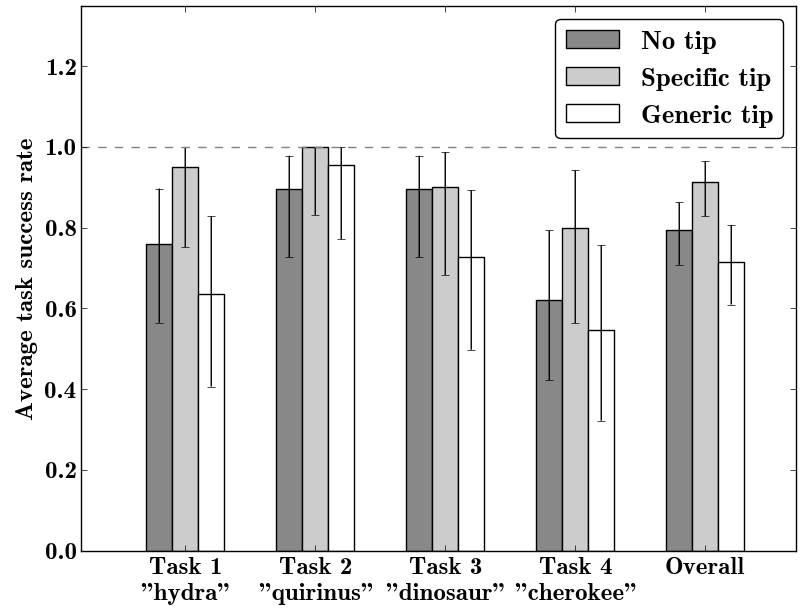
\includegraphics[width=\textwidth]{img/hints_success_per_task}
  \caption{Success rate per task for each group of participants}
  \label{figure:users:hints:task_success}
  \end{subfigure}
  \begin{subfigure}{0.32\textwidth}
  \centering
  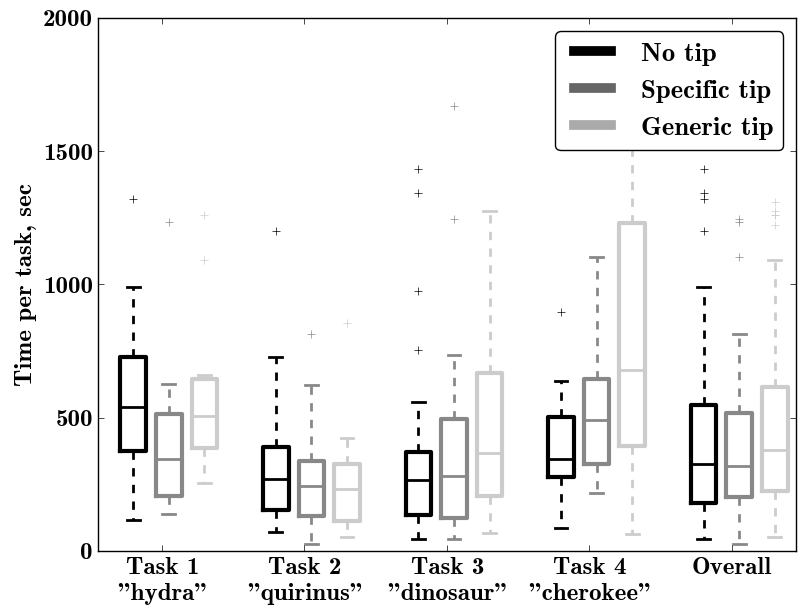
\includegraphics[width=\textwidth]{img/hints_time_per_task}
  \caption{Task completion time for each group of players}
  \label{figure:users:hints:task_time}
  \end{subfigure}
  \begin{subfigure}{0.32\textwidth}
  \centering
  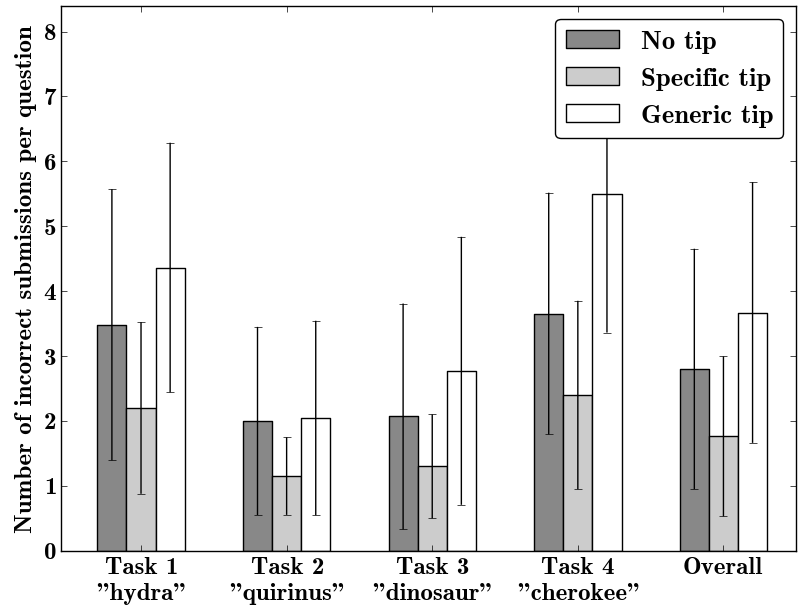
\includegraphics[width=\textwidth]{img/hints_incorrect}
  \caption{The number of incorrect submission attempts per question for all groups of users}
  \label{figure:users:hints:incorrect}
  \end{subfigure}
\caption{Results of the user study on the effectiveness of strategic search tips on search task success rate}
\label{fig:users:hints:results}
\end{figure}

\begin{figure}[h]
\centering
\begin{subfigure}[t]{0.32\textwidth}
	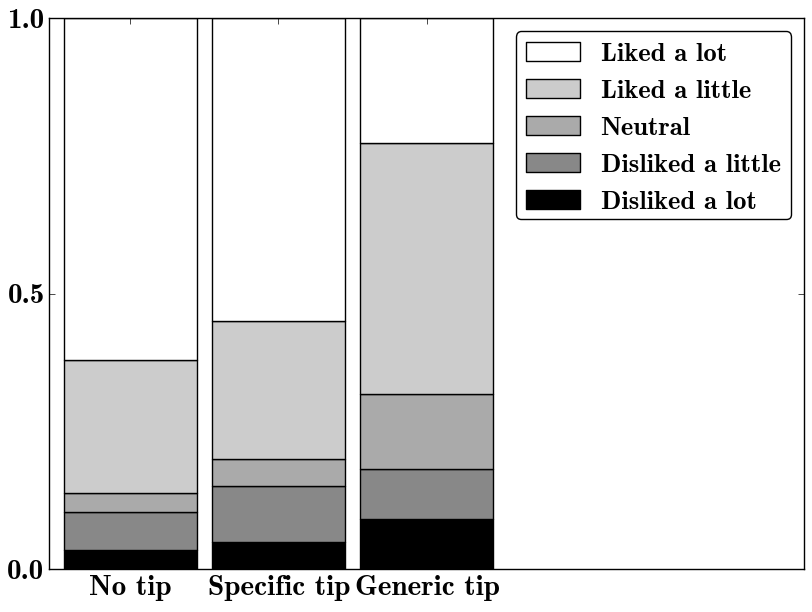
\includegraphics[scale=0.26]{img/hints_liked}
	\caption{How did you like the game?}
    \label{figure:users:hints:survey:liked}
\end{subfigure}
\begin{subfigure}[t]{0.32\textwidth}
	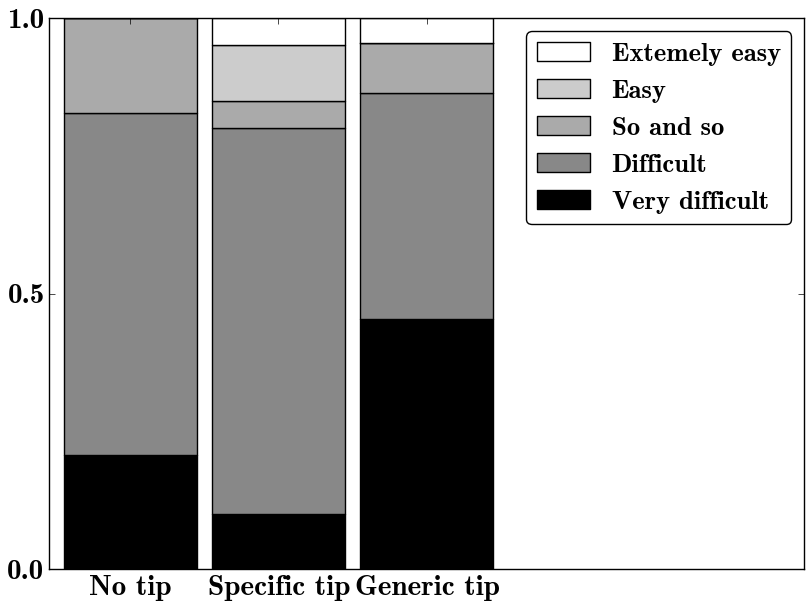
\includegraphics[scale=0.26]{img/hints_difficult}
	\caption{How difficult was the game?}
    \label{figure:users:hints:survey:difficult}
\end{subfigure}
\begin{subfigure}[t]{0.32\textwidth}
	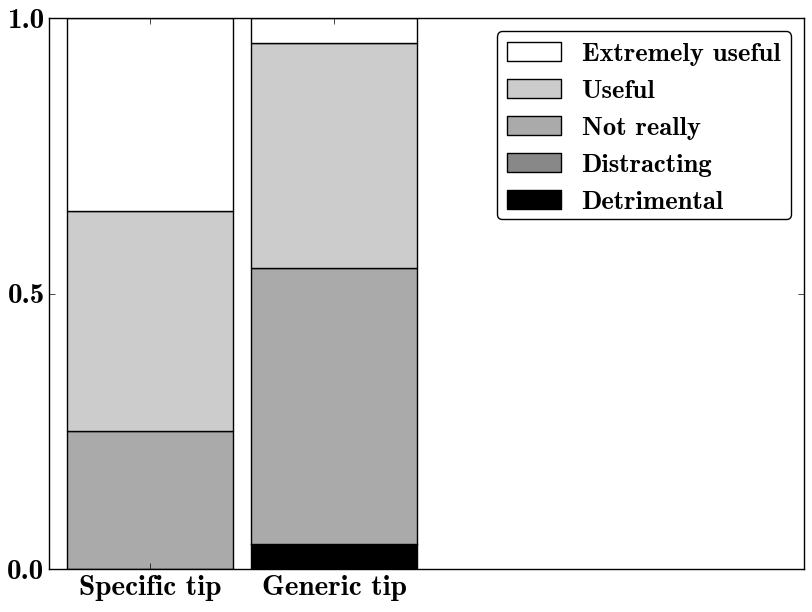
\includegraphics[scale=0.26]{img/hints_useful}
	\caption{Were search hints useful to you?}
    \label{figure:users:hints:survey:useful}
\end{subfigure}
\caption{Proportions of replies to some of the survey question for each group of users}
\label{figure:users:hints:survey}
\end{figure}

We also looked at other search behavior characteristics: number of queries submitted, number of clicks made, average length of the queries. The variance in these characteristics was too high to make any speculations regarding their meaning.

\textbf{Effects of Search Tips on User Experience}.
Finally, we looked at the surveys filled out by each group of users.
Figure \ref{figure:users:hints:survey} presents proportions of different answers to three of the questions: ``How did you like the game?'', ``How difficult was the game?'' and ``Were search hints useful to you?''.
Surprisingly, user satisfaction with the game was lower for users who saw hints during the game and users who didn't get any assistance enjoyed it more.
The replies to the question about game difficulty are in agreement with the success rate: users who saw task-specific hints rated difficulty lower than participants who struggled to find the correct answers.
The game was very difficult on average, however, some participants from the group who received task-specific hints surprisingly rated it as very easy, which suggests that our hints do help users.
This is supported by the answers to the last question on whether hints were helpful (Figure \ref{figure:users:hints:survey:useful}).

To summarize, the results of the conducted user study suggest that specific search hints can be helpful, which is indicated by higher success rate, lower number of incorrect attempts and positive feedback in the end of study survey.
In contrast, generic hints can have negative effect on user experience, which is indicated by lower success rate, increased number of incorrect attempts and higher perceived tasks complexity according to the survey.

\subsubsection{Summary}
\label{section:users:hints:summary}

In this section we studied the effect of strategic search hints on user behavior. 
The conducted user study in a form of a web search game demonstrated the potential of good hints in improving search success rate.
However, to be useful, they should be designed carefully.
Search hints that are too general can be detrimental to search success.
We also find that even searchers who are more effective using specific search hints, feel subjectively less satisfied and engaged than the control group, indicating that search assistance has to be specific and timely if it is to improve the searcher experience.

Even though strategic search hints can improve success rate for complex informational tasks, they represent a rather one-way form of communication, where a system doesn't accept any feedback from the user and doesn't adapt to it.
Hints essentially outsource all the heavy-lifting of decision making to the user, which often makes the experience less enjoyable, as demonstrated by the post-study survey results.
An alternative strategy is to let the system adapt based on the implicit and explicit feedback from the user.
Such a scenario looks even more compelling given a proliferation of personal assistants and chat bots, which makes it easy for users to respond to the user answer with either positive or negative feedback message.

%-=-=-=-=-=-=-Search hints end-=-=-=-=-=-

\section{Proposed Research}
\label{section:users:proposal}

Question answering is one of the major components of modern personal assistants like Apple Siri, Amazon Alexa and Microsoft Cortana.
However, these systems still operate in one sided communication mode, where a user formulates queries and assistant responds with an answer or search results.
In my thesis I propose to incorporate feedback from the user to improve the performance of the question answering system.
To make it more concrete, consider an Example on Figure~\ref{figure:users:proposal:example}.
It's not uncommon for a question answering system to be incorrect.
Web search engines typically decide whether to show direct answers or not based on the confidence in the answer~\cite{yang2015wikiqa}.
However, in a dialog a system needs to provide some kind of response, and why not take a chance and return the top candidate answer.
If the user doesn't like the answer, she can respond accordingly, and this feedback needs to be taken into account by the question answering system, which can then re-rank the candidate answers and provide an alternative response, that will hopefully satisfy the user.

\begin{figure}
\centering
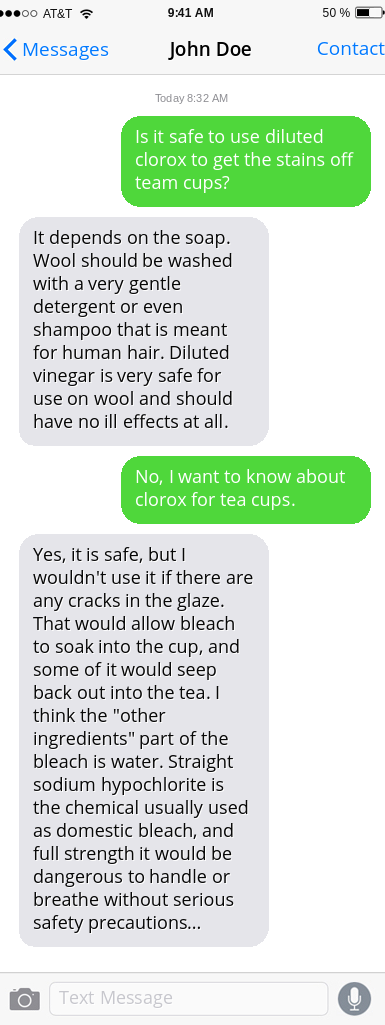
\includegraphics[width=0.3\textwidth]{img/chatbot_example}
\caption{An example of a dialog-based question answering system, that accepts feedback from the user and returns an updated answer}
\label{figure:users:proposal:example}
\end{figure}

Relevance feedback has been studied extensively in the information retrieval community for ad-hoc document retrieval~\cite{salton1997improving,rocchio1971relevance,wang2008study}, but not for question answering.
Thus, I propose to explore the methods for relevance feedback in question answering.

\subsection{Method}
\label{section:users:proposal:method}

In my thesis I propose to focus on both positive and negative relevance feedback for question answering.
A user might give a system a positive feedback if the provided answer was relevant, but either alternative view or additional information is needed.
Alternatively, if an answer is not helpful, a system can take negative feedback to try to generate a good answer.

As a baseline for the experiments I'm planning to take the system I developed for TREC LiveQA shared task, described in Section~\ref{section:non-factoid:liveqa:architecture}, and extend it with the relevance feedback module.
This module will allows the system to adjust and return an alternative answer given either positive or negative feedback.
I'm going to integrate relevance feedback into the system's candidate ranking model.
More specifically, a set of features representing a candidate answer will be extended with various scores, that measure syntactic and semantic similarities between a candidate and positive and negative feedback examples.
This additional set of features will include various vector space, distributed semantics~\cite{kusner2015word} and language model similarity scores~\cite{wang2008study}, as well as some more simple statistics, such as common and missing n-grams, longest common substrings, \etc.
The overall architecture of the proposed system is sketched on Figure~\ref{figure:users:proposal:model}.

There are other alternative stages in the QA pipeline, where we could incorporate the relevance feedback, \eg a system can adjust a set of search queries used to retrieve a set of candidates as done for ad-hoc information retrieval~\cite{rocchio1971relevance}, but I will have to leave this for future work.

\begin{figure}
\centering
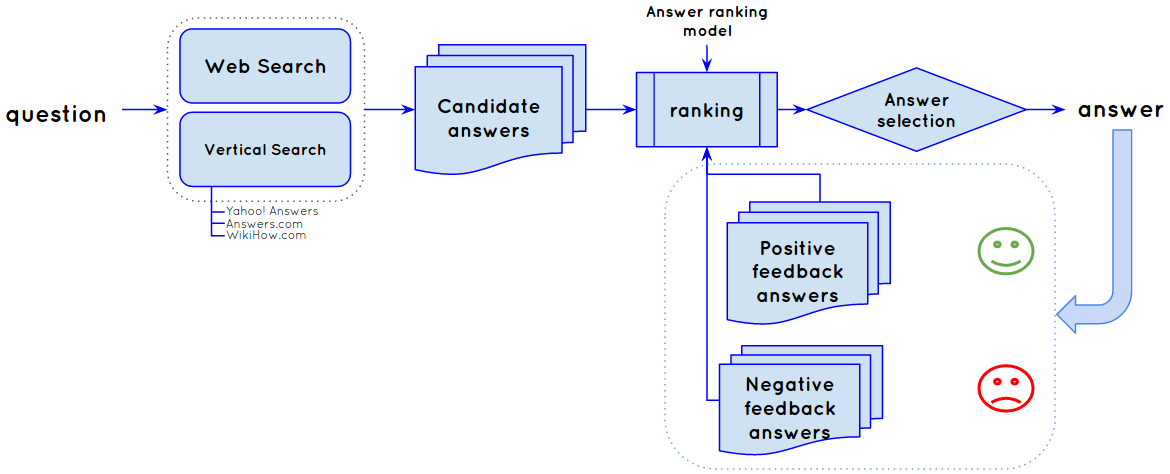
\includegraphics[width=\textwidth]{img/userfeedback_model}
\caption{Architecture of the question answering system, that incorporate positive and negative relevance feedback}
\label{figure:users:proposal:model}
\end{figure}

\subsection{Experimentation}
\label{section:users:proposal:experiments}

To test the system experimentally I propose to reuse the data from TREC LiveQA 2016, which we collected for the crowdsourcing experiment (see Section~\ref{section:crowdsourcing:approach:crqa:experiments}).
As a remainder, during the official run of TREC LiveQA 2016 we collected 1087 questions, issued to our system.
For each question, top 7 generated candidate answers were rated by crowd workers on a scale from 1 (bad) to 4 (excellent).

To test the proposed relevance feedback model I'm proposing to conduct the following simulation experiment.
For each question, top 7 answers will be arranged according to their model score.
Assuming the model returns the top candidate, we collect cases when the top candidate has a low relevance score (\eg $score < 2$), and use these answers as negative feedback.
The goal of the model will be to re-rank the rest of the candidates and return a better answer.
A baseline in this experiment will be a system, that doesn't use the feedback and simply returns the next best answer according to the model score.
Positive relevance feedback experiment will be conducted in a similar way: all answers with good relevance score (\eg from 2 to 3) will be given back to the system as positive feedback with the goal to return another good answer.
This experiment will help us confirm or reject the hypothesis, that it's possible to incorporate relevance feedback for question answering.

To train our ranking model to accept additional answer candidates I will split the original dataset into training and test parts again.
Using the original model I will collect cases with negative and positive feedback as described above, and train the model to retrieve the best possible candidate from the rest of the answers.

However, such simulation experiment won't allow us to test if relevance feedback improves the user experience.
To answer this question we will conduct a user study using either Mechanical Turk or hire some student workers.
We are building a chatbot for Facebook messenger, that will serve as a front-end to our question answering system.
The users will receive a set of questions, e.g. sampled from Yahoo! Answers, and will need to get a satisfactory answer using our chatbot.
All the users will be split into two groups: with and without an option to leave relevance feedback.
The relevance feedback group will be asked to mark each answer as good or bad, after which a new candidate will be provided until the user will decide to stop and declare either fail or success.
The group without relevance feedback will be given an option to receive another answer, which will simply be the next candidate in the original ranked list.
Upon completion of all tasks, the users will complete the questionnaire, where I will ask questions about their experience and satisfaction with the chatbot.
Task success rate and the feedback will help me answer the question if relevance feedback for question answering improves user experience.

\section{Summary}
\label{section:users:summary}

In this chapter I described my prior and proposed research in improving user experience with question answering systems.
Strategic hints, that a system might display to help the user better split the original problem, were shown to be able to improve the success rate, however they need to be designed carefully.
Hints, that are too generic and hard to follow can be distracting and detrimental to the user experience.
However, such hints put all the hard work on the user, who will go through the trial and error process until a system is able to retrieve a good answer.
The second part of the section described the proposed research in engaging in a dialog with the user, and using these interactions to receive relevance feedback, which can be used to refine the answer.
I believe that this feedback is one of the first step, that can lead to deeper understanding of user information needs through dialog.


% chap7_proposal.tex
%

\mychapter{Summary \& Research Proposal}
\label{chapter:proposal}

\noindent

This chapter summarized the research I propose to do in my thesis to improve different aspects of question answering.

\section{Research Objectives}
\label{section:proposal:objectives}

The main research objectives I plan to target in my thesis are the following:

\begin{enumerate}
\item RQ1. How to effectively combine unstructured text and structured knowledge base data to improve factoid question answering?
\item RQ2. How to improve candidate retrieval and answer generation for non-factoid question answering?
\item RQ4. How to use crowdsourcing to improve question answering performance in near real-time scenario?
\item RQ3. How to utilize the dialog between the user and question answering system to improve users success rate in solving informational tasks?
\end{enumerate}

\section{Research Plan}
\label{section:proposal:plan}

\subsection{Combining KB and Text Data for Factoid Question Answering (Chapter \ref{chapter:factoid})}
\label{section:proposal:plan:factoid}

Structured and unstructured data sources, such as knowledge bases and text document collections, are quite effective for factoid question answering.
However, these data sources are quite different in nature and in many cases can compliment each other.
Two major issues with KBQA is knowledge base incompleteness and complexity of translating natural language question into a structured query.
Text documents on the other hand are easier to match against the question, contain more information than a typical knowledge base, but aggregating information across multiple statements and documents is complicated.

One way to improve the situation with knowledge base incompleteness is to extract missing information from other data sources, \eg \cite{Cafarella:2008:WEP:1453856.1453916,Cafarella:2009:WES:1519103.1519112,Dong:2014:KVW:2623330.2623623,Etzioni:2008:OIE:1409360.1409378,Gupta:2014:BOS:2732286.2732288,kushmerick1997wrapper}.
In my prior research I proposed to get use of one additional data source, that wasn't used for relation extraction before, namely question-answer pairs.
Section~\ref{section:factoid:approaches:cqarelextract} described the experiments and results in utilizing this data to improve knowledge base coverage.

Unfortunately, relation extraction isn't perfect either and there are both precision and recall losses.
Therefore, in my thesis I propose to explore semantic annotation of entity mentions as a way to bridge the gap between KB entity graph and text documents.
Such representation will allow us to do simple string matching on text documents and at the same time explore the knowledge about the mentioned entities in KB and vice versa.
The idea of the proposed approach is based on extending a set of links in a knowledge base with edges connecting entities to their mentions in text documents.
Therefore, text fragments, that mention two or more entities, essentially create additional edges in the knowledge base connecting these entities, and these edges are ``labelled'' with textual representation of the fragment (e.g. bag of words or embedding).
Section~\ref{section:factoid:proposal} described the proposed approach in more detail.

\subsubsection{Expected contributions}
\label{section:proposal:plan:factoid:contributions}

\begin{itemize}
\item A novel model for relation extraction from archives of question-answer pairs.

The developed model allows to extract relational triples for KB completion from a novel data source.
The experiments demonstrate, that together with existing sentence-based relation extraction techniques it is now possible to get more information, which eventually benefits the performance of knowledge base question answering and other downstream KB applications.

\item New hybrid KB-Text question answering approach, that improves knowledge base question answering by using information from unstructured text data sources, annotated with KB entity mentions, which essentially introduces a new types of edges into a knowledge graph
% that operates by searching an entity graph, built from both facts from a KB and links between KB entities and text fragments mentioning these entities

The proposed model has a potential to overcome many of the issues of KB and text question answering, and allow to answer complex factual questions, that couldn't be answered before.
This research could be useful for future work on integrating different unstructured, semi-structured and structured data sources for joint reasoning in question answering and other applications.

\end{itemize}

\subsubsection{Risks}
\label{section:proposal:plan:factoid:risks}

\begin{itemize}
\item The dataset I propose to derive from CQA data might be hard to build due to potentially low number of questions, that survive the filtering. In case this happens I will have to use one of the other existing datasets, such as TREC QA.
\item Abundant textual information might add a lot of noise to our knowledge graph extended with text-based edges. More connections means more candidates for our search algorithm, and increased level of noise might be hard to deal with in this scenario, which could actually drop the performance compared to clean, but incomplete knowledge base only model.
\end{itemize}


\subsection{Answer Summarization for Non-factoid Question Answering (Chapter~\ref{chapter:non-factoid})}
\label{section:proposal:plan:non-factoid}

A typical approach for non-factoid question answering is to retrieve passages from either answers to existing questions in CQA archives or from regular web documents.
Quite often such passages contain some redundant information, that the user didn't ask for in her question, or on the contrary a single passage cannot completely satisfy user information needs.
In Section~\ref{section:non-factoid:proposal} I proposed to develop answer summarization techniques, inspired by the recent advances in deep learning for text summarization \cite{rush-chopra-weston:2015:EMNLP,chopraabstractive16} and generation \cite{karpathy2015deep}.
More particularly, I'm planning to test both extractive and abstractive text summarization approaches on the task of generating responses to non-factoid questions.

\subsubsection{Expected contributions}
\label{section:proposal:plan:non-factoid:contributions}

\begin{itemize}
\item An open source non-factoid question answering system, designed to participate in TREC LiveQA shared task, and which can be used as a baseline in various experiments in improving different aspects of the QA process.

The system I developed was ranked top-7 in TREC LiveQA 2015 shared task (the results of the 2016 track aren't yet available).

\item A novel answer summarization module for non-factoid question answering system.
Unlike some prior work, which focused on summarizing answers posted by different users on CQA platforms, the model I propose to develop will operate inside a real question answering system, which means it will have to deal with some additional challenges, such as higher rate of irrelevant passages.
This model will be useful as a first step towards more sophisticated answer distillation techniques~\cite{mitra2016distillation}.

\end{itemize}

\subsubsection{Risks}
\label{section:proposal:plan:non-factoid:risks}

\begin{itemize}
\item The amount of training data available for the task isn't that big compared to some other datasets, used to train deep learning models. There is a risk, that it won't be enough to find the optimal parameters for the model and beat some traditional techniques
\end{itemize}

\subsection{Crowdsourcing for near Real-time Question Answering (Chapter~\ref{chapter:crowdsourcing})}
\label{section:proposal:plan:crowdsourcing}

In Section~\ref{section:crowdsourcing:approach} I described the approach we took to integrate question answering into a real-time non-factoid question answering system.
The results of our studies demonstrated that crowd workers can easily rate the quality of candidates and even provide their own answers to questions in under 1 minute time limit.
We integrated the crowdsourcing module into our TREC LiveQA system to participate in the 2016 run of the shared task.
To make the hybrid system real-time we used the retention model~\cite{bernstein2011crowds} to have a set of workers waiting for a new question to arrive.
When our QA system receives a question, it posts it to the workers, who can now read the question and decide if they can provide the answer themselves.
In the meantime, the automatic system works to retrieve a set of candidate answers from various resources and rank them.
Next, top 7 candidates are send for labeling to workers, who can now judge the relevance of each of the presented answers.
The system waits for the response until the maximum response time of one minute for a question is near, retrieves all the crowdsourcing feedback and performs the final answer reranking.
The results of our preliminary analysis of data we gathered during TREC LiveQA 2016 revealed that with worker feedback, the system was able to significantly improve its performance.

The focus of the follow up research I proposed to do for my thesis is on optimizing the costs of the proposed approach.
To make our system more scalable and cut the costs associated with the crowdsourcing module, I propose to incorporate a model to predict the expected performance of the answer, generated by the automated system.
This score can be used to prioritize tasks when the load is high, and even skip some tasks altogether, if the expected quality of automatically generated answer is high.

\subsubsection{Expected contributions}
\label{section:proposal:plan:crowdsourcing:contributions}

\begin{itemize}
\item New method for answer collection and rating using crowdsourcing for a near real-time question answering system.

I believe that this piece of work could be very useful for future research on the interaction between automated QA and dialog systems and human experts, which could be essential to modern intelligent assistants.
Existing systems works great for a subset of user tasks, but encounter certain problems for a different subset.
To provide a smooth user experience it might be crucial to have a fall back option of human experts, who can help systems to overcome the challenge.

\item A novel hybrid question answering system, that incorporates crowdsourcing, but still operates in near real-time, \ie providing a response within one minute after the question is posted.
This is much faster than on existing community question answering platforms, where a quarter of the questions are left completely unanswered.
\end{itemize}

\subsubsection{Risks}
\label{section:proposal:plan:crowdsourcing:risks}

\begin{itemize}
\item High overall costs of the developed crowdsourcing module.
In the current version of our hybrid question answering system, developed for TREC LiveQA 2016 the cost of a single question turned out to be \$0.81, which is quite a lot.
The proposed research targets the problem of reducing these costs by applying crowdsourcing selectively, but there is a risk that the cost of getting a significant quality improvement will still be high to make our system practically useful.
\end{itemize}

\subsection{User Interactions with Question Answering Systems (Chapter~\ref{chapter:users})}
\label{section:proposal:plan:users}

In my thesis I'm going to focus to a tiny part of all possibilities, that are opened up by a full power dialog between a user and a question answering system.
In my prior research I considered search hints, as a means to give user some suggestions on how to proceed with complex informational tasks.
Well-designed hints turned out to be quite helpful, and improved user success rate.
However, one needs to be careful with such a tool, as hints that are too general and hard to implement can be detrimental to user experience.

To take some hard work off the user, I'm also proposing to develop methods for positive and negative relevance feedback in a question answering dialog scenario.
After a system returns an answer, a user might respond with certain feedback, whether positive (\eg ``give me more information on the topic'') or negative (\eg ``this answer is bad'').
The system needs to take this feedback into account and come up with a better answer.
To implement this functionality I propose to extend a set of features representing each answer candidates with features, measuring similarities and dissimilarities between the candidate and provided positive and negative feedback answers.
More details on the architecture of the proposed approach are given in Section~\ref{section:users:proposal:method}.

\subsubsection{Expected contributions}
\label{section:proposal:plan:users:contributions}

\begin{itemize}
\item A study of the effect of strategic search hints on the user experience and success rate for complex informational tasks.

The results of this work suggest, that well designed search hints can have a positive effect on users struggling with a complex search task.
These observations provide some insights for future research in user assistance for complex information needs.

\item A novel method for positive and negative relevance feedback in a question answering dialog scenario. 
I believe that incorporating user feedback is a first step towards a richer dialog between a computer system and a user.
In future, it's possible to extend a set of dialog actions and allow system ask clarification questions or confirm certain pieces of information.
\end{itemize}

\subsubsection{Risks}
\label{section:proposal:plan:users:risks}

\begin{itemize}
\item Negative relevance feedback is usually harder to implement that positive feedback~\cite{wang2008study}.
Negative feedback tells the system some information on what user didn't like.
However, the space of irrelevant information is much larger than relevant, \ie another candidate answer might be different from the one that received negative feedback, but still doesn't provide any useful information.
Therefore, if in our scenario bad questions turns out to be quite diverse, negative feedback might not work efficiently, and the overall user experience would suffer.
\end{itemize}

\section{Research Timeline}
\label{section:proposal:timeline}

A tentative timeline for the work that needs to be done is shown below:

\begin{itemize}
\item Joint model for question answering over KB and text (Section~\ref{section:factoid:problem}): \textit{8/2016}
	\begin{enumerate}
	\item collect and index textual data about entity mentions from ClueWeb12 dataset
	\item derive a factoid question answering dataset from Yahoo!Answers WebScope collection
	\item build a joint KB and text question answering system
	\item test it on existing (TREC QA) as well is derived datasets and compare the results with the baselines
	\end{enumerate}
	
\item Optimizing crowdsourcing for near real-time question answering (Section~\ref{section:crowdsourcing:proposal}): \textit{9/2016}
	\begin{enumerate}
	\item build a model to predict the expected quality of automatically generated answer candidate
	\item develop a task scheduling system based on priorities estimated in step 1, number of workers available and the current load of the system.
	\item test the system by simulating arrivals of the question using different models
	\end{enumerate}

\item Answer summarization for non-factoid question answering (Section~\ref{section:non-factoid:proposal}): \textit{10/2016}
	\begin{enumerate}
	\item build a model for extractive summarization for non-factoid question answering
	\item if time permits, build a model for abstractive summarization for non-factoid question answering
	\item test the model on Yahoo! Answers datasets from~\cite{omari2016novelty,tomasoni2010metadata}
	\item integrate the model into my TREC LiveQA system, test it on a set of questions and manually judge the quality compared to a single returned answer.
	\end{enumerate}

\item Relevance feedback for dialog-based question answering (Section~\ref{section:users:proposal}): \textit{11/2016}
	\begin{itemize}
	\item implement features to measure similarity between an answer candidate and negative and positive feedback answers
	\item train candidate answer ranking model, that incorporates relevance feedback if available
	\item test the model on the data from TREC LiveQA 2016
	\item conduct a small user study to see how the system behaves in a real scenario and whether or not it improves the user experience
	\end{itemize}

\item Thesis writing: \textit{10/2016 - 11/2016}
\item Thesis defense: \textit{12/2016}
\end{itemize}

\section{Summary}
\label{section:proposal:summary}

In my thesis I proposed several pieces of work towards improving user satisfaction with question answering systems for factoid as well as non-factoid information needs.
The proposed research spans multiple directions: from improving the data sources for factoid question answering, better answer representation by summarizing available pieces of information, to engaging the human input, either from a crowd of external workers or the user herself in a form of feedback.
I believe, that the results of the proposed research directions will be useful for the developing field of intelligent personal assistants and chat bots, as question answering is arguably one of their most important applications.


% \appendix
% \include{appendixa}
% \include{appendixb}
% \include{appendixc}
%%%%%%%%%%%%%%%%%%%%%%%% STOP EDITING HERE %%%%%%%%%%%%%%%%%%%%%%%%

\bibliographystyle{abbrv}\small 
\setlength{\bibsep}{2pt}
\singlespacing
\bibliography{References}

\end{document}
